%%%%%%%%%%%%%%%%%%%%%%%%%%%%%%%%%%%%%%%%%%%%%%%%%%%%%%%%%%%%%%%%%%%%%%
% Template for a UBC-compliant dissertation
% At the minimum, you will need to change the information found
% after the "Document meta-data"
%
%!TEX TS-program = pdflatex
%!TEX encoding = UTF-8 Unicode

%% The ubcdiss class provides several options:
%%   gpscopy (aka fogscopy)
%%       set parameters to exactly how GPS specifies
%%         * single-sided
%%         * page-numbering starts from title page
%%         * the lists of figures and tables have each entry prefixed
%%           with 'Figure' or 'Table'
%%       This can be tested by `\ifgpscopy ... \else ... \fi'
%%   10pt, 11pt, 12pt
%%       set default font size
%%   oneside, twoside
%%       whether to format for single-sided or double-sided printing
%%   balanced
%%       when double-sided, ensure page content is centred
%%       rather than slightly offset (the default)
%%   singlespacing, onehalfspacing, doublespacing
%%       set default inter-line text spacing; the ubcdiss class
%%       provides \textspacing to revert to this configured spacing
%%   draft
%%       disable more intensive processing, such as including
%%       graphics, etc.
%%

% For submission to GPS
\documentclass[gpscopy,onehalfspacing,11pt]{ubcdiss}
\usepackage{rotating}
% For your own copies (looks nicer)
% \documentclass[balanced,twoside,11pt]{ubcdiss}

%%%%%%%%%%%%%%%%%%%%%%%%%%%%%%%%%%%%%%%%%%%%%%%%%%%%%%%%%%%%%%%%%%%%%%
%%%%%%%%%%%%%%%%%%%%%%%%%%%%%%%%%%%%%%%%%%%%%%%%%%%%%%%%%%%%%%%%%%%%%%
%%
%% FONTS:
%% 
%% The defaults below configures Times Roman for the serif font,
%% Helvetica for the sans serif font, and Courier for the
%% typewriter-style font.  Configuring fonts can be time
%% consuming; we recommend skipping to END FONTS!
%% 
%% If you're feeling brave, have lots of time, and wish to use one
%% your platform's native fonts, see the commented out bits below for
%% XeTeX/XeLaTeX.  This is not for the faint at heart. 
%% (And shouldn't you be writing? :-)
%%

%% NFSS font specification (New Font Selection Scheme)
\usepackage{times,mathptmx,courier}
\usepackage[scaled=.92]{helvet}

%% Math or theory people may want to include the handy AMS macros
\usepackage{amssymb}
\usepackage{amsmath}
\usepackage{amsfonts}

%% The pifont package provides access to the elements in the dingbat font.   
%% Use \ding{##} for a particular dingbat (see p7 of psnfss2e.pdf)
%%   Useful:
%%     51,52 different forms of a checkmark
%%     54,55,56 different forms of a cross (saltyre)
%%     172-181 are 1-10 in open circle (serif)
%%     182-191 are 1-10 black circle (serif)
%%     192-201 are 1-10 in open circle (sans serif)
%%     202-211 are 1-10 in black circle (sans serif)
%% \begin{dinglist}{##}\item... or dingautolist (which auto-increments)
%% to create a bullet list with the provided character.
\usepackage{pifont}

%%%%%%%%%%%%%%%%%%%%%%%%%%%%%%%%%%%%%%%%%%%%%%%%%%%%%%%%%%%%%%%%%%%%%%
%% Configure fonts for XeTeX / XeLaTeX using the fontspec package.
%% Be sure to check out the fontspec documentation.
%\usepackage{fontspec,xltxtra,xunicode}	% required
%\defaultfontfeatures{Mapping=tex-text}	% recommended
%% Minion Pro and Myriad Pro are shipped with some versions of
%% Adobe Reader.  Adobe representatives have commented that these
%% fonts can be used outside of Adobe Reader.
%\setromanfont[Numbers=OldStyle]{Minion Pro}
%\setsansfont[Numbers=OldStyle,Scale=MatchLowercase]{Myriad Pro}
%\setmonofont[Scale=MatchLowercase]{Andale Mono}

%% Other alternatives:
%\setromanfont[Mapping=tex-text]{Adobe Caslon}
%\setsansfont[Scale=MatchLowercase]{Gill Sans}
%\setsansfont[Scale=MatchLowercase,Mapping=tex-text]{Futura}
%\setmonofont[Scale=MatchLowercase]{Andale Mono}
%\newfontfamily{\SYM}[Scale=0.9]{Zapf Dingbats}
%% END FONTS
%%%%%%%%%%%%%%%%%%%%%%%%%%%%%%%%%%%%%%%%%%%%%%%%%%%%%%%%%%%%%%%%%%%%%%
%%%%%%%%%%%%%%%%%%%%%%%%%%%%%%%%%%%%%%%%%%%%%%%%%%%%%%%%%%%%%%%%%%%%%%



%%%%%%%%%%%%%%%%%%%%%%%%%%%%%%%%%%%%%%%%%%%%%%%%%%%%%%%%%%%%%%%%%%%%%%
%%%%%%%%%%%%%%%%%%%%%%%%%%%%%%%%%%%%%%%%%%%%%%%%%%%%%%%%%%%%%%%%%%%%%%
%%
%% Recommended packages
%%
\usepackage{checkend}	% better error messages on left-open environments
\usepackage{graphicx}	% for incorporating external images
\pdfoptionpdfminorversion=6
%% booktabs: provides some special commands for typesetting tables as used
%% in excellent journals.  Ignore the examples in the Lamport book!
\usepackage{booktabs}

%% listings: useful support for including source code listings, with

%% optional special keyword formatting.  The \lstset{} causes
%% the text to be typeset in a smaller sans serif font, with
%% proportional spacing.
\usepackage{listings}
\lstset{basicstyle=\sffamily\scriptsize,showstringspaces=false,fontadjust}

%% The acronym package provides support for defining acronyms, providing
%% their expansion when first used, and building glossaries.  See the
%% example in glossary.tex and the example usage throughout the example
%% document.
%% NOTE: to use \MakeTextLowercase in the \acsfont command below,
%%   we *must* use the `nohyperlinks' option -- it causes errors with
%%   hyperref otherwise.  See Section 5.2 in the ``LaTeX 2e for Class
%%   and Package Writers Guide'' (clsguide.pdf) for details.
\usepackage[printonlyused,nohyperlinks]{acronym}
%% The ubcdiss.cls loads the `textcase' package which provides commands
%% for upper-casing and lower-casing text.  The following causes
%% the acronym package to typeset acronyms in small-caps
%% as recommended by Bringhurst.
\renewcommand{\acsfont}[1]{{\scshape \MakeTextLowercase{#1}}}

%% color: add support for expressing colour models.  Grey can be used
%% to great effect to emphasize other parts of a graphic or text.
%% For an excellent set of examples, see Tufte's "Visual Display of
%% Quantitative Information" or "Envisioning Information".
\usepackage{color}
\definecolor{greytext}{gray}{0.5}

%% comment: provides a new {comment} environment: all text inside the
%% environment is ignored.
%%   \begin{comment} ignored text ... \end{comment}
\usepackage{comment}

%% The natbib package provides more sophisticated citing commands
%% such as \citeauthor{} to provide the author names of a work,
%% \citet{} to produce an author-and-reference citation,
%% \citep{} to produce a parenthetical citation.
%% We use \citeeg{} to provide examples
\usepackage[sort&compress]{natbib}
\newcommand{\citeeg}[1]{\citep[e.g.,][]{#1}}

%% The titlesec package provides commands to vary how chapter and
%% section titles are typeset.  The following uses more compact
%% spacings above and below the title.  The titleformat that follow
%% ensure chapter/section titles are set in singlespace.
\usepackage[compact]{titlesec}
\titleformat*{\section}{\singlespacing\raggedright\bfseries\Large}
\titleformat*{\subsection}{\singlespacing\raggedright\bfseries\large}
\titleformat*{\subsubsection}{\singlespacing\raggedright\bfseries}
\titleformat*{\paragraph}{\singlespacing\raggedright\itshape}

%% The caption package provides support for varying how table and
%% figure captions are typeset.
\usepackage[format=hang,indention=-2cm,labelfont={bf},margin=0.5em]{caption}

%% url: for typesetting URLs and smart(er) hyphenation.
%% \url{http://...} 
\usepackage{url}
\urlstyle{sf}	% typeset urls in sans-serif

%%%%%%%%%%%%%%%%%%%%%%%%%%%%%%%%%%%%%%%%%%%%%%%%%%%%%%%%%%%%%%%%%%%%%%
%%%%%%%%%%%%%%%%%%%%%%%%%%%%%%%%%%%%%%%%%%%%%%%%%%%%%%%%%%%%%%%%%%%%%%
%%
%% Possibly useful packages: you may need to explicitly install
%% these from CTAN if they aren't part of your distribution;
%% teTeX seems to ship with a smaller base than MikTeX and MacTeX.
%%
%\usepackage{pdfpages}	% insert pages from other PDF files
%\usepackage{longtable}	% provide tables spanning multiple pages
%\usepackage{chngpage}	% support changing the page widths on demand
%\usepackage{tabularx}	% an enhanced tabular environment

%% enumitem: support pausing and resuming enumerate environments.
%\usepackage{enumitem}

%% rotating: provides two environments, sidewaystable and sidewaysfigure,
%% for typesetting tables and figures in landscape mode.  
%\usepackage{rotating}

%% subfig: provides for including subfigures within a figure,
%% and includes being able to separately reference the subfigures.
%\usepackage{subfig}

%% ragged2e: provides several new new commands \Centering, \RaggedLeft,
%% \RaggedRight and \justifying and new environments Center, FlushLeft,
%% FlushRight and justify, which set ragged text and are easily
%% configurable to allow hyphenation.
%\usepackage{ragged2e}

%% The ulem package provides a \sout{} for striking out text and
%% \xout for crossing out text.  The normalem and normalbf are
%% necessary as the package messes with the emphasis and bold fonts
%% otherwise.
%\usepackage[normalem,normalbf]{ulem}    % for \sout

%%%%%%%%%%%%%%%%%%%%%%%%%%%%%%%%%%%%%%%%%%%%%%%%%%%%%%%%%%%%%%%%%%%%%%
%% HYPERREF:
%% The hyperref package provides for embedding hyperlinks into your
%% document.  By default the table of contents, references, citations,
%% and footnotes are hyperlinked.
%%
%% Hyperref provides a very handy command for doing cross-references:
%% \autoref{}.  This is similar to \ref{} and \pageref{} except that
%% it automagically puts in the *type* of reference.  For example,
%% referencing a figure's label will put the text `Figure 3.4'.
%% And the text will be hyperlinked to the appropriate place in the
%% document.
%%
%% Generally hyperref should appear after most other packages


%% The following puts hyperlinks in very faint grey boxes.
%% The `pagebackref' causes the references in the bibliography to have
%% back-references to the citing page; `backref' puts the citing section
%% number.  See further below for other examples of using hyperref.
%% 2009/12/09: now use `linktocpage' (Jacek Kisynski): GPS now prefers
%%   that the ToC, LoF, LoT place the hyperlink on the page number,
%%   rather than the entry text.
\usepackage[bookmarks,bookmarksnumbered,%
    allbordercolors={0.8 0.8 0.8},%
    pagebackref,linktocpage%
    ]{hyperref}
    
%% The following change how the the back-references text is typeset in a
%% bibliography when `backref' or `pagebackref' are used
\renewcommand\backrefpagesname{\(\rightarrow\) pages}
\renewcommand\backref{\textcolor{greytext} \backrefpagesname\ }

%% The following uses most defaults, which causes hyperlinks to be
%% surrounded by colourful boxes; the colours are only visible in
%% PDFs and don't show up when printed:
%\usepackage[bookmarks,bookmarksnumbered]{hyperref}

%% The following disables the colourful boxes around hyperlinks.
%\usepackage[bookmarks,bookmarksnumbered,pdfborder={0 0 0}]{hyperref}

%% The following disables all hyperlinking, but still enabled use of
%% \autoref{}
%\usepackage[draft]{hyperref}

%% The following commands causes chapter and section references to
%% uppercase the part name.
\renewcommand{\chapterautorefname}{Chapter}
\renewcommand{\sectionautorefname}{Section}
\renewcommand{\subsectionautorefname}{Section}
\renewcommand{\subsubsectionautorefname}{Section}
\newcommand{\qvec}[1]{\textbf{\textit{#1}}}
%% If you have long page numbers (e.g., roman numbers in the 
%% preliminary pages for page 28 = xxviii), you might need to
%% uncomment the following and tweak the \@pnumwidth length
%% (default: 1.55em).  See the tocloft documentation at
%% http://www.ctan.org/tex-archive/macros/latex/contrib/tocloft/
% \makeatletter
% \renewcommand{\@pnumwidth}{3em}
% \makeatother

%%%%%%%%%%%%%%%%%%%%%%%%%%%%%%%%%%%%%%%%%%%%%%%%%%%%%%%%%%%%%%%%%%%%%%
%%%%%%%%%%%%%%%%%%%%%%%%%%%%%%%%%%%%%%%%%%%%%%%%%%%%%%%%%%%%%%%%%%%%%%
%%
%% Some special settings that controls how text is typeset
%%
% \raggedbottom		% pages don't have to line up nicely on the last line
% \sloppy		% be a bit more relaxed in inter-word spacing
% \clubpenalty=10000	% try harder to avoid orphans
% \widowpenalty=10000	% try harder to avoid widows
% \tolerance=1000

%% And include some of our own useful macros
% This file provides examples of some useful macros for typesetting
% dissertations.  None of the macros defined here are necessary beyond
% for the template documentation, so feel free to change, remove, and add
% your own definitions.
%
% We recommend that you define macros to separate the semantics
% of the things you write from how they are presented.  For example,
% you'll see definitions below for a macro \file{}: by using
% \file{} consistently in the text, we can change how filenames
% are typeset simply by changing the definition of \file{} in
% this file.
% 
%% The following is a directive for TeXShop to indicate the main file
%%!TEX root = diss.tex

\newcommand{\NA}{\textsc{n/a}}	% for "not applicable"
\newcommand{\eg}{e.g.,\ }	% proper form of examples (\eg a, b, c)
\newcommand{\ie}{i.e.,\ }	% proper form for that is (\ie a, b, c)
\newcommand{\etal}{\emph{et al}}

% Some useful macros for typesetting terms.
\newcommand{\file}[1]{\texttt{#1}}
\newcommand{\class}[1]{\texttt{#1}}
\newcommand{\latexpackage}[1]{\href{http://www.ctan.org/macros/latex/contrib/#1}{\texttt{#1}}}
\newcommand{\latexmiscpackage}[1]{\href{http://www.ctan.org/macros/latex/contrib/misc/#1.sty}{\texttt{#1}}}
\newcommand{\env}[1]{\texttt{#1}}
\newcommand{\BibTeX}{Bib\TeX}

% Define a command \doi{} to typeset a digital object identifier (DOI).
% Note: if the following definition raise an error, then you likely
% have an ancient version of url.sty.  Either find a more recent version
% (3.1 or later work fine) and simply copy it into this directory,  or
% comment out the following two lines and uncomment the third.
\DeclareUrlCommand\DOI{}
\newcommand{\doi}[1]{\href{http://dx.doi.org/#1}{\DOI{doi:#1}}}
%\newcommand{\doi}[1]{\href{http://dx.doi.org/#1}{doi:#1}}

% Useful macro to reference an online document with a hyperlink
% as well with the URL explicitly listed in a footnote
% #1: the URL
% #2: the anchoring text
\newcommand{\webref}[2]{\href{#1}{#2}\footnote{\url{#1}}}

% epigraph is a nice environment for typesetting quotations
\makeatletter
\newenvironment{epigraph}{%
	\begin{flushright}
	\begin{minipage}{\columnwidth-0.75in}
	\begin{flushright}
	\@ifundefined{singlespacing}{}{\singlespacing}%
    }{
	\end{flushright}
	\end{minipage}
	\end{flushright}}
\makeatother

% \FIXME{} is a useful macro for noting things needing to be changed.
% The following definition will also output a warning to the console
\newcommand{\FIXME}[1]{\typeout{**FIXME** #1}\textbf{[FIXME: #1]}}

% END


%%%%%%%%%%%%%%%%%%%%%%%%%%%%%%%%%%%%%%%%%%%%%%%%%%%%%%%%%%%%%%%%%%%%%%
%%%%%%%%%%%%%%%%%%%%%%%%%%%%%%%%%%%%%%%%%%%%%%%%%%%%%%%%%%%%%%%%%%%%%%
%%
%% Document meta-data: be sure to also change the \hypersetup information
%%

\title{A Cooperative Magnetic Inversion Method With $L_p$-norm Regularization}
%\subtitle{If you want a subtitle}

\author{Dominique Fournier}
\previousdegree{BSc Honours Geophysics, The University of British Columbia, 2012}

% What is this dissertation for?
\degreetitle{Master of Science}

\institution{The University of British Columbia}
\campus{Vancouver}

\faculty{The Faculty of Graduate and Postdoctoral Studies}
\department{Geophysics}
\submissionmonth{October}
\submissionyear{2015}

%% hyperref package provides support for embedding meta-data in .PDF
%% files
\hypersetup{
  pdftitle={Magnetic Vector Inversion  (DRAFT: \today)},
  pdfauthor={Dominique Fournier},
  pdfkeywords={magnetism, inversion, remanence}
}

%%%%%%%%%%%%%%%%%%%%%%%%%%%%%%%%%%%%%%%%%%%%%%%%%%%%%%%%%%%%%%%%%%%%%%
%%%%%%%%%%%%%%%%%%%%%%%%%%%%%%%%%%%%%%%%%%%%%%%%%%%%%%%%%%%%%%%%%%%%%%
%% 
%% The document content
%%

%% LaTeX's \includeonly commands causes any uses of \include{} to only
%% include files that are in the list.  This is helpful to produce
%% subsets of your thesis (e.g., for committee members who want to see
%% the dissertation chapter by chapter).  It also saves time by 
%% avoiding reprocessing the entire file.
%\includeonly{intro,conclusions}
%\includeonly{discussion}
\usepackage{wrapfig}
\usepackage{enumitem}
\usepackage{multirow}
\graphicspath{{./Figures/}}

\usepackage{lscape}
\usepackage{rotating}

\begin{document}

%%%%%%%%%%%%%%%%%%%%%%%%%%%%%%%%%%%%%%%%%%%%%%%%%%
%% From Thesis Components: Tradtional Thesis
%% <http://www.grad.ubc.ca/current-students/dissertation-thesis-preparation/order-components>

% Preliminary Pages (numbered in lower case Roman numerals)
%    1. Title page (mandatory)
\maketitle

%    2. Abstract (mandatory - maximum 350 words)
%% The following is a directive for TeXShop to indicate the main file
%%!TEX root = Thesis_Driver.tex

\chapter{Abstract}
In this master's thesis, I implement a Cooperative Magnetic Inversion (CMI) algorithm for the 3-D modeling of magnetic rocks at depth.
While in most cases it is assumed that the magnetic response is purely induced, certain rocks have the ability to retain a permanent magnetic moment in any orientations, also known as remanent magnetization.
The effect of remanence has long been recognized as an obstacle for the geological interpretation and modeling of magnetic data.
My objective is to improve current magnetic inversion methods to recover simpler and better defined magnetization models.

The CMI algorithm brings together three inversion techniques previously introduced in the literature.
First, magnetic data are inverted for an equivalent-source layer, which is used to derive magnetic amplitude data.
Next, amplitude data are inverted for an effective susceptibility model, providing information about the geometry and distribution of magnetized objects.
Finally, the effective susceptibility model is used to constrain the Magnetic Vector Inversion (MVI), recovering the orientation and magnitude of magnetization.
All three algorithms are formulated as regularized least-squares problems solved by the Gauss-Newton method.

I further constrain the solution by imposing sparsity constraints on the model and model gradients via an approximated $l_p$-norm penalty function. I elaborate a Scaled Iterative Re-weighted Least-Squares (S-IRLS) method, allowing for a stable and robust convergence of the algorithm while combining different $l_p$-norms on the range $0 \leq p \leq 2$.
The goal is to reduce the complexity of magnetization models while also imposing geometrical constraints on the solution.

As a final test, I implement the CMI algorithm on an airborne magnetic survey over the Ekaty Property, Northwest Territories.
I formulate a tiled inversion scheme in order to reduce the computational cost and increase the level of parallelization.
The final merged magnetization model provides insights into the distribution of dyke swarms and kimberlite pipes.
Following the regional inversion, I focus my analysis on sixteen known kimberlite pipes.
Magnetization vector inclinations are compared to the expected polarity of rocks inferred from radiometric dating. 

% Consider placing version information if you circulate multiple drafts
%\vfill
%\begin{center}
%\begin{sf}
%\fbox{Revision: \today}
%\end{sf}
%\end{center}

\cleardoublepage


%    3. Preface
%% The following is a directive for TeXShop to indicate the main file
%%!TEX root = Thesis_Driver.tex

\chapter{Preface}
The research presented in this thesis was completed by myself, under the guidance of my supervisor Professor Oldenburg.
The algorithms and ideas brought forward resulted in multiple articles, either published or in revision. 
  
The mixed norm algorithm presented in Chapter~\ref{Chapter3} and part of the learning algorithm presented in Chapter~\ref{Chapter6} resulted in the publish article \cite{FournierDWO2019} and presented at a conference \cite[]{FournierDavis2016a}.
The same algorithm has been used by other researchers and resulted in three research papers to which I am also co-author \cite[]{Miller2017, Abedi2018, Abedi2018a}.

Improvements to the magnetic vector inversion in Chapter~\ref{Chapter4} will be featured in the accepted paper \cite{Fournier2019b}, currently in the second round of revisions. I have co-authored a research paper investigating the geothermal resources at Mount Baker \cite[]{Schermerhorn2017}.
Using the same methodology, I collaborated in the implementation of sparse vector inversion applied to self-potential problems to map hydrothermal circulation at Mount Tongariro, New Zealand \cite[]{Miller2018}. 

The material presented in Chapter~\ref{Chapter5} and part of Chapter~\ref{Chapter7} is currently in preparation for publication. The article entitled ``\emph{Sparse rotated objective function for stratigraphic constraints: Application to the Kevitsa Ni-Cu gravity anomaly, Finland}'' will be submitted to the journal Geophysical Journal International within a few weeks.

All programming work done in this thesis builds upon the open-source \texttt{SimPEG} library as well as multiple packages from the Python ecosystem. Accreditation to open-source algorithms have been made wherever necessary.
\cleardoublepage

%    4. Table of contents (mandatory - list all items in the preliminary pages
%    starting with the abstract, followed by chapter headings and
%    subheadings, bibliographies and appendices)
\tableofcontents
\cleardoublepage	% required by tocloft package

%    5. List of tables (mandatory if thesis has tables)
\listoftables
\cleardoublepage	% required by tocloft package

%    6. List of figures (mandatory if thesis has figures)
\listoffigures
\cleardoublepage	% required by tocloft package

%    7. List of illustrations (mandatory if thesis has illustrations)
%    8. Lists of symbols, abbreviations or other (optional)

%    9. Glossary (optional)
%%% The following is a directive for TeXShop to indicate the main file
%%!TEX root = diss.tex

\chapter{Glossary}

This glossary uses the handy \latexpackage{acroynym} package to automatically
maintain the glossary.  It uses the package's \texttt{printonlyused}
option to include only those acronyms explicitly referenced in the
\LaTeX\ source.

% use \acrodef to define an acronym, but no listing
\acrodef{UI}{user interface}
\acrodef{UBC}{University of British Columbia}

% The acronym environment will typeset only those acronyms that were
% *actually used* in the course of the document
\begin{acronym}[ANOVA]
\acro{ANOVA}[ANOVA]{Analysis of Variance\acroextra{, a set of
  statistical techniques to identify sources of variability between groups}}
\acro{API}{application programming interface}
\acro{CTAN}{\acroextra{The }Common \TeX\ Archive Network}
\acro{DOI}{Document Object Identifier\acroextra{ (see
    \url{http://doi.org})}}
\acro{GPS}[GPS]{Graduate and Postdoctoral Studies}
\acro{PDF}{Portable Document Format}
\acro{RCS}[RCS]{Revision control system\acroextra{, a software
    tool for tracking changes to a set of files}}
\acro{TLX}[TLX]{Task Load Index\acroextra{, an instrument for gauging
  the subjective mental workload experienced by a human in performing
  a task}}
\acro{UML}{Unified Modelling Language\acroextra{, a visual language
    for modelling the structure of software artefacts}}
\acro{URL}{Unique Resource Locator\acroextra{, used to describe a
    means for obtaining some resource on the world wide web}}
\acro{W3C}[W3C]{\acroextra{the }World Wide Web Consortium\acroextra{,
    the standards body for web technologies}}
\acro{XML}{Extensible Markup Language}
\end{acronym}

% You can also use \newacro{}{} to only define acronyms
% but without explictly creating a glossary
% 
% \newacro{ANOVA}[ANOVA]{Analysis of Variance\acroextra{, a set of
%   statistical techniques to identify sources of variability between groups.}}
% \newacro{API}[API]{application programming interface}
% \newacro{GOMS}[GOMS]{Goals, Operators, Methods, and Selection\acroextra{,
%   a framework for usability analysis.}}
% \newacro{TLX}[TLX]{Task Load Index\acroextra{, an instrument for gauging
%   the subjective mental workload experienced by a human in performing
%   a task.}}
% \newacro{UI}[UI]{user interface}
% \newacro{UML}[UML]{Unified Modelling Language}
% \newacro{W3C}[W3C]{World Wide Web Consortium}
% \newacro{XML}[XML]{Extensible Markup Language}
	% always input, since other macros may rely on it

%\textspacing		% begin one-half or double spacing

%   10. Acknowledgements (optional)
%% The following is a directive for TeXShop to indicate the main file
%%!TEX root = Thesis_Driver.tex

\chapter{Acknowledgments}
I would like to first thank my supervisor, Professor Doug Oldenburg, for giving me the opportunity to join the UBC-GIF group and for his tireless excitement for research. Your passion for science is contagious.

I want to acknowledge the outstanding contribution of many colleagues from the open-source community. Thanks to Rowan Cockett, Lindsey Heagy and Seogi Kang for establishing the SimPEG framework and pushing me to learn Python. Special mention goes to Joe Capriotti for his key update to the Octree mesh discretization. The work presented in this thesis would not have been possible without your contribution. Thank you to the rest of the group for your support, kind words and friendship.

I am grateful to the companies and staff that have supported research at UBC-GIF over all these years: Anglo American, Barrick, BHP, Cameco, CGI, Glencore, Newmont, Rio Tinto, Teck, Vale.

Thank you to the many public libraries across Canada where this thesis was written. Cities and towns from east to west (*great pools nearby):
Ottawa, Winnipeg*, Prince George, Fort Saint-James, Smithers*, Vancouver, Richmond*, Steveston, Nanaimo, Courtney, Alert Bay, Port Hardy.

Last but not least, extra special thanks goes to my best friend, my partner in crimes and lover Chantelle Bellrichard. I am done being a student now. Thank you to \emph{sister-wife} Candice Nichol for providing distractions to \emph{first-wife}, allowing me to finish my thesis. So many more BBQ \& sunsets at the beach to be enjoyed ...




%   11. Dedication (optional)

% Body of Thesis (not all sections may apply)
\mainmatter

\acresetall	% reset all acronyms used so far

% Generally recommended to put each chapter into a separate file
%% The following is a directive for TeXShop to indicate the main file
%%!TEX root = Thesis_Driver.tex
\graphicspath{{./Figures/}}
\chapter{Introduction}
\label{ch:Introduction}
Magnetic methods have a long and rich history in Earth sciences \cite[]{Nabighian05}.
As early as the 19th century it was understood that particular rocks were the source of local magnetic anomalies measurable at the surface.
Since the development of the fluxgate magnetometer during World War II, magnetic surveys have contributed greatly to what we know about the earth.
At a global scale, marine surveys over magnetically polarized oceanic plates have shaped our understanding of continental drift and plate tectonics \cite[]{Vine1963}.
By the 1990s, Global Positioning System (GPS) and increasingly sensitive instruments led to a proliferation of airborne surveys that gave us the ability to map geological features remotely.
Later advancements in numerical computing contributed to the adoption of 3-D magnetic inversion as a tool to image magnetic bodies at depth.
This master's thesis focuses on improving current inversion methods using a particular strategy.
I explore how various inversion codes can be used cooperatively, yielding a more robust and flexible imaging tool in exploration geophysics.

But first, a review of the magnetic properties of rocks.
Assuming no free currents and steady state, Maxwell's equations can be written as:
\begin{gather} \label{Maxwells}
	\nabla \cdot \vec{B} = 0 \\
	\nabla \times \vec{H} = 0 \\
	\vec{B} = \mu \vec{H} \;,
\end{gather}
where $\vec{B}$ is the magnetic flux density in Tesla (T) and $\vec{H}$ is the magnetic field in units of amperes per meter (A/m).
In matter, the magnetic permeability $\mu$ relates the magnetic flux density $\vec{B}$ to the field $\vec{H}$ such that
 \begin{equation}
	\mu = \mu_0 (1+\kappa)\;,
\end{equation}
where $\kappa$ is the  magnetic susceptibility, a dimensionless positive number describing the ability of certain material to become magnetized under an applied field. 
In free space, the term magnetic field is often used interchangeably to describe $\vec{B}$ and  $\vec{H}$ since linearly related by the magnetic permeability of free space $\mu_0$ ($4\pi\times10^{-7}$ T$\cdot$ m/A).
 
Factors responsible for rock magnetism can be divided into an \emph{induced} and a \emph{remanent} component such that:
% \begin{equation}\label{Magnetization}
\begin{gather}
	\vec M = \kappa \vec H + \vec M_{NRM} \\
	 \vec H =\frac{1}{\mu_0}(\vec B_0 + \vec B_A) \;,
	 \end{gather}
%\end{equation}
where $\vec M$ (A/m) is the magnetization per unit volume of a rock, the quantity of interest in mineral exploration.
The inducing field can be further decomposed in the primary geomagnetic flux $\vec B_0$ and anomalous $local$ flux $\vec B_{A}$. The Natural Remanent Magnetization ($\vec M_{NRM}$) describes the ability of matter to retain a net magnetization component in the absence of an inducing field.

Generated within the Earth's core \cite[]{Campbell1997}, the inducing field $\vec B_0$ varies between 30,000 nT at the equator, to over 50,000 nT near the poles as illustrated in Figure~\ref{fig:Earth_Field}. From the geochronological record, we also know that the Earth's field went through at least 92 magnetic field reversals over the last 100 million years. The current orientation of the field, pointing down towards the North pole, is defined as the $normal$ polarity.
In most cases, the induced component from the primary field $\vec B_0$ is the main driver for the magnetic response of rocks.
Secondary fields $\vec B_{A}$ are generally much weaker than the primary field and arise from the interaction of neighbouring magnetic objects.
Secondary fields may be responsible for $self-demagnetization$ effects as studied by \cite{LelievreMSc}.
In the majority of cases, the strength of $\vec B_0$ largely dominates any other secondary fields, forcing the magnetization to be aligned parallel to the geomagnetic field.
As a rule of thumb, secondary fields only become important for rocks with magnetic susceptibility $\kappa > 1$.
Table~\ref{tbl:Mag_susc} summarizes the magnetic susceptibility of major rock types, varying over several orders of magnitude.
\begin{table}
\centering
\caption{Magnetic susceptibility for various rock types.}
\label{tbl:Mag_susc}
\renewcommand{\arraystretch}{1.2}
\begin{tabular}{|c|c|}\hline
Rock Type & Magnetic Susceptibility $\kappa \times 10^{-6} SI$ \\ \hline
Granite & 20 - 40,000 \\
Slates & 0 - 1,200 \\
Basalt & 500 - 80,000 \\
Oceanic basalts & 300 - 36,000 \\
Limestone (with magnetite) & 10 - 25,000 \\
Gneiss & 0 - 3,000 \\
Sandstone & 35 - 950 \\
Hematite (ore) & 420 - 10,000 \\
Magnetite (ore) & $7 \times 10^{4}$ - $1.4 \times 10^{7}$ \\
Magnetite (crystal) & $1.5 \times 10^{8}$ \\ \hline
\end{tabular}
\end{table}
Magnetite is by far the most abundant magnetic mineral, followed by pyrrhotite and ilmenite \cite[]{Clark99}.
All those minerals are commonly associated with iron oxides, and potentially good indicators for mineral deposits.


\begin{figure}[h!]
\centering
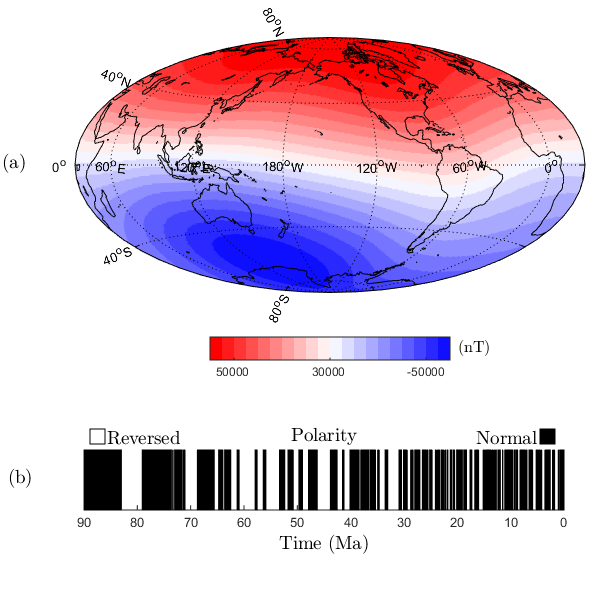
\includegraphics[scale=0.6]{Earth_Field.png}
\caption{(a) Dipolar magnetic field of the Earth in its normal orientation. (b) Polarity of the field inferred from the geological record over the past 90 Ma \cite[]{Cande1995}.}
\label{fig:Earth_Field}
\end{figure}

Natural Remanent Magnetization $\vec M_{NRM}$ is a permanent magnetization moment preserved in the absence of an inducing field.
The reader is encouraged to refer to \cite{Blakely96} and \cite{Clark99} for a more in-depth explanation of chemical, thermal and biological processes responsible for the remanent component of various rock types.
While the induced component is linearly related to the inducing field, nothing can be assumed about the NRM orientation and it remains challenging to estimate.
If aligned with the inducing field direction, the NRM is indistinguishable from a purely induced response, resulting in an over-estimation of the magnetic susceptibility of rocks.
For large NRM components, perpendicular or anti-parallel to the inducing field, the magnetic response of compact objects may get distorted, potentially resulting in false interpretation about the distribution and geometry of rock units.
Direct geological interpretation of magnetic data that ignores the effect of remanence has long been recognized as problem in mineral exploration.
This brings up an important question:
How can we better recover the location and geometry of magnetized objects without knowledge of the total magnetization direction $\vec M$?

From Gauss's law, the relation between the observed magnetic field and rock magnetization is expressed as:
\begin{equation} \label{b_integral}
	\vec b(r) = \frac{\mu_0}{4\pi} \int_{V} \nabla \nabla \frac{1}{ r} \cdot \vec M \; dV\;,
\end{equation}
where $\vec b$ is the magnetic field (T) as measured at some distance $ r$ from a magnetic anomaly with magnetization per unit volume $\vec M$ (A/m).
Since $\vec b$ is usually small, it is commonly measured in units of nano-Tesla (nT).
The majority of magnetic data consist of Total Magnetic Intensity (TMI) measurements which can be written as:
\begin{equation}
	b^{TMI} = |\vec B_0 + \vec B_A| \;,
\end{equation}
where we measure the magnitude of the field rather than the individual components.
In most cases we are only interested in the anomalous local fields.
Under the assumption that $|\vec B_A| \ll |\vec B_0|$, the anomalous field is approximated to be parallel with the direction of the inducing field $\hat B_0$.
The Total Magnetic field Anomaly (TMA) is given by:
\begin{equation}
\begin{split}
	b^{TMA} &= |\vec B_0 + \vec B_A| - |\vec B_0| \\
	&\simeq  \vec B_A \cdot \hat B_0 \;.
\end{split}
\end{equation}
Figure~\ref{fig:Magnetization} gives an example of TMA data measured on a plane above a magnetized sphere.
The main challenge in interpreting magnetic data is to characterize the magnetic sources when nothing is known about the location and magnetic properties ($\kappa,\;\vec M$) of buried objects.
Accurately imaging the location and geometry of magnetic objects is a core problem in exploration geophysics.


\begin{figure}[h!]
\centering
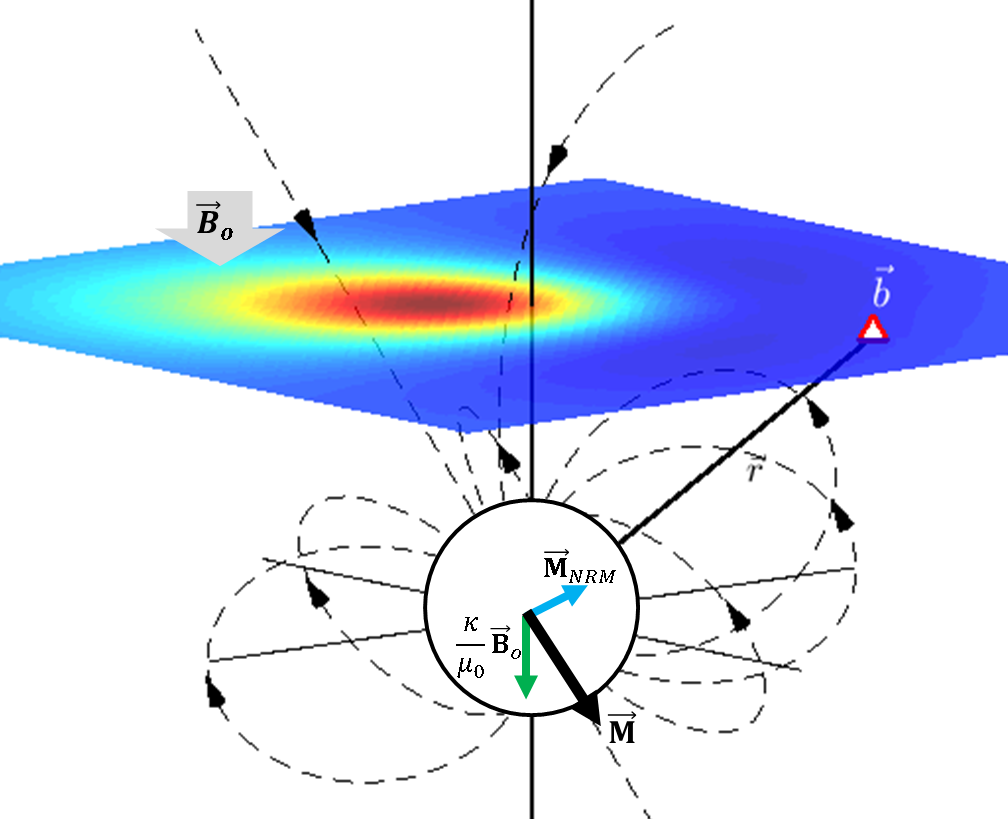
\includegraphics[scale=0.55]{Magnetization_EDT.png}
\caption{Magnetic field data $\vec b$ observed on a plane over a magnetized sphere located at the origin. The orientation and magnitude of magnetization of the sphere is function of the magnetic susceptibility $\kappa$, the inducing field $\vec B_0$ and remanent components $\vec M_{NRM}$, neglecting self-demagnetization effects. }
\label{fig:Magnetization}
\end{figure}

Early geophysical studies relied primarily on filtering techniques to infer geological structures and identify potential targets \cite[]{Cowan2000}.
In order to reduce the complexity of the problem, the magnetization direction is in most cases assumed to be purely induced along $\vec B_0$, neglecting self-demagnetization and remanence effects.
Inversion codes, such as the UBC-MAG3D from \cite{LiOldenburg1996}, also rely on this assumption.
While the induced component may dominate in most cases, recent petrophysical studies seem to indicate that the effect of remanent magnetization may be more important than previously thought \cite[]{Enkin2014}.
This is especially true for specific types of mineral deposits such as Banded Iron-Formations (BIF) and diamondiferous kimberlite \cite[]{Dransfield2003, LiShearer10}
Strong remanent magnetic components can hinder the interpretation of magnetic data thus leading to false drilling targets.

\section{Magnetic methods}
Several studies have been dedicated to the inversion of magnetic data in the presence of remanence.
As summarized by \cite{Li2012}, the proposed inverse methods can be divided into three categories.
The first category estimates the magnetization direction from the data in a pre-processing step.
Strategies such as the Helbig's method \cite[]{Phillips03} and the cross-correlation \cite[]{DannemillerLi06} are used upstream of standard inversion codes.
Adapted from the 2-D analytical signal of \cite{Nabighian72}, \cite{Roest92} estimate the orientation of remanence in 3-D.
In most cases, data are transformed to the wavenumber domain in order to extract magnetic field components.
These methods are simple and robust for simple and isolated anomalies, but become impractical when the data are acquired over rough terrain or complicated geology.

The second category deals with magnetic data that are weakly dependent on the orientation of magnetization.
It has been shown that magnetic amplitude data are weakly dependent on the magnetization direction in 3-D \cite[]{Nabighian72}.
Magnetic amplitude data are simply calculated as:
\begin{equation}
|\vec b| = {( b_x^2 + b_x^2 + b_x^2 )}^{1/2}\;,
\end{equation}
where $b_x$, $b_y$ and $b_z$ are the three components of the anomalous magnetic field.
Inverting magnetic amplitude data can provide a robust estimate for the location of magnetized bodies
as shown by \cite{Shearer05}. Magnetic amplitude data are successfully inverted over a kimberlite deposit, recovering the true location of kimberlite pipes and associated magnetic dykes.
Because most magnetic surveys only record TMI data, the three components of the field must be derived in post-processing.
Two strategies have been proposed in the literature to extract magnetic field components.
The first relies on the fact that magnetic data are potential field data, hence knowledge of any component of the field on an infinite plane above the source is sufficient to calculate the remaining components. 
Data are interpolated onto a uniform grid, which is then used to calculate the components of the field using Fourier transform techniques.
This may be a problem however for airborne surveys over steep topography or acquired at low latitude.
Alternatively, the equivalent-source method has been proposed by \cite{Li2010} to alleviate those constraints.
Taking advantage of the non-uniqueness of potential field data, TMA data are inverted for a layer of magnetic sources then used to forward model three-component magnetic data.


The third method directly solves for the orientation of magnetization without making any assumptions about the location or geometry of causative bodies.
In the Magnetic Vector Inversion (MVI) proposed by \cite{Lelievre2009}, the magnetization vector is decomposed in its induced and orthogonal components.
The MVI is closely related to the method proposed by \cite{Kubota2005}, and later borrowed by \cite{Ellis2012}.
This method results in a large under-determined inverse problem, with roughly three times the number of free-variables over conventional susceptibility inversion codes.
Recovered magnetization models are generally smooth and become overly complicated for direct geological interpretation.
As pointed out by \cite{PhDLelievre09}, any \emph{a priori} information from surface or borehole measurements may greatly reduce the non-uniqueness of the problem.
Unfortunately this kind of information is rarely available in greenfield settings or is only available in sparse samples.

Building upon the work of \cite{Shearer05}, \cite{Liu2015} propose a hybrid three-step process to invert for the location, orientation and magnetic susceptibility distribution in 2-D.
In the first step, the location of magnetic material is inverted from amplitude data.
Next, the orientation of magnetization is found via a correlation method.
The orientation of magnetization is then used in a standard inversion code to recover a susceptibility model.
The combined method greatly reduces ambiguity about the location and orientation of isolated targets, but becomes challenging over multiple anomalies with variable magnetization directions.
The same synthetic model was applied to the MVI method, resulting in a poor recovery for the location and intensity of magnetization.
This result is surprising considering the satisfactory solution obtained in previous studies \cite[]{Ellis2012, Lelievre2009}.
The combined approach of \cite{Liu2015} is interesting however, as it links together complementary algorithms.

\section{Thesis outline}
Following the same line of thought as \cite{Liu2015}, I propose a Cooperative Magnetic Inversion (CMI) algorithm that directly incorporates the amplitude inversion of \cite{Shearer05} into the MVI algorithm of \cite{Lelievre2009}.
Magnetic field amplitude data are computed from the Equivalent Source technique proposed by \cite{Li2010}, removing the need to grid the data.
Moreover, I introduce a Scaled Iterative Re-weighted Least Squares (S-IRLS) regularization method to recover blocky and sparse solutions.
My thesis is divided into the following chapters:

In Chapter~\ref{ch:Chap2_Forward} and \ref{ch:Chap3_Inverse}, I provide further details about rock magnetism and review the theory related to inverse problems in the context of exploration geophysics. I revisit three inversion codes from the literature: the magnetic susceptibility inversion from \cite[]{LiOldenburg1996}, the magnetic amplitude inversion from \cite{Shearer05}, and the Magnetic Vector Inversion (MVI) from \cite[]{PhDLelievre09}.
Each of these codes are tested on a synthetic example with complicated magnetization distribution.
I also review the equivalent-source method from \cite{Li2010}.

In Chapter~\ref{ch:Chap4_Mixed_Lpnorm_Regularization}, I introduce a mixed $l_p$-norm regularization function for the recovery of compact and sparse solutions, increasing the flexibility of current inversion codes.
The method uses a Scaled Iterative Re-weighted Least Squares (S-IRLS) formulation to approximate any $l_p$-norm penalties on the interval $0 \le p \le 2$.
Sparse constraints are applied on both the model and model gradients independently.
The mixed-norm regularization is implemented on the magnetic problem, and tested on an airborne magnetic dataset from the Tli Kwi Cho kimberlite complex, Northwest Territories.

In Chapter~\ref{ch:Chap5_Cooperative_Mag_Inversion_CMI}, I formulate a Cooperative Magnetic Inversion (CMI) method, combining the inversion codes presented in Chapter~\ref{ch:Chap3_Inverse} and \ref{ch:Chap4_Mixed_Lpnorm_Regularization}.
The algorithm is tested on the same synthetic example for comparison.

Finally in Chapter~\ref{ch:Chap6_Case_Study}, I apply the CMI algorithm to a large aeromagnetic data set over the Ekati Property, Northwest Territories.
I design a tiled inversion scheme to automate the inversion process and to reduce the computational cost.
Individual models are then merged back onto a global mesh for analysis.
A bulk estimate of magnetization direction is compared to values published in the literature.
The polarities of magnetization over 11 pipes are compared to the estimated age of emplacement.
The analysis is extended to various dyke swarms, providing regional geologic information.

The work presented in this thesis is significant for two reasons.
First, the mixed-norm regularization function introduced in Chapter~\ref{ch:Chap4_Mixed_Lpnorm_Regularization} can considerably improve the flexibility of inversion algorithms, not limited to potential field problems.
The S-IRLS method allows for a combination of sparse norms on the model and model gradients independently, granting access to a wider range of solutions than previously offered by globally convex functions.
%Future research will focus on the implementation of the S-IRLS on other geophysical inverse problems such as for gravity and electromagnetic data.

Secondly, it is the first time that both the amplitude inversion and MVI algorithms are combined in a cooperative inversion method in 3-D.
Structural information gained by the amplitude inversion is used directly to constrain the MVI algorithm, reducing the non-uniqueness of the solution.
From a practical standpoint, it is an automated process that streamlines the inversion workflow.
This, in turn, can reduce the overall time required to process magnetic data and promote the expansion of inversion methods in mineral exploration.
%Future research will focus on the implementation of a non-linear spherical formulation for the MVI, improving the flexibility of the algorithm.

\endinput



%% The following is a directive for TeXShop to indicate the main file
%%!TEX root = Thesis_Driver.tex
\graphicspath{{./../../Figures/}}
\chapter{Forward modeling of potential field data}
\label{Chapter2}
My goal is to characterize the sub-surface in terms of density and magnetization. In Chapter~\ref{Chapter1}, I have introduced the basic physics describing the relation between density and magnetization and their respective anomalous fields in integral form. In this chapter, I provide numerical details about the transformation from the continuous space to a discrete linear system of equations. I also provide efficiency improvements over conventional implementations for the processing of large scale data sets.

\section{Discrete systems}
The usual strategy is to represent the continuous Earth in terms of unit elements each contributing to the total response observed at a given position in space.
For the gravity problem, the integral in \eqref{g_integral} can be evaluated analytically over a discrete prism with uniform density $\rho$. As derived by \cite{Nagy66}, the integration gives rise to a linear system:
\begin{equation} \mathbf{g} = \begin{bmatrix} T_{x} \\ T_{y} \\ T_{z} \end{bmatrix} \; \rho \;, \label{gfield} \end{equation}
where $\mathbf{T}$ relates the cell-centered density value to the observed gravity field $\mathbf{g}$ at some location $P(x_P, y_P, z_P)$:
\begin{equation}
\begin{split}
T_{x} &= -G \bigg( \arctan \frac{dy\;dz}{r\:dx} + \log \left[\; dz + r\;\right] + \log \left[\; dy + r\;\right] \bigg) \bigg|_{x_L}^{x_U} \bigg|_{y_L}^{y_U} \bigg|_{z_L}^{z_U}\\
T_{y} &= -G \bigg( \arctan \frac{dx\;dz}{r\:dy} + \log \left[\; dz + r\;\right] + \log \left[\; dx + r\;\right] \bigg) \bigg|_{x_L}^{x_U} \bigg|_{y_L}^{y_U} \bigg|_{z_L}^{z_U}\\
T_{z} &= -G \bigg( \arctan \frac{dy\;dy}{r\:dz} + \log \left[\; dy + r\;\right] + \log \left[\; dy + r\;\right] \bigg) \bigg|_{x_L}^{x_U} \bigg|_{y_L}^{y_U} \bigg|_{z_L}^{z_U}\\
r &= (dx^2 + dy^2 + dz^2)^{1/2} \\
dx &= (x_P - x), \; dy = (y_P - y),\; dz = (z_P - z)\\
\end{split}
\label{Tmatrix}
\end{equation}
and $G$ is Newton's gravitational constant.
Parameters needed to define the position and shape of a unit cell are presented in Figure~\ref{UnitCube}. Only the lower southwest $L(x_L,y_L,z_L)$ and upper northeast $U(x_U,y_U,z_U)$ corner coordinates are needed to define the relative distance $\mathbf{r} (dx,\:dy,\:dz)$ between the observation point and the nodal limits. In this research I use right-handed Cartesian coordinate system such that the $\hat x$, $\hat y$ and $\hat z$ coordinate axes point along the east, north and vertical (up) direction respectively.
\begin{figure}[h!]
\centering{
\includegraphics[width=0.55\columnwidth]{PF_UnitCube.png}}
\caption{Parameters describing the spatial relationship between an observation point $P$ and a rectangular prism $C$.}
\label{UnitCube}
\end{figure}

For most gravity field experiments only the vertical component of field $g_z$ is measured, such that \eqref{gfield} reduces to
\begin{equation}
\begin{split}
g_z =\;& {T}_z \;{\rho} \\
\end{split}\label{g_discrete}
\end{equation}
Equation~\eqref{g_discrete} defines the gravity response of a single rectangular prism as observed at a single position in space. I can augment equation \eqref{g_discrete} to describe a gravity experiment conducted over a large volume of earth and at many observation stations
\begin{equation}\label{g_discrete_large}
	\mathbf{g}^{pre} = \mathbf{G} \boldsymbol{\rho}
\end{equation}
such that the linear forward operator $\mathbf{G}\in \mathbb{R}^{N\times M}$ maps the contribution of $M$ number of prisms ($\boldsymbol{\rho} \in \mathbb{R}^M$), each contributing to the response measured over $N$ observation locations ($\mathbf{g}^{pre} \in \mathbb{R}^{N}$).
There are many ways to organize the cells making up this discrete model.
In all the work presented in this thesis, I use an Octree-based discretization.
More details regarding this choice of parameterization are provided in the following section.

Similarly for the magnetic response, the integral equation in \eqref{b_integral} can be evaluated analytically for a single prism \cite[]{Sharma66}. This gives rise to a linear system of the form
\begin{equation}\label{b_discrete}
\begin{split}
	\mathbf{b} = \mathbf{T} \mathbf{m} \;,
\end{split}
\end{equation}
where $\mathbf{T}$ is a dense 3-by-3 symmetric matrix describing the linear relation between a prism with magnetization $\mathbf{m} = [M_x,\;M_y,\;M_z]^T$ to the components of the field $\mathbf{b} = [b_x,\;b_y,\;b_z]^T$.
\begin{equation}
\begin{split}
\mathbf{T} & = \frac{\mu_0}{4\pi} \begin{bmatrix} T_{xx}& T_{xy}& T_{xz} \\T_{xy} & T_{yy} & T_{yz} \\ T_{xz}&T_{yz} & T_{zz} \end{bmatrix} \\
\end{split}
\label{Tmatrix}
\end{equation}
where $\mu_0$ is the magnetic permeability of free-space. It is important to note that the tensor $\mathbf{T}$ is a symmetric matrix with zero trace. Therefore only five of the nine tensor components need to be calculated.
\begin{equation}
\begin{split}
T_{xx} &= -\arctan \frac{dx\;dy}{{dx}^2 + r\:dz + {dz}^2} \bigg|_{x_L}^{x_U} \bigg|_{y_L}^{y_U} \bigg|_{z_L}^{z_U} \\
T_{yy} &= -\arctan \frac{dx\;dy}{{dy}^2 + r\:dz + {dz}^2} \bigg|_{x_L}^{x_U} \bigg|_{y_L}^{y_U} \bigg|_{z_L}^{z_U} \\
T_{xy} &= \log \left[\; dz + r\;\right] \bigg|_{x_L}^{x_U} \bigg|_{y_L}^{y_U} \bigg|_{z_L}^{z_U}\\
T_{xz} &= \log \left[\; dy + r\;\right] \bigg|_{x_L}^{x_U} \bigg|_{y_L}^{y_U} \bigg|_{z_L}^{z_U}\\
T_{yz} &= \log \left[\; dx + r\;\right] \bigg|_{x_L}^{x_U} \bigg|_{y_L}^{y_U} \bigg|_{z_L}^{z_U}\\
%T_{zz} &= -\arctan \frac{dx\;dy}{r\:dz} \bigg|_{L_x}^{U_x} \bigg|_{L_y}^{U_y} \bigg|_{L_z}^{U_z} \\
\end{split}
\end{equation}


For most geophysical applications, we do not measure the vector field $\vec b$, but rather the Total Magnetic Intensity (TMI) of the field that includes both the geomagnetic and secondary fields. Since we are only interested in the anomalous response from rocks, the approximation is generally made that
\begin{equation}\label{TMIprojection}
{b}^{TMA} = \vec{b} \cdot {{\hat H_0}} - \mu_0\|\vec{H}_0\|;
\end{equation}
such that the Total Magnetic Anomaly $b^{TMA}$ is assumed to be small and parallel to Earth's field $\vec{H}_0$.
The simulated magnetic datum in \eqref{b_discrete} simplifies to
\begin{equation}
\begin{split}
{b}^{pre} =\; \left[ \mathbf{ {\hat H}}_0^\top \cdot \mathbf{T}\right]\;\mathbf{m}
\end{split}
\end{equation}
Just as for the gravity experiments, this system can be augmented for $M$ number of prisms ($\mathbf{m} \in \mathbb{R}^{3M}$) and $N$ observation locations ($\mathbf{b}^{pre} \in \mathbb{R}^{N}$)
\begin{equation}\label{magLinearOpt}
\mathbf{b}^{pre} =\; \mathbf{F} \;\mathbf{m}
\end{equation}
such that $\mathbf{F}\in \mathbb{R}^{N\times 3M}$. This linear system has three times the number of parameters compared to the gravity problem as magnetization is a vector property.
As part of my contribution to the open-source community, both the gravity and magnetic kernels have been added to the \texttt{SimPEG.PF} library.

\subsection{Choice of discretization}
I have so far established the linear equations \eqref{g_discrete_large} and \eqref{magLinearOpt} that map the gravity and magnetic response for a collection of rectangular prisms making up a discrete Earth. I have yet to define how these cells are organized in a 3D space. This decision will directly affect the size of the forward (and later inverse) calculations as the size of the linear operators scale linearly with respect $M$. Approximating the Earth more efficiently will allow me to process large data sets.

The usual strategy is to define a core region of interest with a fine discretization and surround it by coarser cells (padding) to absorb regional signals that may be present in the data.
Two options are available to organize rectangular prisms.
The simplest implementation uses a regular grid, or tensor mesh shown in Figure~\ref{MeshType}(a). Each unit element shares a face with 6 neighbours. Changes in cell size propagate throughout the domain along the orthogonal direction. The use of tensor meshes has dominated the inversion literature due to the ease of storing and viewing uniformly gridded models.
\begin{figure}[h!]
{\centering
\includegraphics[width=\columnwidth]{MeshType.png}}
\caption{Simple representation of (a) tensor and (b) Octree meshes for the organization of rectangular prisms within a core domain (red) and padding region over a square domain 4 x 4 m in width. The Tensor mesh can fill the space with 64 cells, compared to only 40 cells with the Octree mesh.}
\label{MeshType}
\end{figure}

In an Octree mesh, unit cells are organized in a hierarchical structure as shown in Figure~\ref{MeshType}(b). The resolution of the grid is increased by dividing a parent cell into 8 children (or 4 in 2D). This type of discretization offers the most flexibility for increasing the resolution of the mesh in a specific region without affecting the resolution of boundary cells.
The main challenge is in generating a mesh that honours the geometry of the problem in terms of data location, topography and geological contacts.
Over the course of my research, I contributed to the open-source community with a suite of refinement functions to facilitate the creation process of Octree meshes.
As part of the \texttt{SimPEG.discretize} library, I implemented the following three strategies:
\begin{itemize}
\item Box refinement includes all cells intersected by a rectangular box containing the input points.
\item Radial refinement is performed inside spheres centered on each input points. The radial distance is determined by the user.
\item Surface refinement is defined by a continuous Delaunay triangulation of the input points \cite[]{Barber1996}. The Octree refinement is determined based on the vertical distance between cell centers and the nearest triangle. 
\end{itemize}
Figure~\ref{Refinements} compares the three refinement methods for the discretization of points (red) placed on a  Gaussian surface. The \texttt{box} refinement is the simplest but also the least efficient strategy as it yields a uniform grid similar to the Tensor discretization. For the \texttt{radial} refinement, I end up with a small number of cells concentrated around the input points. It is an optimal refinement for scattered observation points. The \texttt{surface} is well suited to describe continuous features such as topography and geological contacts. It gives, in this case, the most accurate representation of the Gaussian surface.
\begin{figure}[h!]
{\centering
\includegraphics[width=\columnwidth]{Refinements.png}}
\caption{Three refinement strategies used to discretize a Gaussian curve defined by scattered points (red): (a) \texttt{box}, (b) \texttt{radial} and (c) \texttt{surface} refinement strategy from the \texttt{SimPEG.discretize} library. Cells are coloured by their corresponding Octree level.}
\label{Refinements}
\end{figure}

\subsubsection{Forward simulation test}
I demonstrate the benefit of an Octree discretization by forward modelling the response of a 1 m sphere shown in Figure~ \ref{Discretization}. I want to compare the numerical cost to perform forward simulations using the standard Tensor discretization and an Octree mesh with \texttt{surface} refinement.
Octree refinement uses scatter points placed on the outer surface of the sphere. Using equation \eqref{b_discrete}, I calculate the magnetic response over an 11-by-11 grid of observations placed 1 m above the anomaly. I repeat the forward simulation over a range of cell sizes. Only cells inside the sphere are considered.
The forward calculations are compared to the analytical vertical response ($b_z^{ana}$) for a vertical magnetization:
\begin{equation}
b_z^{ana} = \frac{\mu_0}{4\pi}\left[ -\frac{{\bf M}}{r^{\,3}} + \frac{3\,({\bf M}\cdot{\bf r})\,{\bf r}}{r^{\,5}} \right] \cdot \hat z
\end{equation}
where $\mathbf{M}=[0\:\hat x\;, 0\:\hat y,\; 1\:\hat z]$ and $\mathbf{r}$ defines the vector between the center of the sphere and the observation location.
Table~\ref{AnalyticSphere} summarizes the forward calculations in terms of total number of cells, run time and data residual between the simulation and the analytic solution.
\begin{equation}\label{dataResidual}
\phi_d = \sum_{i=1}^{121} (b_{i} - b_{i}^{ana})^2
\end{equation}
All calculations were performed on a single thread 2.4 GHz Intel processor.
\begin{figure}[h!]
{\centering
\includegraphics[width=\columnwidth]{Discretization.png}}
\caption{(a) Discretization of a sphere defined by discrete points (red) using the conventional Tensor mesh with a core region and padding cells. Octree meshes refined by (b) \texttt{box}, (c) \texttt{radial} and (d) \texttt{surface} methods from the \texttt{SimPEG.discretize} library. }
\label{Discretization}
\end{figure}

For the Tensor mesh, a reduction in core cell size increases the total number of cells by a factor 8. For the same reduction in cell size using the surface refinement increases the number of cells by a factor 4. This is anticipated as only cells at the surface of the sphere decrease in size compared to a full volume refinement in the Tensor mesh. Both discretizations can reproduce the analytical response with roughly the same accuracy. Including padding cells to this problem would further increase the efficiency gap between the two discretization methods as the Octree mesh can rapidly increase the cell size with little influence from the discretization in the core region.
\begin{table}\centering
\begin{tabular}{|c|c|c|c||c|c|c|}\hline
& \multicolumn{3}{c}{Tensor} \vline \vline & \multicolumn{3}{c}{Octree (Surface)}\vline \\ \hline
Cell size (m) & \# Cells & Time (s) & $\phi_d$ & \# Cells & Time (s) & $\phi_d$ \\ \hline
1.00e-01 & 544 & 1.8e-01 & 4.2e+02 & 496 & 1.6e-01 & 7.7e+02 \\
5.00e-02 & 4196 & 9.6e-01 & 4.7e+01 & 2516 & 5.1e-01 & 7.1e+01 \\
2.50e-02 & 33478 & 6.5e+00 & 4.2e+00 & 10836 & 2.1e+00 & 5.2e+00 \\
1.25e-02 & 268080 & 6.5e+01 & 2.0e+00 & 47276 & 1.0e+01 & 2.7e+00 \\
\hline
\end{tabular}
\caption{Summary table for the forward modeling of a magnetized sphere using a Tensor and Octree discretization}
\label{AnalyticSphere}
\end{table}


\section{Large scale problems}\label{MeshDecoupling}
The amount of memory needed to store the dense linear operators for gravity and magnetics is a limiting factor for the simulation of potential field data with the integral formulation. As prescribed in \eqref{magLinearOpt}, the size of the problem is linearly scaled by the number of model parameters $M$ and the number of the data $N$. For moderate size problems encountered in exploration geophysics ($M\approx 10^6$, $N\approx10^4$) the memory requirement to store a dense $M\times N$ matrix can exceed hundreds of gigabytes. While modern supercomputers can handle problems of this size, it is still out of reach for common desktop computers.

A number of strategies have been proposed in the past to reduce the size of the problem. Compression methods, either in the Fourier \cite[]{Pilkington97} or wavelet domain \cite[]{LiOldenburg03}, have proven successful in reducing the size of the forward operators. On the downside, compression methods are prone to introducing modelling artifacts, which can be hard to differentiate from true anomalies. This is especially an issue for the magnetic vector inversion explored in Chapter~\ref{Chapter3}.

Another group of methods takes advantage of the rapid decay of geophysical signals to reduce the size of individual forward simulations. The assumption is made that model parameters in the far-field of measurements contribute little to the total response and can, therefore, be approximated with fewer parameters. In this regard, the concept is loosely related to the Fast Multipole Method \cite[]{Engheta1992}. This is especially valid for airborne EM experiments where cells beyond roughly 10 times the flight height of airborne EM systems have a negligible impact on the measured response \cite[]{Reid2006}. In its simplest implementation, \cite{Cox2010} define a footprint approach such that model parameters outside a pre-defined tolerance are simply ignored.

More recently, \cite{Yang2014} introduced a mesh decoupling approach. Local meshes are designed based on the source location and decay rate of the geophysical signal. Cell-centered conductivity values are homogenized using volumetric-weighted averaging. Similarly, \cite{Haber2014} designed a nested Octree mesh strategy. The core region of local meshes is co-located with cells in the global mesh and cover the same lateral extent. Physical property values are homogenized from small cells in the global mesh to larger (or equal) cells in the local meshes. This strategy assures that far-field features can still contribute to the total response. The accuracy of individual forward simulations depends primarily on the interpolation scheme used to transfer physical properties from the global to the local meshes.

In this research, I employ the methodology of \cite{Haber2014}. I want to divide the full data set into subsets (or tiles), each associated with a local mesh. Physical property values are transferred to local meshes using a volumetric weighted average. In order to further minimize the memory footprint of the simulation, I make use of the parallel \texttt{Dask} package \cite[]{dask2016}. The library was designed by the data science community for out-of-core processing of large datasets \cite[]{Scipy2015}. The \texttt{zarr} file format allows the storage of dense arrays on a solid-state drive (SSD) in compressed memory chunks. Out-of-core storage is appealing as it reduces the amount of Random-Access Memory (RAM) needed to store the large forward operators. Read and write operations are done in parallel. The runtime depends largely on the hardware used in terms of processor speed, number of processors and communication speed between the workers and the solid-state memory. The size of individual memory chunks can be adjusted to optimize the processing speed depending on the resources available.

In the case of potential field data, the source of geophysical signals can span a broad range of wavelengths, from tens of meters (local) to hundreds of kilometres (regional). The memory footprint of a problem can be reduced considerably if we manage to approximate far-field features with fewer cells. In the most extreme case, each observation point could have its own local mesh.
Choosing the number of tiles becomes a trade-off between accurately capture the heterogeneity of the model for forward modeling while minimizing traffic between the parallel workers and the SSD memory.

\subsection{Numerical test}
I investigate this trade-off between accuracy and efficiency with a numerical example.
I create a synthetic gravity model shown in Figure~\ref{Tiled_Test_model}. The model contains both short wavelength information from a small block anomaly and long wavelength signal from large domains in the north and southeast quadrants. From equation \eqref{g_discrete_large}, I compute gravity data on $21 \times 21$ grid placed 1 m above a flat topography.
Forward simulation of the global model required 4.3 Mb of memory and was performed in parallel in 6.7 s with 4 processors (2.4 GHz). It is a relatively small example compared to industry standards, but similar trends are to be expected on larger scale problems.
\begin{figure}[h!]
{\centering
\includegraphics[width=\columnwidth]{Tiled_Test_model.png}}
\caption{(a) Horizontal and (b) vertical sections through the synthetic density model used to test the mesh decoupling strategy. (c) The simulated data contain short and long wavelength information.}
\label{Tiled_Test_model}
\end{figure}

I will assess the trade-off between efficiency and numerical accuracy by performing a series of five forward simulations using a range of tiling patterns. I break up the dataset into 2, 4, 9, 12 and 16 square tiles.
For each tiling experiment, I calculate the total memory footprint (Gb) and the computation time (s) to perform the forward simulations. I also compute the data residual between the global simulation (single mesh) and the tiled simulation using the $\ell_2$-norm measure in equation \eqref{dataResidual}.
\begin{figure}[h!]
{\centering
\includegraphics[width=\columnwidth]{Tiled_Dask.png}}
\caption{Example of mesh decoupling of the forward problem into nested Octree tiles. (Middle) Local meshes are generated for a pre-defined number of tiles nested inside the global domain. (Bottom) The forward modelling operator for each tile is stored in compressed \texttt{Zarr} file format on solid-state memory. Memory chunks (grey) are accessed in parallel by the \texttt{Dask} library to perform the forward calculations.}
\label{Tiled_Dask}
\end{figure}

As seen in Figure~\ref{Tiled_Test_Size}, the memory needed to perform the forward calculations rapidly decreases but eventually levels-off as the number of tiles increases. This is expected as local meshes necessitate a minimum number of cells to fill out the global domain and a minimum number of small padding cells near the edge of the tiles to reduce interpolation artifacts. The reduction in problem size is inversely correlated with an increase in computational time as communication between the workers and the SSD memory becomes a bottleneck.
\begin{figure}[h!]
{\centering
\includegraphics[width=\columnwidth]{Tiled_Test_Size.png}}
\caption{Trade-off curves between the size of the forward problem (blue) and data residual (red) over a range of number of tiles. The total size of the problem is calculated based on the sum of cells in all the local meshes times the number of data. The optimal number of tiles would be at the point of intersection where both the cost of forward calculations and the data residual change significantly.}
\label{Tiled_Test_Size}
\end{figure}

I also note an increase in data residual as a function of tile size.
Figure~\ref{Tiled_Residual} compares the simulated data from the global mesh (single tile) to the combined forward simulation calculated with 12 tiles (last experiment). From the residual map, it is possible to distinguish short wavelength discrepancies between adjacent forward simulations (tiles). These residuals are primarily due to the homogenization of anomalies near the edges of tiles, which in turn is a function of the wavelength information contained in the data. As a first pass, I establish experimentally the appropriate padding distance based on the estimated data uncertainties, such that the maximum residual falls below the experimental error. For this experiment, the meshing artifacts are at most $2\%$ of the data amplitude (or 0.004 mGal), which I achieved with a minimum padding distance of 4 cells per Octree level. Determining an optimal padding distance as a function of the geophysical signal would warrant further research. 
\begin{figure}[h!]
{\centering
\includegraphics[width=\columnwidth]{Forward_Tiles.png}}
\caption{Simulated gravity data calculated from (a) the global model and (b) the 12 forward tiled calculations. (c) Data residuals show short wavelength discrepancies between adjacent tiles due to interpolation effects.}
\label{Tiled_Residual}
\end{figure}


\endinput



%% The following is a directive for TeXShop to indicate the main file
%%!TEX root = Thesis_Driver.tex
\graphicspath{{./../../Figures/}}
\chapter{Inverse Problem}
\label{Chapter3}
In Chapter~\ref{Chapter2}, I defined the linear equations relating density and magnetization to gravity and magnetic data. I now review the theory needed to solve the inverse problem, such that I can recover a 3D representation of the subsurface from the observed data.
A key issue related to the inverse problem is that there is an infinite number of
possible models that can satisfy the data. Field measurements are generally acquired from the surface resulting in the inverse problem to be ill-posed. The presence of experimental noise further complicates the problem.
To circumvent these issues, the inversion is often formulated as an optimization problem of form
\begin{equation}
\begin{split}\label{GenMinProb}
\underset{\mathbf{m}}{\text{min}}\; \phi(m) & = \; \phi_d + \beta \phi_m \\
\text{subject to} \; \phi_d & \leq \phi_d^* \; .
\end{split}
\end{equation}
where $\phi_d$ is the misfit function
\begin{equation}\label{eq:misfit}
\phi_d =\sum_{i=1}^{N}\left(\frac{d_i^{pred} - {d}_i^{obs}}{\sigma_i}\right)^2 \;,
\end{equation}
that measures the residuals between the observed and predicted data $\mathbf{d}^{pre}$, normalized by the estimated data uncertainties $\boldsymbol{\sigma}$.

The regularization function $\phi_m$, or model objective function, serves as a vehicle to introduce \emph{a priori} information in the inversion.
Several regularization strategies have been developed over the last decades such that the solution remains geologically plausible.
I focus on the generic $\ell_p$-norm regularization of the form
\begin{equation}
\begin{split}\label{intSmall}
\phi_m &= \sum_{r=s,x,y,z} \alpha_r \int_V w(m) |f_r (m)|^{p_j} \;dV\;. \\
\end{split}
\end{equation}
The functions $f_r$ can take many forms but most often have been
\begin{equation}
\begin{split}\label{fj}
f_s= m-m^{ref},\;f_x= \frac{d m}{dx},\; f_y= \frac{d m}{dy},\;f_z= \frac{d m}{dz}\;.
\end{split}
\end{equation}
Thus $f_s(m)$ measures the deviation from a reference model $m^{ref}$ and $f_x(m)$, $f_y(m)$ and $f_z(m)$ measure the roughness of the model $m$ along orthogonal directions in 3D.  
This optimization problem has multiple terms scaled by hyper-parameters. The first parameter is $\beta$ which controls the balance between misfit and regularization. It is assumed that a value can be found such that the target misfit is reached.
The $\alpha$'s are constants that control the relative influence of the different regularization functions. A larger $\alpha$-value increases the focus of the optimization on the corresponding penalty function.
User-defined weights $w(m)$ are used to incorporate any type of \emph{a priori} information that may be available to guide the solution.
 
Most often the $\ell_2$-norms measure has been used giving rise to a discrete linear system of form
\begin{equation}\label{leastSquaresLin}
\begin{split}
\phi_m &= \alpha_s \phi_s + \alpha_x \phi_x +\alpha_y \phi_y+\alpha_z \phi_z\\
& = \sum_{r=s,x,y,z} \alpha_r \|\mathbf{W}_r \;\mathbf{V}_r \;\mathbf{G}_r \;(\mathbf{m}-\mathbf{m}^{ref})\|_2^2 \;,\\
\end{split}
\end{equation}
where $\phi_s$ measures the deviation of the discrete model $\mathbf{m}$ from a reference model $\mathbf{m}^{ref}$ and $\phi_x$, $\phi_y$ and $\phi_z$ measure the roughness of the model along Cartesian directions. The reference model is sometimes omitted in the roughness terms. The matrices $\mathbf{G}_x,\;\mathbf{G}_y,$ and $\mathbf{G}_z$ are discrete gradient operators. 
For the smallness component, $\mathbf{G}_s$ reduces to the identity matrix. Volumes of integration resulting from the evaluation of \eqref{intSmall} are applied through diagonal matrices such that 
\begin{equation}
\mathbf{V}_s = diag\left[ \mathbf{v}^{1/2}  \right]\;.
\end{equation}
where $\mathbf{v}$ holds the discrete volume elements corresponding to each cell.
For the model derivative terms, the volume of integration is computed over cell interfaces such that
\begin{equation}\label{volumeAve}
\mathbf{V}_x = diag\left[\left( \mathbf{A}_C^{F_x} \mathbf{v}\right)^{1/2}  \right]\;.
\end{equation}
where the matrix $\mathbf{A}_C^{F_x}$ averages the cell-centered volumes to cell faces. Similar averaging is performed along the orthogonal $y$ and $z$-direction. Diagonal matrices $\mathbf{W}_r$ hold user-defined weights. More details about these weights are provided in the following section. 
Lastly, the $\alpha$ parameters control the relative importance given to individual components of the regularization.
What is sometimes sought, at least as a first pass, is that if $\phi_s$, $\phi_x$, $\phi_y$, $\phi_z$ have about the same numerical value then they are contributing equally. Dimensional analysis shows that for a uniform discretization $h$:
\begin{equation}\label{lengthScale}
\frac{[\phi_x] }{ [\phi_s]} = {[h]}^{-2}\;.
\end{equation}
The common approach is to set $\alpha_s$ accordingly in order to scale the components of the regularization function.

The usual strategy to solve \eqref{GenMinProb} is through a gradient descent algorithm, such as a Gauss-Newton approach, where we attempt to find a solution that has zero gradients
\begin{equation}\label{gradPhi}
\mathbf{g} = \nabla_m \phi(\mathbf{m}) = \nabla_m \phi_d + \beta \bigg[ \alpha_s \nabla_m \phi_s + \alpha_x \nabla_m \phi_x + \alpha_y \nabla_m \phi_y + \alpha_z \nabla_m \phi_z \bigg] = \mathbf{0} \;.
\end{equation}
where $\nabla_m$ stands for the partial derivatives of the function with respect to the discrete parameterization $\mathbf{m}$.
A solution to \eqref{gradPhi} can readily be calculated by gradient descent methods \cite[]{HestenesStiefel1952, NocedalWright99}.

A large number of studies have made use of this formulation to incorporate a variety of \emph{a priori} information: physical property data from rock and core samples \cite[]{LelievreOldenburgWilliams09}, structural knowledge \cite[]{LiDWO2000, PhDLelievre09} and advanced 3D geological modeling (\cite[]{Phillips1996, Williams08, Bosh2001, Fullagar2008}.
Although successful in identifying imaging anomalies at depth, penalty functions that rely on $\ell_2$-norm measures have a limited range of possible outcomes. The models tend to be smooth and difficult to interpret in relation to known geological domains with discrete boundaries. Moreover, substantial modelling work is generally required by experts to manually refine these constraints in order to test different geological scenarios.

\subsubsection{Sensitivity weighting}
The weighting matrices $\mathbf{W}_r$ introduced in \eqref{leastSquaresLin} can take many forms depending on the type of \emph{a priori} information that may be available. For potential fields problems, a sensitivity weighting function is generally used to counteract the rapid decay of the geophysical signal as a function of distance. In the work of \cite{LiOldenburg1996}, a \emph{distance weighting} approximation is employed and fixed at the onset.
In this thesis, I resort to an iterative re-weighting strategy based on the sensitivity of a given inverse problem
\begin{equation}\label{Jk}
\mathbf{J} = \frac{\partial \; F[\mathbf{m}]}{\partial \boldsymbol{\mathbf{m}}}\;,
\end{equation}
where $\mathbf{J}$, also referred to as the Jacobian matrix, holds the partial directives of the forward problem $F[\mathbf{m}]$ with respect to $\mathbf{m}$.
Adapted from \cite{Haber1997}, I formulate the sensitivity-based weighting function:
\begin{equation}\label{iter_sens_weight}
\begin{split}
\mathbf{W}_s &= \rm{diag} \left[ {\left[\frac{\mathbf{ w}}{\rm{max}(\mathbf{ w})}\right]}^{1/2}\right]\\
%\mathbf{\hat w}_r &= \frac{\mathbf{ w}_r}{max(\mathbf{ w}_r)}\\
w_{j} &= {\left[\sum_{i=1}^{N}{J_{ij}}^2 + \delta \right]}^{1/2} \Big/ v_j\;,
\end{split}
\end{equation}
where $\mathbf{w}$ measures the sum square of the columns of the Jacobian, normalized by the cell volumes. The constant $\delta$ is a small value (near machine precision) added to avoid singularity. The weights are normalized by the maximum value such that the range of weights are bounded between [0, 1]. 
The same sensitivity weights can also be applied to the model derivative terms using a cell averaging operation such that
\begin{equation}\label{sensWAve}
\mathbf{W}_x = diag\left[\left( \mathbf{A}_C^{F_x} \left[\frac{\mathbf{ w}}{\rm{max}(\mathbf{ w})}\right]\right)^{1/2}  \right]\;,
\end{equation}
similar to the averaging of volumes used in \eqref{volumeAve}. 
This sensitivity weighting strategy is general and adaptable to any inverse problems where the sensitivity matrix can be calculated explicitly.
While the initial purpose of the sensitivity weighting function of \cite{LiOldenburg1996} is to simply counteract the decay of potential fields, I will show numerically in Chapter~\ref{Chapter4} that the iterative re-scaling process can also be beneficial in improving the convergence of gradient methods applied to non-linear inverse problems.


\subsection{Synthetic gravity example}
As an entry point to the inverse problem, I proceed with a simple synthetic gravity example. I define a volume of interest 600 m wide by 300 m deep, over which I place a uniform survey grid of 21 x 21 stations placed 5 m above a flat topography.
The core region directly below the survey grid is discretized at a 5 m resolution as shown in Figure~\ref{GRAV_model}(a)
Within the core region, I build a geophysical target made up of a single dense cube, 25 m in width. I set the density contrast of the prism to 0.2 g/cc in a uniform zero background. From \eqref{g_discrete}, I simulate the vertical gravity field of the block and add random Gaussian noise with $10^{-3}$ mGal standard deviation. Figures~\ref{GRAV_model}(b) and (c) display the simulated data and `noisy' observations $\mathbf{g}_z^{obs}$ used in the inversion. I revisit this example in Chapter~\ref{Chapter4} to demonstrate the inversion process on magnetic data.
\begin{figure}[h!]
{\centering
\includegraphics[width=\columnwidth]{GRAV_Synthetic_True_data_model.png}}
\caption{(a) Vertical section through a 25 m cube with density $\rho$=0.2 g/cc placed in a uniform zero density background. (b) Simulated gravity data responses on a $21 \times 21$ survey grid placed 5 m above the flat topography. (c) Gravity data with random Gaussian noise added, $10^{-3}$ mGal standard deviation.}
\label{GRAV_model}
\end{figure}

From the noisy data I will attempt to recover the block anomaly by the inverse process. The objective function to be minimized takes in this case the form:
\begin{equation}
\begin{split}
\underset{\mathbf{m}}{\text{min}}\; \phi(m) & = \; \|\mathbf{G}\;\boldsymbol{\rho} - \mathbf{d}^{obs}\|_2^2 + \beta \sum_{r=s,x,y,z} \alpha_r \|\mathbf{W}_r \mathbf{V}_r \;\mathbf{G}_r \;\boldsymbol{\rho}\|_2^2 \\
\text{subject to} \; \phi_d & \leq \phi_d^* \;
\end{split}\label{gravLineObjFun}
\end{equation}
where I set $\boldsymbol{\rho}^{ref}=\mathbf{0}$.
Since \eqref{gravLineObjFun} is linear with respect to the density contrast model $\boldsymbol{\rho}$, I can solve it uniquely for a fixed trade-off parameter $\beta$. I repeat this process for variable $\beta$ values until a find a solution that satisfies $\phi_d \approx N$. 
Figure~\ref{Grav_l2model}(a) presents a vertical section through the recovered density model. The density anomaly is imaged at roughly the right position, but the edges of the block are poorly defined. As normally obtained with $\ell_2$-norm penalties, the solution is smooth and density values remain near the zero reference model. Hence the need to explore other regularization functions that can better resolve compact objects.
\begin{figure}
\includegraphics[width=\columnwidth]{Grav_Inv_l2model.png}
\caption{(a) Vertical section through the inverted density model using the conventional $\ell_2$-norm regularization, (b) predicted and (c) normalized data residual. Outline of the true model (red) is shown for reference.}
\label{Grav_l2model}
\end{figure}


\section{General $\ell_p$-norm regularization}
Alternatively, researchers have explored the use of non-$\ell_2$ measures to promote the recovery of compact anomalies. Approximations to $\ell_1$-norm such as the Huber norm \cite[]{Huber64}
\[
\sum_{i} {|m_i|}^p \approx \sum_{i} \left\{\begin{array}{lr}
m_i^2, & |m_i| \leq \epsilon,\\
2\epsilon|m_i|-\epsilon^2, & |m_i| > \epsilon,
\end{array}\right\}
\]
and the Ekblom norm \cite[]{Ekblom73}:
\begin{equation}\label{Ekblom}
\sum_{i} {|m_i |}^p \approx \sum_{i} {(m_i^2 + \epsilon^2)}^{p/2} \;
\end{equation}
have received considerable attention in geophysical inversion and signal processing \cite[]{Li93, Gorodnitsky97, FarquharsonOldenburg98, Daubechies10, SunLi14}.
Likewise, the Lawson's measure \cite[]{Lawson61}
\begin{equation}\label{eq:IntegralIRLS}
\begin{split}
	\sum_{i} {|m_i |}^p \approx \sum_{i} {\frac{ {m_i}^2}{\left( {{m_i}}^{2} + \epsilon^2 \right)^{1-p/2 }}} \;,	
\end{split}
\end{equation}
has been proposed to approximate $\ell_0$-norm and it has proven useful in generating minimum support models. This formulation has received considerable attention in the literature. \cite[]{Portniaguine1999, LastKubik83,BarbosaSilva94, Ajo-Franklin07}.
Figure~\ref{NormIRLS} compares the $\ell_p$-norms with the Lawson approximation over a range of model values. As $\epsilon \rightarrow 0$, the approximation approaches the $\ell_p$-norm on the complete interval $p \in [0, 2]$.
While \eqref{eq:IntegralIRLS} would in theory permit us to explore a wide range of solutions for $0\leq p\leq 2$, its numerical implementation remains challenging. Most algorithms have been limited to the $\ell_0$, $\ell_1$, and $\ell_2$-norm measure applied evenly to all components of the model objective function.
\begin{figure}
\includegraphics[width=\columnwidth]{NormIRLS.png}
\caption{Approximated $\ell_p$-norm using the Lawson measure \cite[]{Lawson61} over a range of $p$-values and for a fixed threshold parameter $\epsilon=10^{-1}$.}
\label{NormIRLS}
\end{figure}

Recent efforts by \cite{SunLi14} have shown promise in further exploring the model space by varying $\ell_p$-norm measures locally. They divided the inversion domain into regions reacting favourably to either the $\ell_1$ or $\ell_2$-norm regularization. The automated process could adapt to complex geological scenarios where both smooth and blocky anomalies are present.
Building upon the work I introduced in my M.Sc. Thesis \cite[]{Fournier2015}, I want to extend the work of \cite{SunLi14} and further generalized the mixed norm inversion for $p \in [0\;2]$.

\subsection{Synthetic 1D problem}
To develop my methodology it suffices to work with a simple test example.
In Figure~\ref{Problem1D}(a) I present a synthetic 1D model made up of a boxcar anomaly. The region is divided into 50 uniform cells distributed along the interval $[0 \le x \le 1]$. I define a synthetic geophysical experiment such that the data ($\mathbf{d}^{obs}$) are
\begin{equation}\label{Forward_Noisy}
\mathbf{d}^{obs} = \mathbf{F\;m}^{true} + \mathbf{e} \;,
\end{equation}
The kernel coefficients ${F}_{ij}$ are sampled from a standard normal distribution of positive values multiplied by the discretization intervals. Choosing a stochastic kernel function for a linear inverse problem is unusual. Smooth functions are usually employed (polynomials, decaying exponentials, sinusoidals), but my choice will serve to highlight the effects of various regularization functions. I generate 10 data, so $\mathbf{F}\in \mathbb{R}^{N \times M}$ where $M=50$ and $N=10$. Random Gaussian error $\mathbf{e}$ ($\sigma$=0.025) is added to simulate noise (Fig.~\ref{Problem1D}(c)).
\begin{figure}
\includegraphics[width=\columnwidth]{Problem1D_KernelModel.png}
\caption{Linear forward problem made up of: (a) an example kernel function ; (b) model; (c) observed data with assigned standard errors.}
\label{Problem1D}
\end{figure}

To begin my analysis, I invert my synthetic dataset with two simple regularization functions. For this 1D problem, the objective function takes the form:
\begin{equation}
\begin{split}
\underset{\mathbf{m}}{\text{min}}\; \phi(m) & = \; \|\mathbf{F}\;\mathbf{m} - \mathbf{d}^{obs}\|_2^2 + \beta \sum_{r=s,x} \alpha_r \|\mathbf{W}_r \mathbf{V}_r \;\mathbf{G}_r \;\mathbf{m}\|_2^2 \\
\text{subject to} \; \phi_d & \leq \phi_d^* \;
\end{split}\label{1DLineObjFun}
\end{equation}
To simplify the analysis, I set all weighting terms to unity ($\mathbf{W}_r = \mathbf{I}$) and the reference model to zero.
Figure~\ref{Problem1D_l2Result}(a) presents the recovered model after reaching the target misfit ($\phi_d^*=N$) using the smallness term alone ($\alpha_x=0$). The solution exhibits high variability similar to the stochastic kernel function, but model parameters remain near the implied zero reference value. Next, I invert the data using the model gradient term ($\alpha_s=0$); this yields the smoother model presented in \ref{Problem1D_l2Result}(b). The solution shows less spatial variability and the horizontal position of the boxcar anomaly is better located.
\begin{figure}
\includegraphics[width=\columnwidth]{Problem1D_l2l2.png}
\caption{Solution to the 1D inverse problem using (a) an $\ell_2$-norm on the model ($\alpha_x = 0$), (b) the $\ell_2$-norm on model gradients ($\alpha_s=0$) and (c) combined regularization function ($\alpha_s=2500,\;\alpha_x = 1$). (d) Convergence curve comparing the misfit ($\phi_d$) and the regularization ($\phi_m$) as a function of iterations. (e) Comparative plot for the relative contribution of the different components of the objective function measured in terms of maximum absolute gradient ($\left\| \mathbf{g}_i \right\|_\infty$)}
\label{Problem1D_l2Result}
\end{figure}

Next, I combine both regularization functions so that the solution remains close to the implied zero reference value and it is smooth.
I need to determine the length scale weighting proposed in \eqref{lengthScale}.
For my problem $h=0.02$ and hence following the relationship established in \eqref{lengthScale} I set $\alpha_x=1$ and $\alpha_s=2500$.
Inverting with these parameter values yields the model in \ref{Problem1D_l2Result}(c). Convergence curves presented in Figure~\ref{Problem1D_l2Result}(d) show the evolution of $\phi_d$ and $\phi_m$ as a function of iteration. As $\beta$ decreases (shown in Figure~\ref{Problem1D_l2Result}(e)), the misfit, $\phi_d$ progressively decreases while model complexity, indicated by $\phi_m$, progressively increases.

Visually, the solution \ref{Problem1D_l2Result}(c) exhibits characteristics of remaining near the zero reference value while also attempting to be smooth. Numerical evaluation of the two components of the regularization function, presented in Table~\ref{PropRatio}, show that $\alpha_s\phi_s = 3.31$ and $\alpha_x\phi_x = 1.13$. This might suggest that both $\phi_s$ and $\phi_x$ are roughly equal in importance.

Rather than working with global norms, in this study, I propose to quantify the relative importance of the terms in the regularization function based on their partial derivatives, or gradients. From \eqref{gradPhi} I expect to find an optimal solution where the sum of the gradients vanishes, either because all components are equal to zero, or because multiple gradients have opposite signs. To quantify the size of the gradients I use the infinity-norm
\begin{equation}
\left\| \mathbf{g}_r \right\|_\infty = \left\| \nabla_m \phi_r\right\|_\infty \;,
\end{equation}
corresponding to the maximum absolute value of $\mathbf{g}_r$.
The $\left\|\mathbf{g}_r \right\|_\infty$ metric is appealing for a few reasons: (a) it is directly linked to the minimization process because I use gradient descent methods, (b) it does not depend on the dimension $M$ of the parameter space as do other measures that involve a sum of components of the vector, (c) the theoretical maximum can be calculated analytically for any given $\ell_p$-norm function. These properties will become useful in the following section when I attempt to balance different norm penalties applied on a cell-by-cell basis.

Figure~\ref{Problem1D_l2Result}(e) compares $\|\mathbf{g}_d\|_\infty$, $\alpha_s \|\mathbf{g}_s\|_\infty$ and $\alpha_x \|\mathbf{g}_x\|_\infty$ over the iterative process. I note that, under the current $\alpha$-scaling strategy proposed in \eqref{lengthScale}, the individual partial derivatives for $\phi_s$ and $\phi_x$ also appear to be proportional in magnitude.
To quantify this I define a proportionality ratio:
\begin{equation}\label{derivRatio}
\lambda_\infty = \frac{ \alpha_s \left\|\mathbf{g}_s \right\|_\infty}{\alpha_x \left\| \mathbf{g}_x \right\|_\infty}
\end{equation}
I shall use $\lambda_\infty$ as an indicator to evaluate the relative influence of (any) two terms in the regularization function.
For my example $\lambda_\infty = 1.23$, from which I infer that $\phi_s$ and $\phi_x$ are contributing nearly equally to the solution (Table~\ref{PropRatio}). As I further generalize the regularization function for arbitrary $\ell_p$-norm measures, I will attempt to maintain this proportionality ratio ($\lambda_\infty \approx 1$) between competing functions so that my modeling objectives are preserved throughout the inversion process.
\begin{table}
\centering
\begin{tabular}{| c|c | c | c| c|} \hline
$\alpha_s$&$\alpha_x$ & $\alpha_s\:\phi_s$ & $\alpha_x\:\phi_x$ & $\lambda_{\infty}$ \\ \hline
2500& 1& 3.31& 1.13& 1.23\\
\hline
\end{tabular}
\caption{Norm values and proportionality ratio obtained for the 1D solution presented in Figure~\ref{Problem1D_l2Result}(c). A proportionality ratio of $\lambda_\infty \approx 1$ indicates that the components of the regularization function are both contributing significantly to the final solution.}
\label{PropRatio}
\end{table}

\subsection{Iterative Re-weighted Least Squares algorithm}
Solutions obtained with $\ell_2$-norm regularization functions provided some insight about the sought model but better representations can be obtained by employing general $\ell_p$-norms:
\begin{equation} \label{eq:lpreg}
\phi_s^{p} = \sum_{i} {|m_i|}^{p}
\end{equation}
My main focus is in the regularization function in \eqref{intSmall} which I approximate with the Lawson norm such that
\begin{equation}\label{eq:IntegralIRLSLawson}
\begin{split}
	\phi_m = \sum_{r=s,x} \alpha_r \int_V{w(m) \frac{{f_r (m)}^2}{\left( {{f_r (m)}}^{2} + \epsilon^2 \right)^{1-p_r/2 }}\;dV} \;,	
\end{split}
\end{equation}
This measure makes the inverse problem non-linear with respect to the model. The common strategy is to solve the inverse problem through an Iterative Reweighted Least-Squares (IRLS) approach such that \eqref{eq:IntegralIRLSLawson} is expressed as a weighted least-squares problem. The denominator is evaluated for model parameters obtained from the most recent iteration such that
\begin{equation} \label{eq:IRLS_fm}
\phi_r^{p_r} = \sum_{i=1}^M w_{i}v_{i}\frac{f_{r_i}(m)^2}{{{\left[(f_{r_i}(m^{(k-1)}))^{2} + \epsilon^2 \right]}^{1-p_r/2}} }
\end{equation}
where $m_i^{(k-1)}$ are model parameters obtained at a previous iteration. 
The integral corresponding to the smallest model component can be written as:
\begin{equation} \label{eq:IRLS}
\phi_s^{p_s} = \sum_{i=1}^M w_{si}v_{si}\frac{m_i^2}{{{((m^{(k-1)}_i)^{2} + \epsilon^2 )}^{1-p_s/2}} }
\end{equation}
In \eqref{eq:IRLS} I have explicitly written the objective function as $\phi_s^{p_s}$ to indicate that I am evaluating a smallest model component with an $\ell_p$-norm with
$p=p_s$.
This approximation of the $\ell_p$-norm can be implemented within the same least-squares framework used in \eqref{leastSquaresLin} such that:
\begin{equation}\label{IRLSphis}
\phi_s^{p_s} = \|\mathbf{W}_s \mathbf{V}_s\:\mathbf{R}_s\:\mathbf{m}\|_2^2 \;.
\end{equation}
where the IRLS weights $\mathbf{R}_s$ are defined as
\begin{equation}\label{eq:R_w}
\begin{split}
	\mathbf{R}_s &= \text{diag} \left[\mathbf{r}_s \right]^{1/2} \\
	r_{s_i} &= {\Big( {({m_i}^{(k-1)})}^{2} + \epsilon^2 \Big)}^{p_s/2 - 1}\;.
\end{split}
\end{equation}
Carrying out the same procedure on the measure of model derivatives yields
\begin{equation} \label{eq:IRLSderiv}
\phi_x^{p_x} = \sum_{i=1}^{M-1}w_{x_i} v_{x_i} \frac{ \left(\frac{m_{i+1} - m_i}{h_i}\right)^2}{{{\left[\left(\frac{m^{(k-1)}_{i+1} - m^{(k-1)}_i}{h_i}\right)^{2} +\epsilon^2 \right]}^{1-p_x/2}} }
\end{equation}
where $h_i$ defines the cell-center distance between neighboring model parameters. Equation \eqref{eq:IRLSderiv} can also be expressed in linear form as
\begin{equation}\label{phixMatrix}
\phi_x^{p_x} = \| \mathbf{W}_x \mathbf{V}_x\:\mathbf{R}_x\:\mathbf{G}_x\;\mathbf{m} \|_2^2\;,
\end{equation}
where the gradient operator and the corresponding IRLS weights are calculated by
\begin{equation}\label{1D_Grad}
\mathbf{G}_x =
		\begin{bmatrix}
			-h_1^{-1}		& 		h_1^{-1}	& 	0		& \dots 		& 0 \\
			0 		& 	\ddots	& 	 \ddots	& \ddots 	& \vdots \\
			\vdots	& 		 \ddots	& 0	& -h^{-1}_{{M-1}} & h^{-1}_{{M-1}}\\
		 \end{bmatrix}\;.
\end{equation}
and
\begin{equation}\label{eq:Rx_w}
\begin{split}
	\mathbf{R}_x &=  \text{diag} \left[\mathbf{r}_x \right]^{1/2} \\
	r_{x_i} &=\left[ \left(\frac{m^{(k-1)}_{i+1} - m^{(k-1)}_i}{h_i}\right)^{2} + \epsilon^2\right]^{p_x/2 - 1}\;.
\end{split}
\end{equation}
respectively. The final regularization function is thus
\begin{equation}\label{IRLSobjFun}
\phi_m^p =\alpha_s \|\mathbf{W}_s \mathbf{V}_s\:\mathbf{R}_s\;\mathbf{m}\|_2^2 + \alpha_x\|\mathbf{W}_x\mathbf{V}_x\:\mathbf{R}_x\:\mathbf{G}_x\;\mathbf{m}\|_2^2 \;.
\end{equation}
The core IRLS procedure described in Table~\ref{IRLSalgo} involves two main stages:
\begin{enumerate}
\item \label{Stage1} Stage 1 solves the inverse problem using $\ell_2$-norms presented in \eqref{leastSquaresLin}. The assumption is made that the globally convex $\ell_2$-norm regularized inversion is a good approximation of the true solution and it is used to form the initial IRLS weights defined in \eqref{eq:R_w}. The $\beta$ parameter is controlled by a cooling schedule that starts with a high value and is successively decreased until $\phi_d \approx \phi_d^*$.

\item \label{Stage2} Stage 2 starts from the solution obtained in Stage~\ref{Stage1} and solves the inverse problem iteratively using the regularization in \eqref{IRLSobjFun} and a standard Gauss-Newton procedure. A gradient descent direction $\delta \mathbf{m}$ is found by solving
\begin{equation}\label{GaussNewtStep}
\mathbf{H}\; \delta \mathbf{m} = \mathbf{g}
\end{equation}
where $\mathbf{H}$ is the approximate Hessian and $\mathbf{g}$ is the gradient of the objective function. I use the Conjugate Gradient method \cite[]{HestenesStiefel1952} to solve this system.
\end{enumerate}
The model update at the $k^{th}$ iteration is
\begin{equation}\label{GNmodelUpdate}
\mathbf{m} = \mathbf{m}^{(k-1)} + \alpha \delta \mathbf{m}
\end{equation}
where the step length $\alpha$ is found by a line-search back-stepping method \cite[]{NocedalWright99}.
Gradient steps are only performed if the data misfit remains within the user-defined tolerance $\eta_{\phi_d}$.
\begin{equation}\label{phidTol}
\frac{|\phi_d- \phi_d^*|}{\phi_d^*} \leq \eta_{\phi_d}
\end{equation}
If outside the tolerance, the algorithm repeats the Gauss-Newton calculation with the previous $\mathbf{m}^{(k-1)}$ and a different $\beta$-value, either lower or higher depending on the achieved $\phi_d$. This $\beta$-search step is an important component in the workflow when the minimization switches between an $l_2$ to an $l_p$ objective function because $\phi_m^p$ can vary markedly. This can force a change of $\beta$ by a few orders of magnitude in some cases.
Once an appropriate $\beta$ has been found such that \eqref{phidTol} is respected, the model update $\mathbf{m}^{(k)}$ is accepted and used for the next iteration cycle. The IRLS process continues until the change in regularization falls below some pre-defined tolerance $\eta_{\phi_m}$
\begin{equation}\label{phimTol}
\frac{|\phi_m^{(k-1)}-\phi_m^{(k)}|}{\phi_m^{(k)}} < \eta_{\phi_m}
\end{equation}
I set to $\eta_{\phi_m} =10^{-5}$ ($0.01\%$ change) in all my experiments.
Using the above algorithm I now explore specific inversions for a fixed $\epsilon=10^{-3}$ and uniform norms, with $p=1$ and $p=0$, applied on the model and model gradients.

\begin{table}\centering
\def\arraystretch{1.25}
\begin{tabular}{|c|}\hline
\bf{Stage~\ref{Stage1}}: Initialization ($\phi_m^2$)	\\ \hline
$\underset{m}{\text{min}}\; \phi_d + \beta \phi_m^2$\\
s.t. $\phi_d = \phi_d^*$ \\
$\beta^{(0)}$, $\mathbf{m}^{(0)}$, $\mathbf{R}^{(0)}$, $\phi_m^{(0)}$\\\hline
\end{tabular}
\begin{tabular}{|c|}\hline
\bf{Stage~\ref{Stage2}}: IRLS ($\phi_m^p$)	\\ \hline
\bf{while} \; $\frac{|\phi_m^{(k-1)}-\phi_m^{(k)}|}{\phi_m^{(k)}} > \eta_{\phi_m}$ \\
do \textbf{$\beta$-Search} \\
$k := k+1$\\
$\beta^{(k)}$, $\mathbf{m}^{(k)}$, $\mathbf{R}^{(k)}$\\\hline
\end{tabular}
\begin{tabular}{|c|}\hline
\textbf{$\beta$-Search} \\ \hline
Solve $\mathbf{H}\; \delta \mathbf{m} = \mathbf{g}$ \\
$\mathbf{m} = \mathbf{m}^{(k-1)} + \alpha \delta \mathbf{m}$ \\
\textbf{if} $\frac{|\phi_d - \phi_d^*|}{\phi_d^*} > \eta_{\phi_d} $ \\
adjust $\beta$, re-do\\
\textbf{else} \\
continue \\ \hline
\end{tabular}
\caption{IRLS algorithm in pseudo-code made of two stages: Stage~\ref{Stage1} Initialization with convex least-squares inversion, Stage~\ref{Stage2} IRLS updates with inner $\beta$-search steps.}
\label{IRLSalgo}
\end{table}

\subsection{Case 1: $\ell_1$-norm ($p_s=p_x=1$)}\label{l1norm}
I first explore the end member of convex functions for $p_s = p_x = 1$ for which optimality can be guaranteed \cite[]{Osborne1985, Daubechies10}.
Using the procedure prescribed in Table~\eqref{IRLSalgo}, I invert the 1D problem with three different regularization functions: (a) $l_1$-norm measure of the model ($\alpha_x = 0$), (b) $l_1$-norm measure of the model gradients ($\alpha_s = 0$) and (c) for the combined penalties using $\alpha_s=2500,\;\alpha_x = 1$, which I previously used for the $l_2$-norm inversion.

As shown in Figure~\ref{Problem1D_l1Result}(a), the first inversion is successful in recovering a sparse solution. From Linear Programming (LP) theory, the expected optimal solution would have as many non-zero parameters as there are linearly independent constraints or 10 values in this case. For comparison, I solve the LP problem by the Simplex routine from the open-source library \texttt{Scipy.Optimization.linprog} \cite[]{Scipy2001}. Figure~\ref{Problem1D_l1Result}(a) compares both solutions and shows that my implementation of IRLS for $l_1$-norm yields a solution in close agreement with the Simplex routine. A better approximation could be obtained (not shown here) by lowering the threshold parameter $\epsilon$. I will examine this aspect of the algorithm in the following section.
\begin{figure}
\includegraphics[width=\columnwidth]{Problem1D_Results_l1.png}
\caption{(a) Two solutions using an $\ell_1$-norm on the model: (blue) Simplex, and (black) IRLS method. (b) Solution obtained with the approximated $\ell_1$-norm (IRLS) penalty on model gradients alone and (c) with the combined penalty functions ($\alpha_s=2500,\;\alpha_x = 1$). The calculated proportionality ratio $\lambda_\infty$ indicates that the combined penalties is dominated by the $\phi_s^1$ term. (d) Convergence curve and (e) maximum partial derivatives associated with the components of the objective function as a function of iterations for the inversion in (c). The vertical dotted lines indicate the change in regularization from an $\ell_2$-norm to $\ell_1$-norm measure.}
\label{Problem1D_l1Result}
\end{figure}
Figure~\ref{Problem1D_l1Result}(b) presents the solution for the $l_1$-norm applied to the model gradients. The final solution is $blockier$ and the general shape of the boxcar model has been improved. 

Lastly, the solution obtained with the combined $l_1$-norm regularization on the model and model derivative is shown in Figure~\ref{Problem1D_l1Result}(c); it is similar to that in Figure~\ref{Problem1D_l1Result}(a). This shows that the smallest model component has dominated the solution. This is quantified by the evaluated proportionality ratio $\lambda_\infty=50$; setting $\alpha_s=2500$ is too large.
%To understand this result, I turn back to the gradients of the regularization functions. As determined in \eqref{derivRatio} I would like to have that 
%\begin{equation}\label{derivRatio}
%\frac{ \alpha_s \left\|\mathbf{g}_s \right\|_\infty}{\alpha_x \left\| \mathbf{g}_x \right\|_\infty} \approx 1
%\end{equation}
%The gradient of \eqref{eq:IRLS_fm} can be written explicitly as
%\begin{equation}\label{gradPhi_m}
%\mathbf{g}^p_r = \frac{\partial \phi_r^{p_r}}{\partial m} = 2\mathbf{V}^\top_r\mathbf{W}^\top_r\mathbf{W}_r\mathbf{V}_r\frac{f_{r}(m)}{{{\left[(f_{r}(m^{(k-1)}))^{2} + \epsilon^2 \right]}^{1-p_r/2}} } \frac{\partial f_r(m)}{\partial m}
%\end{equation}
%For the model derivative term, I can factor out a base cell length $h$ from \eqref{gradPhi_m} such that
%\begin{equation}\label{eq:IRLSderivFactored}
%\begin{split}
%\mathbf{g}^p_x &= 2\mathbf{V}^\top_x\mathbf{W}^\top_x\mathbf{W}_x\mathbf{V}_x\frac{ h^{-1} \left(\frac{d \mathbf{m}}{ d \mathbf{\hat h}}\right)}{{{\left[h^{-2}\left(\left(\frac{d \mathbf{m}}{ d  \mathbf{\hat h}}\right)^{2} + h^2\epsilon^2 \right)\right]}^{1-p_r/2}} } \frac{\partial \left[  h^{-1} \left(\frac{d \mathbf{m}}{ d  \mathbf{\hat h}}\right)\right]}{\partial m} \\
%&= 2\mathbf{V}^\top_x\mathbf{W}^\top_x\mathbf{W}_x\mathbf{V}_x\frac{ h^{-2} \left(\frac{d \mathbf{m}}{ d \mathbf{\hat h}}\right)}{{{h^{p_x-2}\left[\left(\frac{d \mathbf{m}}{ d  \mathbf{\hat h}}\right)^{2} + h^2\epsilon^2 \right]}^{1-p_r/2}} } \frac{\partial \left(\frac{d \mathbf{m}}{ d  \mathbf{\hat h}}\right)}{\partial m} \\
%&= h^{-p_x} 2\mathbf{V}^\top_x\mathbf{W}^\top_x\mathbf{W}_x\mathbf{V}_x\frac{ \left(\frac{d \mathbf{m}}{ d \mathbf{\hat h}}\right)}{{{\left[\left(\frac{d \mathbf{m}}{ d  \mathbf{\hat h}}\right)^{2} + h^2\epsilon^2 \right]}^{1-p_r/2}} } \frac{\partial \left(\frac{d \mathbf{m}}{ d  \mathbf{\hat h}}\right)}{\partial m}
%\end{split}
%\end{equation}
To understand this result, I can factor out a base cell length h from \eqref{eq:IRLSderiv} such that
\begin{equation} \label{eq:IRLSderivFactored}
\begin{split}
\phi_x^{p_x} &= \sum_{i=1}^{M-1} w_{x_i} v_{x_i} \frac{h^{-2} \left(\frac{m_{i+1} - m_i}{\hat h_i}\right)^2}{{{\left[h^{-2}\left(\left(\frac{m^{(k-1)}_{i+1} - m^{(k-1)}_i}{\hat h_i}\right)^{2} +h^2\epsilon^2 \right) \right]}^{1-p_x/2}} } \\
&=\sum_{i=1}^{M-1} w_{x_i} v_{x_i} \frac{h^{-2} \left(\frac{m_{i+1} - m_i}{\hat h_i}\right)^2}{{{h^{p_x-2}\left[\left(\frac{m^{(k-1)}_{i+1} - m^{(k-1)}_i}{\hat h_i}\right)^{2} +h^2\epsilon^2 \right]}^{1-p_x/2}} } \\ 
&=h^{-p_x} \sum_{i=1}^{M-1} w_{x_i} v_{x_i} \; \frac{ \left(\frac{m_{i+1} - m_i}{\hat h_i}\right)^2}{{{\left[\left(\frac{m^{(k-1)}_{i+1} - m^{(k-1)}_i}{\hat h_i}\right)^{2} +h^2\epsilon^2 \right]}^{1-p_x/2}} }
\end{split}
\end{equation}
where $h=min(\mathbf{h})$ represents the core discretization length and $\hat h_i = h_i / h$. For a uniform grid, $\hat h_i$ simply reduces to unity everywhere.
%Assuming that the change in model value is proportional to the model values $\frac{d \mathbf{m}}{ d  \mathbf{\hat h}} \approx \mathbf{m}$, than 
%\begin{equation}\label{derivRatio}
%\frac{\left\|\mathbf{g}_s \right\|_\infty}{\left\| \mathbf{g}_x \right\|_\infty} \approx h^{-p_x}
%\end{equation}
Comparing this expression to \eqref{eq:IRLS_fm} clearly shows a difference in scales between $\phi_s^p$ and $\phi_x^p$, previously fixed in \eqref{lengthScale}, that now depends on the chosen $p$-value such that
\begin{equation}\label{lengthScaleLp}
\frac{[\phi_x^p] }{ [\phi_s^p]} = {[h]}^{-p_x}\;.
\end{equation} 
It also highlights a dependency between the chosen threshold parameter $\epsilon$ and the discretization length $h$. I will revisit this parameter in later sections.

In accordance to this new relationship, I can re-adjust the importance of $\phi_s^p$ by setting $\alpha_s=50$, where $p=1$ and $h=0.02$.
After applying this change I recover the model presented in Figure~\ref{Problem1D_l1l1}(a). The combined assumption of a piece-wise continuous and sparse model yields a solution that closely resembles the true boxcar model. The recovery of $\mathbf{m}^{true}$ has remarkably improved compared to the $\ell_2$-norm solutions (Fig.~\ref{Problem1D_l2Result}), and this demonstrates the power of customizable objective functions.
\begin{figure}
\includegraphics[width=\columnwidth]{Problem1D_l1l1.png}
\caption{(a) Solution obtained with the combined penalty functions $\alpha_s \phi_s^1 + \alpha_x \phi_x^1$ after re-adjustment of $\alpha_s=50,\;\alpha_x = 1$. (b) Convergence curve and (c) maximum partial derivatives associated with the components of the objective function as a function of iteration.}
\label{Problem1D_l1l1}
\end{figure}
It is important to notice that the re-adjustment of $\alpha_s$ has brought the partial derivatives of $\phi_s^{p_s}$ and $\phi_x^{p_x}$ to a comparable level, with a final proportionality ratio $\lambda_\infty=1.01$. Even though I have changed the norms during the inversion, the contribution of both penalty functions has remained at a comparable level during the transition between Stage~\ref{Stage1} and \ref{Stage2} of the algorithm (Fig~\ref{Problem1D_l1l1}(c)).


\subsection{Case 2: $\ell_0$-norm ($p_s=p_x=0$)}
The main advantage of the IRLS formulation is that it permits, in theory, approximating any norm including the non-linear approximation for $p < 1$. The goal is to potentially recover a model with even fewer non-zero parameters than that obtained by solving the problem with $p=1$.
The IRLS formulation for $p=0$ has been implemented for various geophysical problems under different names: such as the \textit{compact} inversion \cite[]{LastKubik83}, \textit{minimum support} functional \cite[]{PortniaguineZhdanov02}, and others \cite[]{BarbosaSilva94, Chartrand07, Ajo-Franklin07, Blaschek2008, Stocco09}.

Following the same IRLS methodology as described in Table~\ref{IRLSalgo}, I invert the synthetic 1D problem with three assumptions: (a) $\ell_0$-norm applied on the model ($\alpha_x = 0$), (b) $\ell_0$ on model gradients ($\alpha_s = 0$) and combined penalties ($\alpha_s=1,\;\alpha_x = 1$). Figure~\ref{Problem1D_l0Result} presents the solutions for all three cases. I note that in the first case, (a), the approximate $\ell_0$-norm inversion recovers a sparser solution than obtained with the $\ell_1$-norm; there are only eight non-zeros parameters. Similarly for case (b), I recover a model with fewer changes in model values. Finally in case (c) the solution obtained with the combined $\ell_0$-norm penalties matches almost perfectly the true boxcar anomaly. The final proportionality ratio as calculated from \eqref{derivRatio} indicates once again a good balance between the penalty functions ($\lambda_\infty = 1.13$).
\begin{figure}
\includegraphics[width=\columnwidth]{Problem1D_Results_l0.png}
\caption{Solution to the 1D inverse problem using an approximate $\ell_0$-norm (a) on the model, (b) on model gradients and (c) combined penalty functions using the IRLS algorithm ($\alpha_s=1,\;\alpha_x = 1$). All three solutions honor the data within the target misfit $\phi_d^*$.}
\label{Problem1D_l0Result}
\end{figure}

To summarize this section, I have now recovered nine models using different $\ell_p$-norm penalties applied on the model and model gradient. All solutions presented in Figure~\ref{Problem1D_l2Result}, \ref{Problem1D_l1Result} and \ref{Problem1D_l0Result} can reproduce the data within the predefined data tolerance ($\phi_d^{(k)} \approx N$). Without prior knowledge about the true signal, all these solutions would be valid candidates to explain the observed geophysical data.



\section{Mixed norm regularization}
While I was successful in recovering a solution that closely resembles the boxcar model, the same penalty functions might not be appropriate for other models, such as compact targets with smooth edges. I thus explore a broader range of solutions by using the Lawson approximation in \eqref{eq:IRLS} for any combination of norms on the range $0 \leq p \leq 2$.

The idea of combining different norm measures for the simultaneous recovery of smooth and compact features has partially been explored by \cite{SunLi14} on a 2D seismic tomography problem. They demonstrated the benefits of dividing model space into regions with different $\ell_p$-norm penalties. The choice of norms was limited to be either $l_1$ or $l_2$.
Little has been published however on the independent mixing of model and gradient norms on the range $p \in [0,2]$, although this problem was initially addressed in \cite[]{Fournier2015}.
I now apply my algorithm to minimize
\begin{equation}\label{mixNorm}
\phi_m^{\:p} = \alpha_s \phi_s^{\:0} + \alpha_x \phi_x^{\:2}\,.
\end{equation}
where once again the superscript indicates the $\ell_p$-norm measure used in each function.
Based upon my previous work, I expect the solution to be sparse, in terms of non-zero model parameters, while smooth with respect to the model gradients.
Unfortunately, following the current IRLS strategy, I recover the model presented in Figure~\ref{Mixed1DnoEta}(a). The anomaly is concentrated near the boxcar but appears to be dominated by $\phi_s^{\:0}$. There seems to be only marginal influence from $\phi_x^{\:2}$.
Comparing the partial derivatives of the objective function confirms this. After convergence the calculated proportionality ratio is $\lambda_\infty = 159$.
This is a significant change from the end of Stage~\ref{Stage1} where $\lambda_\infty \approx 1$. Clearly, iteration 6, at Stage 2 of the IRLS, took the solution away from the proportionality condition (Fig~\ref{Mixed1DnoEta}(c)).
I hypothesize that a more desirable solution could be obtained if proportionality was preserved among the components of the objective function throughout the IRLS process. In the following sections, I provide an important modification to the standard IRLS algorithm to achieve this goal.
\begin{figure}
\includegraphics[width=\columnwidth]{Problem1D_l0l2_NotCooled_noEta.png}
\caption{(a) Recovered model and (b) convergence curves using the conventional IRLS method for $p_s=0,\;p_x=2$ and a fixed threshold parameter $\epsilon=10^{-3}$ ($\alpha_s=\alpha_x=1$). (c) Trade-off parameter and maximum gradients for the different components of the objective function. At the start of Stage~\ref{Stage2} (iteration 6), the sudden increase in $\left\| \mathbf{g}_s \right\|_\infty$ is matched with a decrease in $\beta$. Throughout the inversion, $\left\| \mathbf{g}_x \right\|_\infty$ remains small in magnitude.
}
\label{Mixed1DnoEta}
\end{figure}



\subsection{Scaled-IRLS steps}
Since the inverse problem is solved using gradients of the composite objective function $\phi(\mathbf{m})$, the relative magnitude of the individual gradients is a driving force in controlling the iteration step in \eqref{GaussNewtStep}. I want to ensure that each penalty term in the objective function is playing a significant role.
Taking the partial derivatives of \eqref{IRLSphis} with respect to $m$ yields:
\begin{equation}\label{eq:IRLS_Grad_genericMat}
\mathbf{g}_s^{p} = \frac{\partial \phi_s^{p}}{\partial {m}} = \mathbf{R}^\top_{s} \mathbf{V}^\top_{s} \mathbf{W}^\top_{s} \mathbf{W}_{s} \mathbf{V}_{s} \mathbf{R}_{s} \mathbf{m} 
\end{equation}
where I purposely omitted a factor 2 from the differentiations of the $\ell_2$-norm as it gets absorbed by the zero right-end side of \eqref{gradPhi}. 
From Figure~\ref{NormDeriv}(a), I note that the magnitude of the derivatives increases rapidly for small $p$ values as $m_i \rightarrow 0$. This trend is accentuated for small $\epsilon$ values as demonstrated in Figure~\ref{NormDeriv}(b) for $p=0$. The magnitude of derivatives for $p<2$ increase rapidly as $m\rightarrow 0$ and $\epsilon\rightarrow 0$. This results in gradient steps in equation \eqref{gradPhi} that are dominated by sparse norms. 
This property of the IRLS approximation is important because, when attempting to combine different norm penalties within the same objective function, there will be a systematic bias towards small $\ell_p$-norm penalties.
To circumvent this bias I propose the re-scale the contribution of each regularization function during the iterative process in order to preserve proportionality.
I define the following gradient-based scaling
\begin{equation}\label{gammaScale}
\gamma = \left[\frac{\|\mathbf{g}^2\|_\infty}{\|\mathbf{g}^p\|_\infty}\right]^{1/2}\;.
\end{equation}
By using this scaling strategy I can equalize the influence of each regularization function. 
I can evaluate the theoretical maximum of $\mathbf{g}^p_r$ by taking the derivative of \eqref{eq:IntegralIRLSLawson} in terms of $f(m)$, followed by a second derivative after substituting $f(m^{(k-1)})$ for $f(m)$ and setting the expression to zero such that 
%\begin{equation}
%\begin{split}
%\frac{\partial \mathbf{g}^p_r}{\partial m} &= 2\mathbf{W}_r\mathbf{V}_r \frac{\partial }{\partial m}\left[\frac{f_{r}(m)}{{{\left[(f_{r}(m^))^{2} + \epsilon^2 \right]}^{1-p_r/2}} } \frac{\partial f(m)}{\partial m} \right] \\
%&= 2\mathbf{W}_r\mathbf{V}_r \left[ \left(\frac{\partial f_r(m)}{\partial m} \right)^2 \left(f(m)^2 + \epsilon^2\right)^{p/2 -1} + (p-2) f(m)^2 \left(\frac{\partial f_r(m)}{\partial m} \right)^2 \left(f(m)^2 + \epsilon^2\right)^{p/2 - 2} + \right]
%\end{split}
%\end{equation}
%where $\frac{\partial^2 f(m)}{\partial m^2 = 0}$
%Setting the expression to zero:
\begin{equation}
(f(m)^2 + \epsilon^2)^{p/2-1} + (p - 2) f(m)^2 (f(m)^2 + \epsilon^2)^{p/2-2} = 0
\end{equation}
The maximum gradient of the Lawson approximation occurs at ${f(m)^*}$
\begin{equation}\label{mMaxGrad}
f(m)^* =
\begin{cases}
\infty \;\text{or}\; f(m)_{\text{max}},& p \geq 1 \\
\frac{\epsilon}{\sqrt{1-p}} ,&p < 1 \;,
\end{cases}
\end{equation}
from which I can calculate $\|\mathbf{g}^p\|_\infty$ by substituting ${f(m)^*}$ into \eqref{eq:IRLS_fm}. I note that for $p < 1$, the maximum gradient does not depend on $f(m)$ but only on the chosen $p$ and $\epsilon$ value.
Figure~\ref{NormDeriv}(c) presents the derivatives of different approximated $\ell_p$-norms after applying the corresponding $\gamma$-scale. The role of $\gamma_s$ is to reference the partial derivatives of the approximated $\ell_p$-norms to the derivatives of its $\ell_2$-norm measure. This re-scaling is done for two reasons. First, at the transition between Stage~\ref{Stage1} and \ref{Stage2}, it preserves the balance between the misfit and regularization terms and thus no large adjustment in the trade-off parameter $\beta$ is needed. Secondly, the scaling based on the gradients guarantees that two penalties can co-exist and impact the solution at every step of the IRLS, regardless of the chosen $\{p,\epsilon\}$-values or the amplitude of $f(m)$.
\begin{figure}
\includegraphics[width=\columnwidth]{NormDeriv.png}
\caption{Derivatives of the Lawson approximation over a range of model values for (a) a fixed threshold parameter $\epsilon=10^{-1}$ over a range of $p$ values and for (b) a fixed $p=0$ over a range of $\epsilon$ values. (c) Applying the $\gamma$-scaling to the gradients brings all maximums to be equal irrespective of $p$ and $\epsilon$.}
\label{NormDeriv}
\end{figure}

I therefore define Scaled-IRLS weights such that \eqref{eq:R_w} become:
\begin{equation}\label{etaScale}
\begin{split}
\mathbf{\hat R}_s &= \gamma_s\; \text{diag} \left[{\Big( {({\mathbf{m}}^{(k-1)})}^{2} + \epsilon^2 \Big)}^{p_s/2 - 1} \right]^{1/2} 
\end{split}
\end{equation}
where the scaling parameter $\gamma_s$ is:
\begin{equation}\label{gamma_s}
\begin{split}
\gamma_s &= \left[\frac{ \left\| \mathbf{g}_s^2 \right\|_\infty}{\left\|\mathbf{g}_s^{p_s}\right\|_\infty}\right]^{1/2}
\end{split}
\end{equation}
Two options are possible to compute the $\gamma$-scalings: (a) take the maximum absolute gradient directly from the gradient values in \eqref{eq:IRLS_Grad_genericMat}, or (b) calculate $\left\|\mathbf{g}_j^p\right\|_\infty$ analytically from \eqref{mMaxGrad}. I have found that Option 2 is more stable since it is based upon a theoretical maximum of the gradient and not on a particular realization of that maximum that arises from the distribution of values in the current model $\mathbf{m}^{k}$.

The outcome of the re-scaling strategy is shown in Figure~\ref{Mixed1DnotCooledEta}(a). The solution seems to have my desired properties of being sparse in terms of the number of non-zero model values and the model has smooth edges. The maximum partial derivatives, shown in Figure~\ref{Mixed1DnotCooledEta}(c), confirm that the scaling strategy was successful in balancing the impact of the two components of the regularization. This is quantified by the calculated proportionality ratio $\lambda_\infty = 0.7$. It is an improvement over the previous solution with a ratio of 150 (Figure~\ref{Mixed1DnoEta}), but it appears that the algorithm has reached a steady state solution with slightly more influenced from $\phi_s$.
In the following section I provide a strategy to better preserve proportionality between each model update through a cooling strategy.
\begin{figure}
\includegraphics[width=\columnwidth]{Problem1D_l0l2_NotCooled_Eta.png}
\caption{(a) Recovered model and (b) convergence curves using the Scaled-IRLS approach for $p_s=0,\;p_x=2$ and a fixed threshold parameter $\epsilon=1e-3$ ($\alpha_s=\alpha_x=1$). (c) Trade-off parameter and maximum gradients for the different components of the objective function. The scaling procedures preserves the proportionality between $\left\| \mathbf{g}^{p_s}_s \right\|_\infty$ and $\left\| \mathbf{g}^{p_x}_x \right\|_\infty$ throughout the iteration process. The trade-off $\beta$-parameter needed only to be adjusted slightly at the beginning of Stage~\ref{Stage2}.
}
\label{Mixed1DnotCooledEta}
\end{figure}

\subsubsection{Scaled model derivatives}
Applying the same scaling strategy to the model derivative requires additional care as the measure is also dependent on length scales.
Following the strategy established in \eqref{eq:IRLSderivFactored}, I can factor out the length scales from the model derivative term such that the partial derivative of $\phi_x^p$ with respect to $\mathbf{m}$ can be written as
\begin{equation}\label{gxlp}
\begin{split}
\mathbf{g}_x^{p} = \frac{\partial \phi_x^{p}}{\partial {m}} &=  h^{-p_x} \mathbf{\hat g}_x^{p}\\
& = h^{-p_x}  \mathbf{D}^\top_{x}  \mathbf{\hat R}^\top_{x} \mathbf{V}^\top_{x} \mathbf{W}^\top_{x} \mathbf{W}_{x} \mathbf{V}_{x} \mathbf{\hat R}_{x} \mathbf{D}_x \mathbf{m} 
\end{split}
\end{equation}
where
\begin{equation}\label{finiteDifference}
\mathbf{D}_x = 		\begin{bmatrix}
			-\hat h_1^{-1}		& 		\hat h_1^{-1}	& 	0		& \dots 		& 0 \\
			0 		& 	\ddots	& 	 \ddots	& \ddots 	& \vdots \\
			\vdots	& 		 \ddots	& 0	& -\hat h^{-1}_{{M-1}} & \hat h^{-1}_{{M-1}}\\
		 \end{bmatrix}\;.
\end{equation} 
measures the model derivatives over normalized length scales $\hat h_i$.   
The IRLS weights in \eqref{eq:Rx_w} become
\begin{equation}
\begin{split}
	\mathbf{\hat R}_x &=  \text{diag} \left[\mathbf{ \hat r}_x \right]^{1/2} \\
	\hat r_{x_i} &=\left[ \left(\frac{m^{(k-1)}_{i+1} - m^{(k-1)}_i}{\hat h_i}\right)^{2} + h^2\epsilon^2\right]^{p_x/2 - 1}\;.
\end{split}
\end{equation}
Since the maximum of $\mathbf{g}_x^{p}$ scales linearly with the base length scale $h^{-p_x}$:
\begin{equation}
\left\|\mathbf{g}_x^{p}\right\|_\infty = h^{-p}\|\mathbf{\hat g}_x^{p}\|_\infty \;,
\end{equation}
I can express the $\gamma_x$-scaling as
\begin{equation} \label{gamma_x_nonscaled}
\gamma_x = \left[h^{p-2}\frac{ \left\| \mathbf{\hat g}_x^2 \right\|_\infty}{\left\|\mathbf{\hat g}_x^{p}\right\|_\infty}\right]^{1/2} \;.
\end{equation} 
By simply factoring out the base length $h$, I recover a multiplication factor $h^{p-2}$ that is closely related to the $\alpha_s$ scaling strategy specified in \eqref{lengthScaleLp}. 
If I use the $\gamma_x$-scaling in \eqref{gamma_x_nonscaled} and the constant $\alpha_s$ scaling prescribed in \eqref{lengthScale} I get that
\begin{equation}\label{phim_gamma}
\phi_m = h^{-2} \phi_s + h^{p-2} \phi_x \;.
\end{equation} 
Conversely, if I set the $\alpha$ parameters based on the strategy put forward in \eqref{lengthScaleLp} I get that
\begin{equation}\label{phim_alpha}
\phi_m = h^{-p} \phi_s + \phi_x \;.
\end{equation} 
Expression \eqref{phim_alpha} and \eqref{phim_gamma} are related by a multiplication factor $h^{p-2}$.
Since the partial derivatives of $\phi_m$ are invariant with respect to a global constant, I can expect to get the same solution with either approach, albeit a re-adjustment of the tradeoff $\beta$ parameter. 

Rather than choosing one approach over the other, and in order to simplify the definition of the hyper-parameters $\alpha$ , I propose to remove the constant factor $h$ from the regularization function altogether. I can do this by directly evaluating the model derivatives with the finite difference operator described in \eqref{finiteDifference}.
This simple change brings both $\phi_s^{p_s}$ and $\phi_x^{p_x}$ to be dimensionally equivalent such that 
\begin{equation}
\frac{[\hat \phi_x^p] }{ [\phi_s^p]} = 1\;.
\end{equation} 
where $\hat \phi_x^p$ denotes the measure of model derivative using the finite difference approach.
The scaled IRLS weights become
\begin{equation}\label{etaScale}
\begin{split}
\mathbf{\hat R}_x &= \gamma_x\; \text{diag} \left[{\Big( {({\mathbf{D}_x \mathbf{m}}^{(k-1)})}^{2} + \epsilon^2 \Big)}^{p_x/2 - 1} \right]^{1/2} \;,
\end{split}
\end{equation}
where
\begin{equation}\label{gammaScale}
\gamma_x = \left[ \frac{ \left\|\mathbf{\hat g}_x^2\right\|_\infty}{\left\|\mathbf{\hat g}_x^{p_x}\right\|_\infty}\right]^{1/2}\;.
\end{equation}
The Scaled-IRLS regulatization becomes:
\begin{equation}\label{IRLSobjFunScaled}
\phi_m^p =\alpha_s \|\mathbf{W}_s \mathbf{V}_s\:\mathbf{\hat R}_s\;\mathbf{m}\|_2^2 + \alpha_x\|\mathbf{W}_x\mathbf{V}_x\:\mathbf{\hat R}_x\:\mathbf{D}_x\;\mathbf{m}\|_2^2 \;.
\end{equation}
with default parameters $\alpha_s=\alpha_x=1$.

In order to demonstrate that this change in length scale does not change the overall objective function, I proceed with two inversions. I repeat the experiment presented in Section~\ref{l1norm} for $p_s=p_x=1$, also shown in Figure~\ref{Mixed1D_p1_normalizedTest}(a) for comparison. First, I use the regularization function in \eqref{IRLSobjFunScaled} with uniform scaling with the same uniform discretization ($\alpha_s=\alpha_x=1$). The recovered model shown in Figure~\ref{Mixed1D_p1_normalizedTest}(b) is almost identical to the previous solution. Small discrepancies between the two models can be attributed to slight differences in the iterative process. As presented in Table~\ref{IRLS_ScalingTest}, the global objective function $\phi(m)$ remains unchanged with both approaches. Changes in scale between individual components of the objective function ($\phi_d$, $\phi^p_s$, $\phi^p_x$) are absorbed by their respective hyper-parameter ($\beta$, $\alpha_s$, $\alpha_x$).

The second experiment tests the case of a non-uniform discretization. Using the same noisy data, I refine the mesh on the right-half of the domain by dividing the cell size by a factor 2 ($h_i = 0.01$). I also re-adjust the kernel functions ${F}_{ij}$ within the refined region such that each random coefficient is sampled twice but over a smaller cell length. The final inversion mesh contains 75 parameters, compared to 50 parameters in the previous experiment. After convergence of the algorithm I recover the model presented in Figure~\ref{Mixed1D_p1_normalizedTest}(c). Once again, the final model and the calculated components of the objective function (Table~\ref{IRLS_ScalingTest}) are almost identical to the previous experiments. This demonstrates that the normalization of the model derivatives does not change the global objective function, and that the solution remains independent on the choice of discretization.   
For clarity, I will use $\phi_x^p$ to denote the measure of model derivatives using the finite difference operator.
\begin{figure}
\includegraphics[width=\columnwidth]{Problem1D_Results_l1_NormalizingTest.png}
\caption{Recovered 1D models for $p_s=p_x=1$ using different scaling strategies and parameterization. (a) Solution previously shown in Figure~\ref{Problem1D_l1l1} that uses the standard gradient measure ($\alpha_s$=50). (b) Solution obtained with the finite difference approach ($\alpha_s=\alpha_x=1$). (c) Model recovered with a different parameterization such that the right half of the domain has cells with half the size. Small discrepancies between the three solutions can be attributed to slight differences in the iterative process.   
}
\label{Mixed1D_p1_normalizedTest}
\end{figure}

\begin{table}\centering
\begin{tabular}{| c | c | c | c | c | c | c |} \hline
& $\phi_d$ & $\beta$ &  $\alpha_s$ & $\alpha_x$ & $\beta\alpha_s\phi_s$ & $\beta\alpha_x\phi_x$ \\ \hline
Figure~\ref{Mixed1D_p1_normalizedTest}(a) &4.87 & 65.13 & 50.0 & 1.0 & 56.18 & 8.60 \\ \hline
Figure~\ref{Mixed1D_p1_normalizedTest}(b) &5.13 & 3381.87 & 1.0 & 1.0 & 58.33 & 8.81\\ \hline
Figure~\ref{Mixed1D_p1_normalizedTest}(c) &4.93 & 3236.60 & 1.0 & 1.0 & 55.81 & 8.59\\ \hline
\end{tabular}
\caption{Components of the objective function corresponding to the inversion results presented in Figure~\ref{Mixed1D_p1_normalizedTest} for $p_s=p_x=1$. }
\label{IRLS_ScalingTest}
\end{table}

\subsection{Threshold $\epsilon$-parameter}
While I have improved the flexibility of the IRLS algorithm, I have yet to address the threshold $\epsilon$-parameter which has been held fixed.
The choice of threshold parameters remains a subject of disagreement among researchers.
In the early work of \cite{LastKubik83}, it was suggested that the threshold value should be small or near machine error ($\epsilon < 10^{-8}$) in order to best approximate the $\ell_p$-norm. The same strategy was later adopted by others \cite[]{BarbosaSilva94, Stocco09}.
Other researchers, such as in \cite{Ajo-Franklin07} observed instabilities with small values, and opted for a wider range ($10^{-4} < \epsilon < 10^{-7}$).

More recently, \cite{SunLi14} proposed an $\epsilon$-search phase to highlight regions reacting favourably to the sparsity constraints. A final inversion step was then carried out with a fixed threshold value ($\epsilon \ll 1e-4$). A similar strategy has also been proposed by \cite{ZhdanovTolstaya2004} after selecting an optimal point on a trade-off curve.

Selecting an appropriate threshold value becomes more complicated when combining different penalty functions. I not only need to contend with the range of model values, but also with the relative influence of the components of a non-linear regularization function. To illustrate the challenge, I invert the 1D example again with the mixed norm penalty function ($\phi_m = \alpha_s\phi^0_s + \alpha_x\phi^2_x$) but this time over a range of threshold values ($10^{0} < \epsilon < 10^{-5}$). The resulting models are shown in Figure~\ref{Mixed1DnotCooledEps}. I identify the following trends:
\begin{itemize}
\item For large values ($\epsilon > 10^{-1}$), no sparsity is achieved and the model resembles the solution previously obtained with $\phi_m = \alpha_s \phi_s^2+\alpha_x \phi_x^2$.
\item With small values ($\epsilon < 10^{-4}$), $\phi_s^{p_s}$ appears to have little influence on the solution and the model resembles the solution obtained with smooth penalties $\alpha_s=0$. The proportionality ratio $\lambda_\infty \ll 1$ confirms this bias towards $\phi_x^2$.
\item The mid-range values ($\epsilon^{-1}<\epsilon < 10^{-3}$) show the most significant variability in the solutions with an achieved proportionality ratio $\lambda_\infty \approx 1$.
\end{itemize}
\begin{figure}
\includegraphics[width=\columnwidth]{Problem1D_Results_NotCooledEps.png}
\caption{Recovered 1D models with variable threshold parameter on the range $10^{-5} < \epsilon < 10^{0}$ using a mixed-norm penalty function $\phi_m = \alpha_s\phi^0_s + \alpha_x\phi^2_x$.
}
\label{Mixed1DnotCooledEps}
\end{figure}

From this numerical experiment, there appears to be an optimal $\epsilon$-parameter in the mid-range ($\epsilon^{-1}<\epsilon < 10^{-3}$) that can promote both a sparse and smooth solution.
Ideally, I want to automate the selection process.

In this study, I opt for a cooling strategy. Threshold value $\epsilon$ is initialized at a large value then monotonically reduced such that:
\begin{equation}\label{CoolingRate}
\begin{split}
\epsilon^{(k)} &=\frac{\|\mathbf{m}^{(0)}\|_\infty}{\eta^k}\;,\\
\end{split}
\end{equation}
In \eqref{CoolingRate}, $\eta$ is a user-defined cooling rate constant and $\|f_j({m})^{(0)}\|_\infty$ denotes the largest function value obtained at the end of Stage~\ref{Stage1} of the algorithm.
At the start of Stage~\ref{Stage2}, the Lawson approximation with large $\epsilon$ is effectively an $\ell_2$-norm. Thus there is only a small change in regularization between Stages~\ref{Stage1} and \ref{Stage2} of the algorithm.
This is desired since the $\ell_p$-norm regularization is highly non-linear and I want to reduce the risk of moving away from my initial proportionality conditions.

I proceed with an inversion with a cooling rate $\eta=1.25$. Recovered models as a function of iterations are shown in Figure~\ref{Mixed1DIterates}(a) to (d).
As the number of iterations increases and $\epsilon \rightarrow 0$, the emphasis of the sparse penalties ($\gamma_s^2 \mathbf{g}_s^0$) sweeps through the range of model values, progressively focusing on smaller model parameters. Figure~\ref{Mixed1DIterates}(e) plots the scaled gradients as a function of absolute model values obtained at iteration $k$=10, 15, 24 and 55. This plot can be compared to Figure~\ref{NormDeriv}(c). The gradients associated with sparse penalties ($g^0_s$) force small model values ($m\approx \epsilon$) towards the reference ($m^{ref}=0$). Large model values ($m >> \epsilon$) are free to increase unless penalized by the other competing functions ($\phi_x^{p_x},\; \phi_d$).
Figure~\ref{Problem1D_CooledEta_dphi} illustrates the evolution of penalties by plotting the partial derivatives of the objective function for iteration k=15 (early stage) and iteration k=55 (late stage).
As $\epsilon \rightarrow 0$, small model values are primarily influenced by $\frac{\partial \phi_d}{\partial \mathbf{m}}$ and $\beta \alpha_s \frac{\partial \phi_s}{\partial \mathbf{m}}$, while large model values are influenced by $\frac{\partial \phi_d}{\partial \mathbf{m}}$ and $\beta \alpha_x \frac{\partial \phi_x}{\partial \mathbf{m}}$.
\begin{figure}
\includegraphics[width=\columnwidth]{Problem1D_l0l2_Cooled_Eta_Iterates.png}
\caption{(a)-(d) Recovered 1D models at different iteration steps $(k)$. The value of $\epsilon$ (dash) is shown for reference, highlighting the idea of a progressive thresholding of model values. (e) Scaled partial derivatives ($\gamma^2 \mathbf{g}_s^0$) as a function of the sorted model values and at various iteration stages.
}
\label{Mixed1DIterates}
\end{figure}
\begin{figure}
\includegraphics[width=\columnwidth]{Problem1D_CooledEta_dphi.png}
\caption{Partial derivatives of the objective function for iteration (top) k=15 and (bottom) k=55. The recovered models are shown in red for reference.
}
\label{Problem1D_CooledEta_dphi}
\end{figure}


From a user standpoint, the cooling strategy is attractive as it eliminates the requirement to predetermine an optimal $\epsilon$ threshold values and instead relies on a cooling rate $\eta$.
To investigate the impact of the cooling rate on the solution, I solve the inverse problem ($p_s=0,\: p_x=2$) for various cooling rates $\eta=[6,\:3,\:1.5,\:1.125]$.
For each independent trial, the iteration process continues until reaching the additional criteria that $\epsilon^{(k)} = 10^{-6}$ (near machine single precision).
Recovered solutions for the 4 cooling rates are presented in Figure~\ref{Mixed1DCooledEta}(a-d). I note important differences between the solutions. A summary of the inversions is provided in Table~\ref{table:Cooling}.
\begin{figure}
\includegraphics[width=\columnwidth]{Problem1D_ps0px2Cooled_eta.png}
\caption{(a-d) Recovered models and (e) convergence curves for the minimization of $\phi_d +\beta \phi_m^p$ with various cooling rates $\eta$ but with a final $\epsilon^* = 1e-6$.
}
\label{Mixed1DCooledEta}
\end{figure}
\begin{table}
\centering
\begin{tabular}{| c | c | c | c | c | c |} \hline
$\eta$ & $\#$ Iterations &$\phi_m^{p} $& $\epsilon^{(k)}$ & $\phi_d^{(k)}$ & $\lambda$ \\ \hline
1.125 	& 77	& 12.6 & 1e-06& 9.2& 0.97\\
1.5 		&39		& 17.8 & 1e-06& 9.1& 1.27\\
3 		&24		& 24.1 & 1e-06& 8.5& 0.68\\
6 		&23		& 31.1 & 1e-06& 8.9& 0.54\\ \hline
\end{tabular}
\caption{Inversion summary after convergence of the S-IRLS for various cooling rates $\eta$ as presented in Figure~\ref{Mixed1DCooledEta}. Each inversion trial was required to reach the target misfit $\phi_d^*$ and target $\epsilon^* =
1e-6$ .}
\label{table:Cooling}
\end{table}

Figure~\ref{Mixed1DCooledEta}(e) displays convergence curves for each inversion trial. The final norm $\phi_m^p$ is evaluated by using the expression \eqref{IRLSobjFun}, that is, all $\gamma$ scaling parameters have been removed. Thus I am comparing my ability to minimize the global objective function even though the algorithm has used variable scalings to reach that result. This promotes insight into the robustness of the final model as a function of the cooling rate.
I note that a lower model norm can be obtained by cooling slowly. Cooling at an even slower rate (not shown here) has reaffirmed this. A rate of $\eta=1.025$ yielded $\phi_m$ = 12.5 in 155 iterations. It appears that $\phi_m^p \rightarrow 12.5$ as $\eta \rightarrow 1$.
I found experimentally that for $\eta \approx 1.25$ generally yielded an optimal trade-off between computational time (number of iterations) and convergence to a suitable solution.

\subsection{Summary}
My goal is to solve an inverse problem where the regularization function is composed of multiple terms, each defined as an $\ell_p$-norm premultiplied by a scaling parameter. The scaling parameters, $\alpha$'s, are used to control how much each component contributes to the final solution. The relative influence of these components is quantified by evaluating the proportionality ratio $\lambda_\infty$ \eqref{derivRatio}. If two components contribute equally, then $\lambda_\infty$ should be close to unity. Unfortunately, when the components of the regularization include model and gradient terms, the scaling is affected by the cell size chosen for discretization. To simplify the implementation I normalize the length scales used in the measure of model derivatives. This makes $\phi_s^{p_s}$ and $\phi_x^{p_x}$ dimensionally equivalent. The default values for obtaining equal contributions are thus $\alpha_s=\alpha_x=1$ for all combinations of $\ell_p$-norms on the gradients.

I solve the inverse problem by replacing the $\ell_p$-norms with their Lawson norm approximations. Thus I search for the model that minimizes
\begin{equation}\label{eq:GeneralLPProblem}
\begin{split}
\phi (m) =& \| \mathbf{W}_d\;\Delta\mathbf{d}\|_2^2 +\\
& \beta \alpha_s \sum_{i=1}^{M} w_{si} v_{si} \frac{m_i^2}{{{(m_i^{2} + \epsilon^2 )}^{1-p_s/2}} }  +\\
& \beta \alpha_x \sum_{i=1}^{M-1} w_{xi} v_{xi} \frac{\left(\frac{m_{i+1} - m_i}{ {\hat h}_i}\right)^2}{{{\left[\left(\frac{m_{i+1} - m_i}{{\hat h}_i}\right)^{2} + \epsilon^2 \right]}^{1-p_x/2}} }V_i \;,
\end{split}
\end{equation}
for arbitrarily small $\epsilon$ value.
I solve the inverse problem using a two-stage approach. I first find a solution for the $\ell_2$-norm problem and then I change the objective functions to their final desired $\ell_p$-norms and solve the optimization problem using IRLS. To keep stability in the iterative process I successively rescale the IRLS weights $\mathbf{R}$. Thus at each iteration I solve a locally convex problem
\begin{equation}\label{eq:LocalIRLS}
\begin{split}
\phi(m^{(k)}) =&\;\| \mathbf{W_\text{d}}\;\Delta\:\mathbf{d}\|_2^2 +\\
& \beta \left( \alpha_s \|\mathbf{W}_s\; \mathbf{V}_s\:\mathbf{\hat R}_s\;\mathbf{m}\|_2^2 + \alpha_x\| \mathbf{W}_x \mathbf{V}_x\:\mathbf{\hat R}_x\:\mathbf{D}_x\;\mathbf{m}\|_2^2 \right) \;,
\end{split}
\end{equation}

Although the local minimization problems involve scaled gradients, the final desired solution is that which minimizes \eqref{eq:GeneralLPProblem} such that all components contribute equally. My ability to achieve this goal depends upon the value of $\epsilon$ and the chosen cooling rate. I find that the best (i.e. minimum norm) solution is obtained when $\epsilon$ is cooled slowly to a final small value. If the cooling is too fast then I obtain a substandard solution in which $\lambda_\infty$ is not close to unity and my modelling objectives are not satisfied. Slower cooling and the frequent re-scaling of the gradients keeps the proportionality ratio near unity.

\section{Exploring the model space}

The smooth density model presented in Figure~\ref{Grav_l2model} was a poor approximation of a compact block, but it is one of many possible solutions.
Now that I have developed an algorithm that can combine multiple regularization functions with different $\ell_p$-norm measure, I can explore the model space by generating a suite of solutions that have variable characteristics.
I will demonstrate this on the synthetic gravity example shown in Figure~\ref{GRAV_model}. The function to be minimized for the 3D gravity problem becomes
\begin{equation}\label{ObjFun3D}
\begin{split}
\underset{\boldsymbol{\rho}}{\text{min}}\; \phi(\rho) & = \; \|\mathbf{G}\;\boldsymbol{\rho} - \mathbf{d}^{obs}\|_2^2 + \beta \sum_{r=s,x,y,z} \alpha_r \|\mathbf{W}_r \mathbf{V}_r \;\mathbf{\hat R}_r\;\mathbf{D}_r \;\boldsymbol{\rho}\|_2^2 \\
\text{s.t.} \; \phi_d & \leq \phi_d^* \;
\end{split}
\end{equation}
I carry out eight additional inversions. I use a combination of norms on a range of $p_s,\; p_{[x,y,z]}, \in {[0,1,2]}$ values. I set $p_x=p_y=p_z$ in all cases. The solutions, nine models in total, are presented in Figure~\ref{GravMixedNorms}. All models have a final misfit $\phi_d^* \approx 441$ and use the same $\ell_2$-norm solution to initiate the IRLS steps.
I make the following general observations.
There is a progressive transition from a smooth model (upper left) to a blocky solution (lower right) as $p_s$, $p_{x}$, $p_y$ and $p_z$ decrease. The top of the density high is most often recovered at 10 m depth. Away from the anomalous region the density is relatively smooth and close to the background reference model of 0 g/cc. There is also a clear trend in the data misfit map such that the correlated residual decreases as $p_s$, $p_{x}$,$p_{y}$, $p_{z}\rightarrow 0$.
\begin{figure}
\includegraphics[width=\columnwidth]{Grav_Inv_modelSpace.png}
\caption{(a-i) Vertical section through a suite of density models recovered for varying $\ell_p$-norm penalties applied on the model and model gradients for $p_s\in[0,\:1,\: 2]$ and $p_{x}=p_{y}=p_{z}\in[0,\:1,\: 2]$.
}
\label{GravMixedNorms}
\end{figure}

\subsection{Interpretation}
Accessing a range of solutions is important to assess the stability of different features and to avoid over-interpreting one specific realization. The next step requires to compare this ensemble of models and make a geological interpretation. In Chapter~\ref{Chapter6} I provide a more evolved methodology to extract local parameters, but for now, I will compare the solutions visually. Figure\ref{GravMixedNormContours} presents an overlay for the 10th and 90th percentiles anomalous densities calculated from the suite of models shown in Figure~\ref{GravMixedNorms}. I can assess the robustness of features by comparing the iso-contour lines of each model: tight clustering of the contours indicates that several models agree on the position of an edge, while a large spread indicates high variability. At the center of the model, I note that the top of the anomaly (solid) is highly correlated among models, but less so the bottom limit. This is expected as the resolution of the survey decreases with depth. Meanwhile, on the edges of the domain, the shape and sign of density contrasts vary substantially. From this simple analysis, I would assign high confidence on the horizontal and top of the positive density anomaly, and low confidence on features on either side of the inversion domain.
\begin{figure}
\includegraphics[width=\columnwidth]{Grav_Inv_modelSpaceContour.png}
\caption{Iso-contour values for the $10^{th}$ and $90^{th}$ percentile of anomalous density calculated from the suite of models shown in Figure~\ref{GravMixedNorms}. The outline of the target (red) is shown for reference. Contour lines tightly clustered indicate coherence between inversion trials. Negative anomalies (dash) appear to change significantly, to which I would assign lower confidence.
}
\label{GravMixedNormContours}
\end{figure}

The normalized data residual maps for each inversion are shown in Figure~\ref{GravMixedNorms_dpred}.
The decrease in correlated residual observed on the misfit maps (Figure~\ref{GravMixedNormContours}) is also an important aspect to consider. While all the inversions have achieved the global target misfit, only after applying the proper constraints (blocky and compact) that the inversion was able to predict the short wavelength information present in the data. This is an important aspect of this research as it further stresses the importance of exploring a range of solutions with broadly different characteristics such that more subtle features can be extracted. It is also a motivation to automate the search for suitable inversion parameters that can better resolve the data.
\begin{figure}
\includegraphics[width=\columnwidth]{Grav_Inv_modelSpace_dpred.png}
\caption{(a-i) Residual data map calculated from the suite of density models for varying $\ell_p$-norm penalties applied on the model and model gradients for $p_s\in[0,\:1,\: 2]$ and $p_{x}=p_{y}=p_{z}\in[0,\:1,\: 2]$.
}
\label{GravMixedNorms_dpred}
\end{figure}



\endinput





%% The following is a directive for TeXShop to indicate the main file
%%!TEX root = Thesis_Driver.tex
\graphicspath{{./Figures/}}
\chapter{Mixed $L_p$-norm Regularization}
\label{ch:Chap4_Mixed_Lpnorm_Regularization}
As presented in Chapter~\ref{ch:Chap3_Inverse}, magnetic inverse problems are generally formulated as a regularized least-squares problem.  
The regularization has the dual purpose of improving the conditioning of the linear systems as well as to impose constraints on the solution. 
In this chapter, I explore different norm measures in order to impose sparse and blocky constraints on the solution.
I introduce a new regularization algorithm based on the Iterative Re-weighted Least-Squares (IRLS) method  to improve the flexibility and robustness of current inversion methods.
The algorithm is tested in 1-D, 2-D and 3-D on various synthetic examples.
Finally, I implement the algorithm on an airborne magnetic survey over the Tli Kwi Cho kimberlite deposit.

\section{Least-norm and regularized least-squares}\label{LN_and_RLS}
As a general introduction to inverse problems, I consider the linear system of equation of the form:
\begin{equation}\label{eq:Fmd}
	\mathbf{F \; m = d} ,
\end{equation}
where the discretized forward operator $\mathbf{F} \in \mathbb{R}^{N \times nc}$ is a linear system of equations relating a set of model parameters $\mathbf{m} \in \mathbb{R}^{nc}$ to the observed data $\mathbf{d} \in \mathbb{R}^{N}$. 
From a geophysical standpoint, we are interested in solving the inverse problem:
\begin{equation} \label{eq:Inverse}
\mathbf{m \; = \; F^{-1} \; d},
\end{equation}
where a set of unknown model parameters can be recovered from the observed data.
In most cases, the inverse of $\mathbf{F}$ cannot be computed directly as $ N \ll nc$, giving rise to an undetermined system of equations.
There are an infinite number of possible solutions satisfying \ref{eq:Fmd}, which corresponding to the null-space of $\mathbf{F}$, with $(nc - N)$ degrees of freedom.
The choice of a specific answer is subjective and depends on characteristics expected from the true model. 

One simple option would be to find the smallest possible model that also minimizes the data residual. 
The \emph{least-norm} solution $\mathbf{m_{ln}}$ can be found from:
 \begin{equation}\label{eq:LeastNorm}
\mathbf{m_{ln}  = F^T \; (F\;F^T)^{-1} \; d},
\end{equation}
where $\mathbf{m_{ln}}$ marks the point of shortest distance between the null-space of $\mathbf{F}$ and the origin such that:
\begin{equation}
	\mathbf{m_{ln}} \perp  \mathcal{N} (\mathbf{F}).
\end{equation}
An equivalent answer can be found via an optimization problem of the form:
\begin{equation} \label{eq:obj_func}
\underset{m}{\text{min}} \; \phi(m)
\end{equation}
\begin{equation*}
\begin{split}
	\phi(m) & = \phi_d \;+\; \beta \phi_m \\
	\phi_d &= \|\mathbf{ Fm - d }\|_2^{2} \\
	\phi_m &= \| \mathbf{m} \|_2^2\; ,
\end{split}
\end{equation*}
where $\phi$ is our objective function.
As first introduced by \cite{TikhonovArsenin77},  a trade-off parameter $\beta$ balances the relative importance between the data residual $\phi_d$ and the Euclidean norm of the model $\mathbf{m}$. 
The minimum of the objective function is found at the location of vanishing gradients such that:
\begin{equation}\label{eq:dphi_dm}
\begin{split}
\frac{\partial \phi(m)}{\partial m} &= 0 \\
 (\mathbf{F^TF} + \beta \mathbf{I}) \; \mathbf{m} &= \mathbf{F^T \; d} \, ,
 \end{split}
\end{equation}
where \textbf{I} is the identity matrix.

I illustrate those concepts with a simple 2-variable example where I attempt to solve:
\begin{equation}\label{Line_problem}
m_1 + 2\;m_2 = 1 \;.
\end{equation}
Equation \ref{Line_problem} can be formulated as an under-determined linear system of the form:
\begin{equation}
	\mathbf{F} = 
	\begin{bmatrix}
	1 & 2
	\end{bmatrix}\:,\:
	\mathbf{d} = 1 .
\end{equation}
Figure \ref{fig:IRLS_toy}(a) displays contours along the surface formed by the $l_2$-norm measure of data residual $\phi_d = \|\mathbf{ F\;m - d }\|_2^2$ over a range of model values $\mathbf{m}$. 
The misfit function can be seen as a trough with the minimum laying along the null space of $\mathbf{F}$.
Any solution along the minimum of $\phi_d$ can satisfy \ref{eq:Fmd}. 
The least-norm solution is marked with a solid dot, which is the closest distance between the null space of $\mathbf{F}$ and the origin.
Similarly, Figure \ref{fig:IRLS_toy}(b) depicts the $l_2$-norm regularization function $\phi_m$ as a function of model values  $\mathbf{m}$, forming a symmetric paraboloid centered at the origin. 

The full objective function $\phi(m)$ shown in Figure~\ref{fig:IRLS_toy}(c)  can be interpreted conceptually as the sum of two competing objectives. 
On one hand we want to find the best model reproducing the data, which in this case is any solution along the null-space of $\mathbf{F}$. On the other hand, we impose some constraints on the magnitude of \textbf{m} in a $l_2$-norm sense, pulling the solution towards zero.
The shift between the least-norm solution and the regularized least-squares depends on the regularization parameter $\beta$.
It can be shown that the solution to \ref{eq:dphi_dm} converges to the least-norm solutions exactly as $\beta \rightarrow 0$ as shown in Figure\ref{fig:IRLS_toy_result}(a).
For a small enough $\beta$, the solution converges to the global minimum at $\mathbf{m_{ln}}=[0.2,0.4]$, regardless of the starting model.
 
%%%FIGURE%%%
\begin{figure}[h!]
\centering
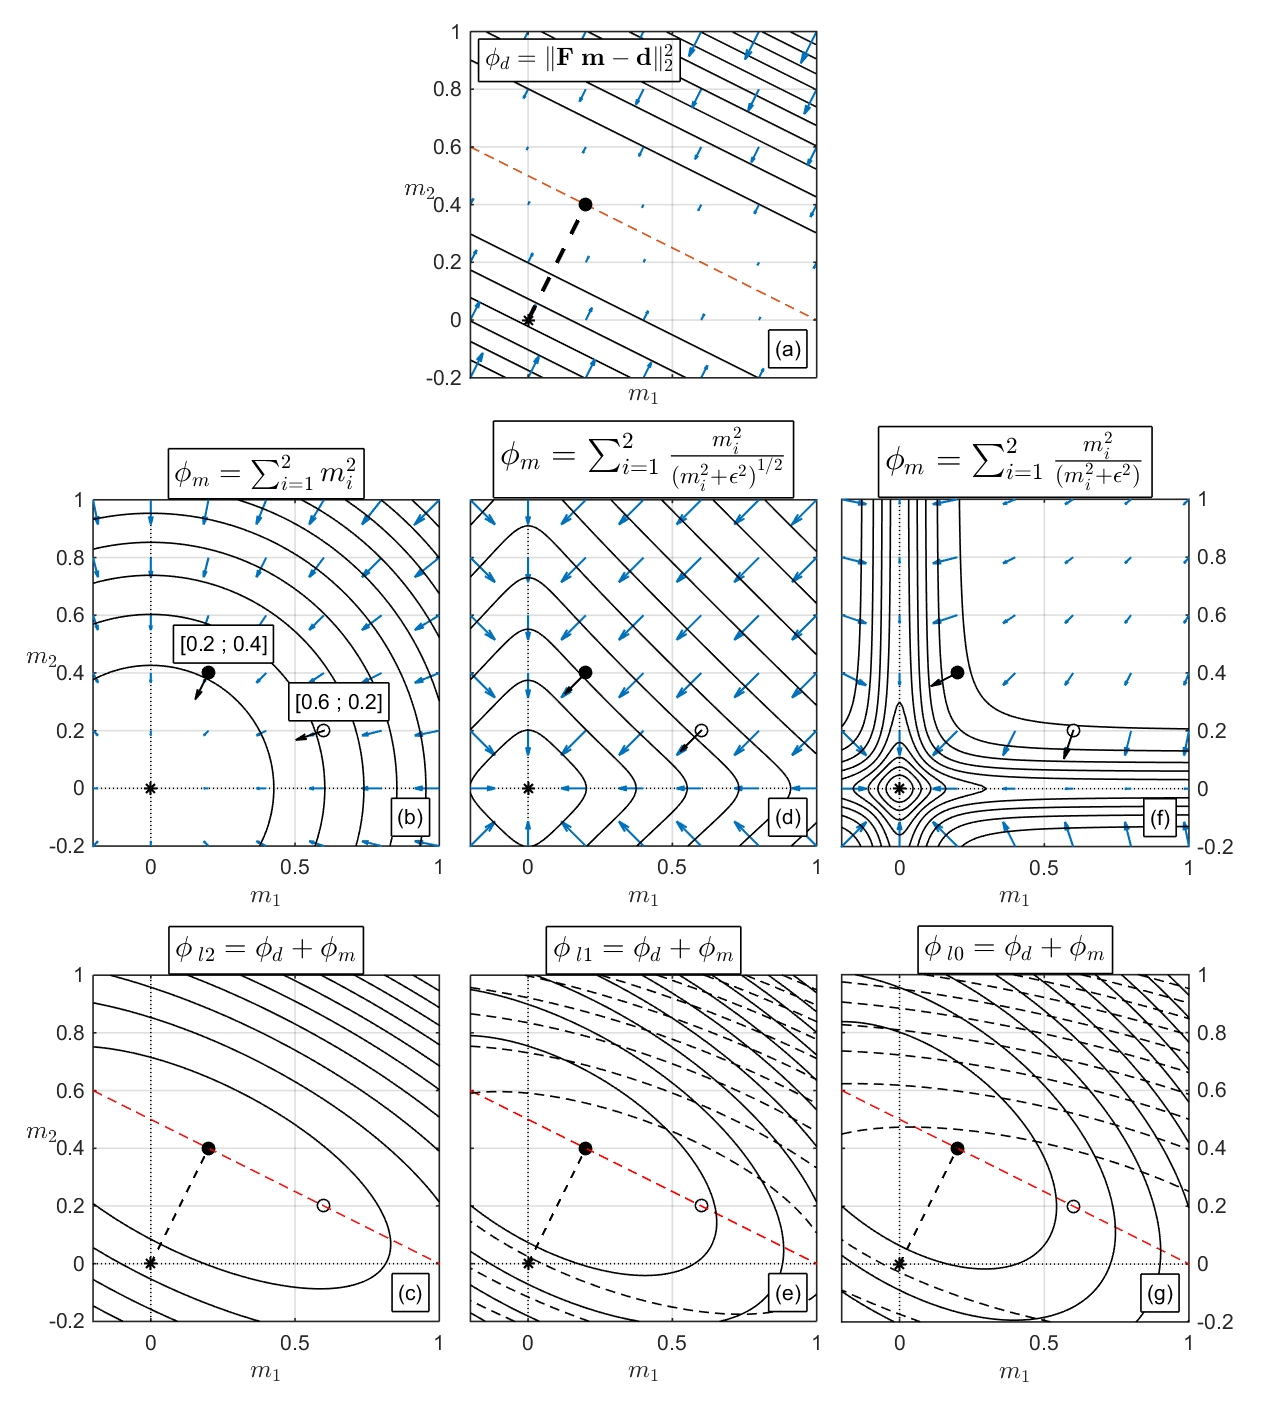
\includegraphics[scale=0.52]{IRLS_toy_l0l1l2}
\caption{Comparative contour maps for various objective functions over a range of model values $[ m_1 ;\;m_2 ]$. (a) The mininum of the misfit function $\phi_d$ forms a line spanned by $\mathcal{N} (\mathbf{F})$ (red dash). The $least-norm$ solution is marked as a solid dot. (Middle) Regularization functions and gradient directions (blue arrows) for approximated $l_p$-norm measures of the model for (b) $p=2$, (d) $p=1$ and (f) $p=0$.
The gradient directions are shown for two different starting models  (black arrows). 
(bottom) Contour maps of the initial objective functions $\phi(m) = \phi_d + \phi_m$ for the same two starting models: $\mathbf{m}^{(0)}_1$ (solid) and $\mathbf{m}^{(0)}_2$ (dash). (c) In the $l_2$-norm case , the function has a global minimum regardless of the starting model, while for non-linear functions for (e) $p=1$ and (g) $p=0$, the objective function changes with respect to the starting model.}
\label{fig:IRLS_toy}
\end{figure}

\begin{figure}[h!]
\centering
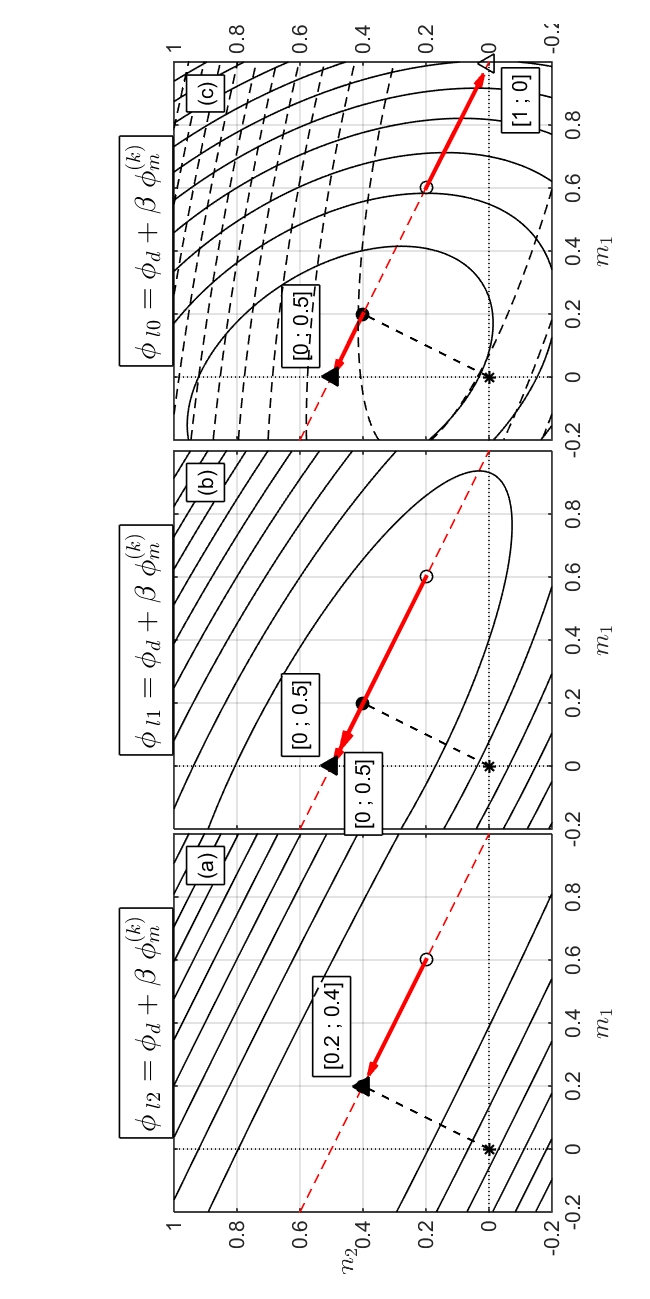
\includegraphics[scale=0.58,angle=270]{IRLS_toy_Result}
\caption{Contour maps for various objective functions after convergence of the IRLS algorithm. (a) Final model obtained with the $l_2$-norm penalty on the model for two starting models at $\mathbf{m}_1^{(0)}=[0.2;0.4]$ and $\mathbf{m}_2^{(0)}=[0.6;0.2]$ for a fixed trade-off parameter ($\beta = 1e-4$). In both cases, the solution converges to the global minimum, which is also the $least-norm$ solution at  $\mathbf{m_{ln}}=[0.2;0.4]$. 
(b) Solution with the $l_1$-norm penalty for the same starting models and trade-off parameter, converging to a global minimum at $\mathbf{m}^*=[0;0.5]$. This solution is sparse and can reproduce the data.
(c) The same experiment is repeated for the $l_0$-norm penalty, converging to two different solutions depending on the relative magnitude of the starting model parameters. Both solutions are sparse and honor the data. }
\label{fig:IRLS_toy_result}
\end{figure}

It is also important to note that the model norm regularization can be shifted away from the origin if we were to minimize:
\begin{equation}
\phi_m = \| \mathbf{m - m^{ref}} \|_2^2 \,.
\end{equation}
In this case, the minimum gradient of the objective function would occur at $\mathbf{m^{ref}}$. 
We would therefore look for a solution that both minimizes the data residual, while also approximating the expected model value. For simplicity, I consider the case where the reference model is at origin.

\section{$Lp$-norm and iterative re-weighted least squares} 
I have so far only considered the Euclidean norm of the model parameters,  penalizing the square of model values. 
Likewise, \cite{LiOldenburg1996} include an $l_2$-norm penalty on the model gradients, yielding smooth models.
In some cases, the solution may be expected to be sparse and blocky, either in terms of model parameters or spatial gradients. 
There have been several studies dedicated to the use of non-$l_2$ measures to recover models with sharp edges.
Most methods proposed in the literature made us of the globally convex $l_1$-norm, with proven convergence to a global minimizer \cite[]{FarquharsonOldenburg98, SunLi14, Daubechies10}.
Others have proposed approximations to the non-convex $l_0$-norm, methods such as the $compact$ regularization of \cite{ LastKubik83} and the $minimum\;support$ functional of \cite{Portniaguine1999}, to name a few.
My goal is to further generalize the proposed methods in order to explore a wide range of solutions for any combinations of $l_p$-norm penalty applied on the model and model gradients independently.

I begin with a generalized expression for the model objective function, such that \eqref{eq:obj_func} becomes:
\begin{equation} \label{eq:lpnorm}
\phi_m = \sum_{i=1}^{nc} \rho ( x_i ) \; ,
\end{equation}
where $\rho$ is some norm measure of a model function $\mathbf{x}(m)$ commonly chosen to be the model itself or some measure of spatial gradients. 
The general $l_p$-norm measure can be written as
\begin{equation} \label{eq:lpnorm}
\phi_m = \sum_{i=1}^{nc} {|x_i|}^p \;,
\end{equation}
where for $p=2$, I recover the standard regularized inversion presented in \eqref{eq:obj_func}.
Several approximations to the $l_p$-norm have been proposed, such as the Ekblom norm \cite[]{Ekblom73}: 
\begin{equation} \label{eq:Ekblom}
\phi_m =  \sum_{i=1}^{nc} {(x_i^2 + \epsilon^2)}^{p/2} \;,
\end{equation}
where a small number $\epsilon$ is added to guarantee that the function is continuous and differentiable as $\mathbf{x} \rightarrow 0$. 
Figure~\ref{fig:Lp_r_dphidm}(a) presents various norms for a fix threshold values ($\epsilon=1e-2$).
 The derivative of \eqref{eq:Ekblom} is given by:
\begin{equation} \label{eq:dphidm}
\begin{split}
\frac{\partial \phi_m}{\partial m} &= \sum_{i=1}^{nc} \rho'(x_i)  \frac{\partial x_i}{\partial m} \\
 &= p \;\frac{x_i}{{{(x_i}^{2} + \epsilon^2 )}^{1-p/2}}  \;  \frac{\partial x_i}{\partial m} \;.
\end{split}
\end{equation}
Expression \eqref{eq:dphidm} is clearly non-linear with respect to the model function $x_i$. 
As first introduced by \cite{Lawson61}, the norm can be linearized by the \emph{Iteratively Re-weighted Least-Squares} (IRLS) method such that:
 \begin{equation} \label{eq:IRLS_phi}
\phi_m^{(k)} =  \frac{1}{2}\sum_{i=1}^{nc} r_i \; x_i^2
\end{equation}
\begin{equation}\label{eq:IRLS_dphidm}
	\frac{\partial \phi_m^{(k)}}{\partial m}  =   r_i \; x_i \frac{\partial x_i}{\partial m} \;,
\end{equation}
where we added the superscript $\square^{(k)}$ to denote the IRLS iterations. The weights $r(x)$ are computed from model values obtained at a previous iteration such that:
\begin{equation}\label{eq:R_w}
	{r}_i  ={\Big( {({x_i}^{(k-1)})}^{2} + \epsilon^2 \Big)}^{p/2 - 1} \;,
\end{equation}
where ${r}(x) \in \mathbb{R}^{nc}$.

The goal of the IRLS method  is to approximate the $l_p$-norm by solving a series of locally convex least-squares problems.
The general objective function to be minimized takes the form:
\begin{equation}\label{eq:Lp_phi}
\begin{split}
\phi(m) &= \phi_d + \beta \phi_m^{(k)} \\
 &= \|\mathbf{ Fm - d }\|_2^{2} + \beta  \|\mathbf{ R\;x}(m) \|_2^{2} \;,
 \end{split}
\end{equation}
where the diagonal matrix $\mathbf{R} \in \mathbb{R}^{nc \times nc}$ holds the IRLS weights such that:
\begin{equation}
{R}_{ii} =  {{r}_i }^{1/2} \;.
\end{equation}
At each $k^{th}$ iteration, we seek a minimum along the gradient of the the objective function.
Replacing the regularization function from equation \ref{eq:dphi_dm} we get:
\begin{equation}\label{eq:dphi_dm_lp}
\begin{split}
 \mathbf{F^TF}\mathbf{m} + \beta\;\mathbf{g}(x) = \mathbf{F^T \; d} \\
\mathbf{g}(x) = \mathbf{R^TR\;x}(m) \frac{\partial \mathbf{x}(m)}{\partial m}\, ,
 \end{split}
\end{equation}
where I explicitly define the gradient of the approximated $l_p$-norm regularization function $\mathbf{g}(x)$.
I voluntarily neglect the constant of differentiation $p$ from equation \eqref{eq:IRLS_dphidm} for two reasons.
First, note that in the special case where $p=0$, the regularization function would vanish and reduce \ref{eq:dphi_dm_lp} to a simple least-squares problem.
Secondly, for any $p\ne0$, the constant would simply get absorbed by the trade-off parameter $\beta$.
Other parameters will be introduced in the following section to handle scaling issues arising from mixed-norm regularization functions.

Figure~\ref{fig:Lp_r_dphidm}(b) and (c) presents the IRLS weights $\mathbf{r}(x)$ and gradient functions $\mathbf{g}(x)$ for a range of $p$-value.
For $p=2$ and $\mathbf{x}(m) = \mathbf{m}$, we obtain the smooth regularization function presented in Figure~\ref{fig:IRLS_toy}(a).
It is important to note that for a small $l_p$-norm (i.e $p < 1$), the IRLS weights and gradients rapidly increase as $x_i \rightarrow \epsilon$.
The behavior of the regularization function around the threshold parameter $\epsilon$ is important for reasons that will be addressed in Section~\ref{eps_algo}.  

\begin{figure}[h!]
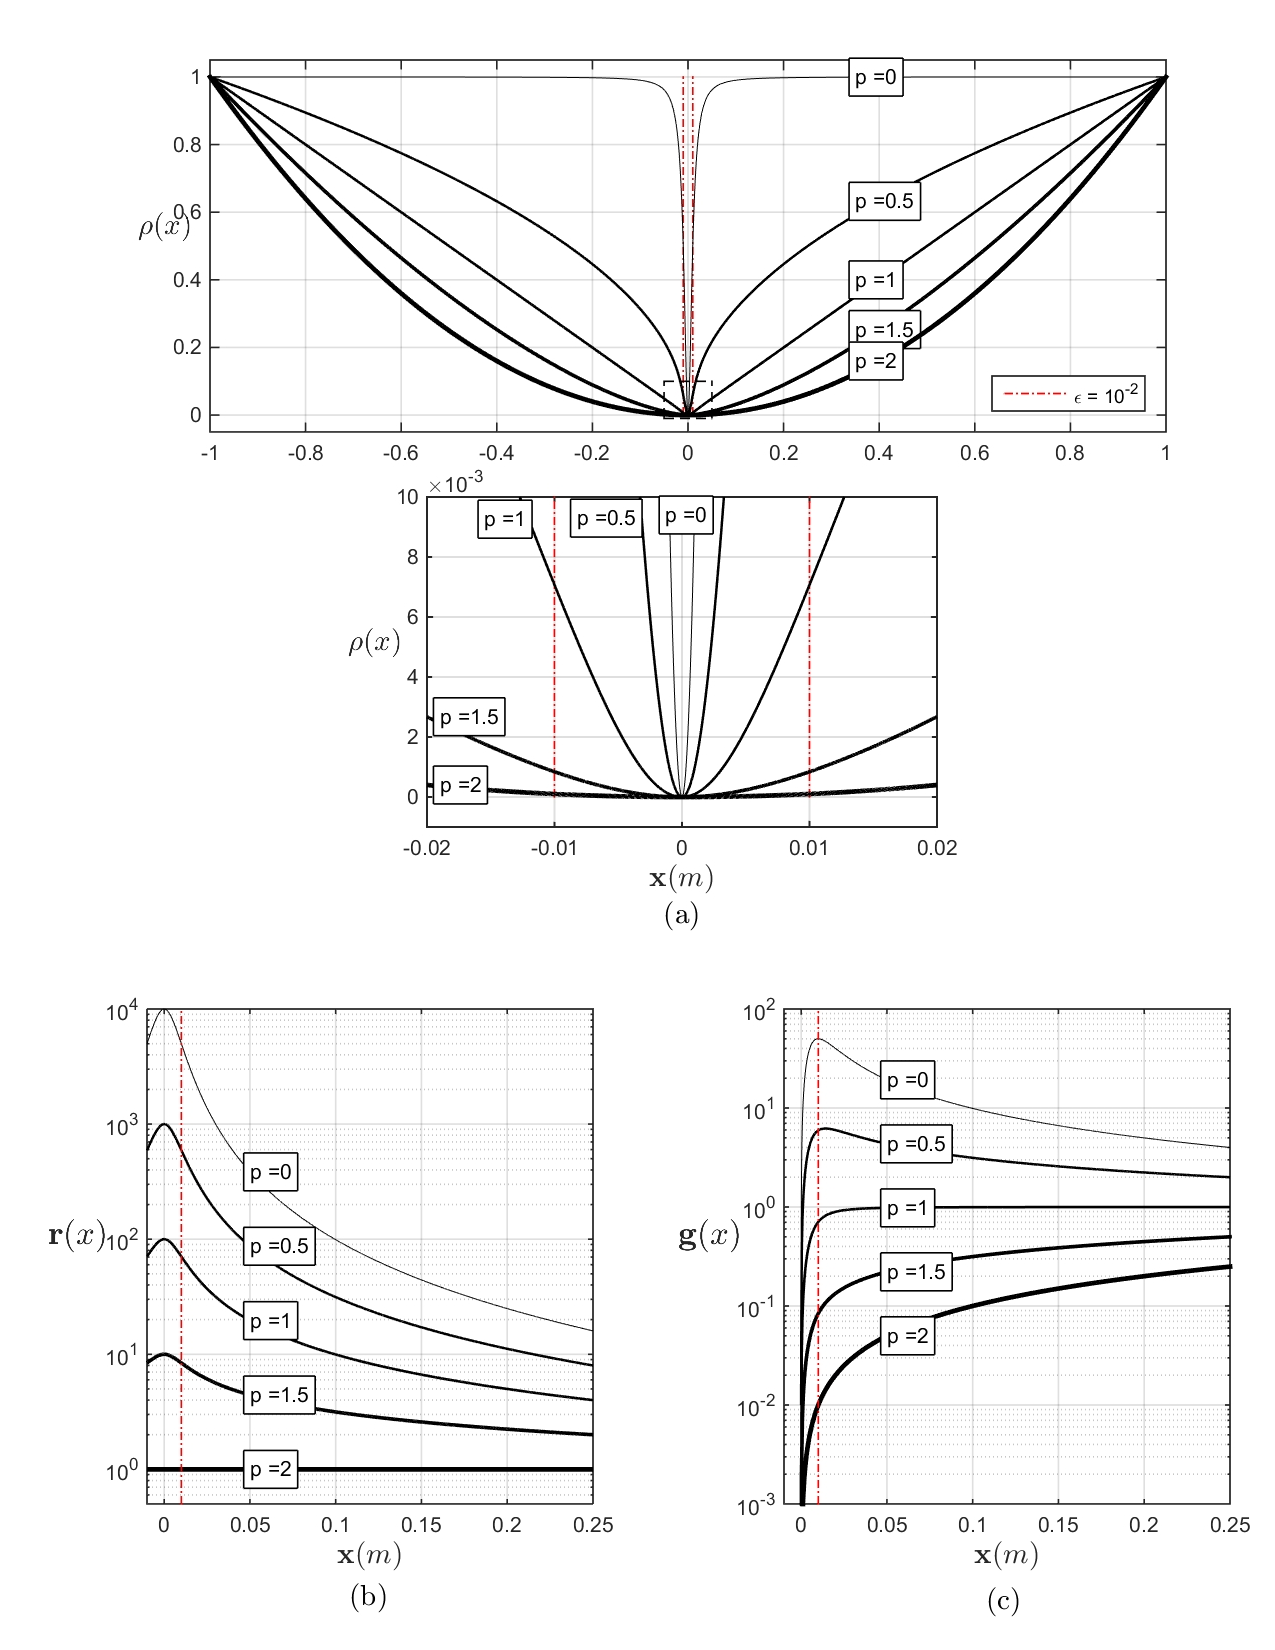
\includegraphics[scale=0.53]{Lp_r_dphidm}
\centering
\caption{(a) Penalty function $\rho(x)$ for different approximate $l_p$-norm measures, and enlarged view near the region of influence of $\epsilon$, making the $l_p$-norm continuous at the origin. (b) IRLS weights $\mathbf{r}(x)$ as a function of model function $\mathbf{x}(m)$ and $p$-values and for a fix threshold parameter ($\epsilon =1e-2$). (c)  Gradients $\mathbf{g}(x)$ of the model penalty function for various $p$-values. Note that the gradients are on a logarithmic scale due to the rapid increase as ${x}_i \rightarrow \epsilon$ for $p < 1$.}
\label{fig:Lp_r_dphidm}
\end{figure}

I illustrate the various $l_p$-norms on the same 2-variable inverse problem presented in Section~\ref{LN_and_RLS}.
Figure~\ref{fig:IRLS_toy}(d) and (e) show the regularization and the objective function for $p=1$, over a range of model parameters.
I point out that, compared to the globally convex $l_2$-norm, the shape of the objective function now depends on the starting model $\mathbf{m_1}^{(0)}$ and $\mathbf{m_2}^{(0)}$.

For $p = 0$, I recover the \textit{compact} regularization function put forward by \cite{ LastKubik83}, which has been borrowed by many researchers in geophysics \cite{BarbosaSilva94, Ajo-Franklin07, Stocco09}.
Figure~\ref{fig:IRLS_toy}(f) and (g) presents the approximated $l_0$-norm and corresponding objective function over the same range of model parameters. 
Similarly, the minimum of the objective function depends on the initial model $\mathbf{m}^{(0)}$ used to construct the regularization.

Although difficult to prove analytically, experiments have shown that the $l_0$-norm can yield a sparser solution than the convex $l_1$-norm \cite[]{Chartrand07}. 
I use the same 2-variable example to illustrate this idea.
For simplicity, I impose a fix threshold parameter ($\epsilon = 1e-8$) and a fix trade-off parameter ($\beta=1e-4$).
%\textemdash two small values found empirically to approximate the norm well while minimizing the data misfit. 
Here, I am only interested in the final solution depending on the choice of $l_p$-norm, and as a function of starting model $\mathbf{m}^{(0)}$. 
In the next section, I will provide strategies to efficiently determine those parameters.

In the first experiment, I choose the starting model $\mathbf{m_1}^{(0)}$ to be the least-norm solution at $\mathbf{m_{ln}}$= [0.2;0.4], marked as a solid dot (Fig.~\ref{fig:IRLS_toy_result}). 
In both cases the $l_1$-norm and $l_0$-norm converge to the same optimal solution at $\mathbf{m^{*}}$= [0.0;0.5].
The model $\mathbf{m^{*}}$ is interesting as it is sparse with a single non-zero parameter, while also having the smallest norm possible.

In the second experiment, the initial model is also chosen to satisfy the target data misfit, but this time with a relatively smaller value on the second variable such that $\mathbf{m_2}^{(0)}$= [0.6;0.2], marked as a white dot. 
Because both the $l_1$-norm and $l_0$-norm penalize small model parameters, the regularization forces the solution to be sparse along $\mathcal{N} (\mathbf{F})$. 
Note the clear difference between the globally convex $l_1$-norm, converging back to $\mathbf{m^{*}}$, compared to the non-convex $l_0$-norm, reaching the $m_1$-axis at $\mathbf{m}^{(k)}$= [1;0]. 
The $l_0$-norm has therefore two possible solutions that do not depend on the overall magnitude of $\mathbf{m}^{(0)}$, but rather on the \emph{relative} magnitude of its components $[m_1\;;\;m_2]$. 
The $l_0$-norm acts as a binary selector, influenced by the largest elements of a starting model.

The choice of specific norm should therefore reflect the expected character of the solution, and the chosen algorithm should allow access to the full range of norms for $0\leq p \leq 2$.
While it is simple to solve \eqref{eq:Lp_phi} for a 2-variable problem, finding a solution to large systems for non-convex norms ($p < 1$) has proven to be difficult and remains a field of active research. 
%\cite[]{ PortniaguineZhdanov02, Ajo-Franklin07, SunLi14, Stocco09, BarbosaSilva94}. 
The following sections review potential complications for the non-convex cases, and review strategies to efficiently solve the IRLS method.

%%%%%%%%%%%%%%%%%%%%%%%%%%%%%%%
\section{IRLS solver}\label{Solve_IRLS}
The IRLS method presented in \ref{eq:Lp_phi} is an iterative process, which depends on two key parameters: the trade-off parameter $\beta$ and the threshold parameter $\epsilon$.
In this section, I explore four strategies for the implementation of the IRLS.

\subsection{Basic IRLS algorithm}
As illustrated with the previous 2-variable problem, the choice of a starting model $\mathbf{m}^{(0)}$ is especially important for non-convex norms $p < 1$.
According to \cite{Chartrand07}, it may be possible to compute a global minimizer from non-convex functions, as long as the initial model is close enough to the global optimum.
Most methods proposed in the literature seem to agree on the $l_2$-norm solution as a valid candidate \cite[]{ PortniaguineZhdanov02, Ajo-Franklin07, SunLi14}.
Current inversion strategies already rely on the assumption that a smooth model is a good approximation of the true solution.
Applying a sparse $l_p$-norm can then segregate the most important model parameters, which in turn can reduce the complexity of the solution. 
This is mostly interesting if the true solution is known to behave like a delta function. 

The basic IRLS algorithm becomes a two step process, as summarized in Table~\ref{tbl:IRLS_v1}.
During Phase-I, the algorithm finds a smooth solution with the $l_2$-norm regularization.
The trade-off parameter $\beta$ is monotonically reduced until the model can predict the data near the target misfit $\phi_d^*$.
The final $l_2$-norm solution provides a starting model $\mathbf{m}^{(0)}$ for the calculation of a weighting matrix $\mathbf{R}$.

In Phase-II of the IRLS method, model updates are computed iteratively by minimizing \ref{eq:Lp_phi}.
This process is repeated until the algorithm converges to a stable solution.
I define a $convergence$ criteria as:
\begin{equation}\label{Convergence}
\begin{split}
\delta \phi_m^{(k)} & = \frac{|\phi_m^{(k)} - \phi_m^{(k-1)}|}{\phi_m^{(k)}} \times 100\% \;,
\end{split} 
\end{equation} 
where the change in model norm falls below some pre-defined threshold, chosen to be 2\% in all my experiments.
In the simplest form of the algorithm, the threshold $\epsilon$ and trade-off parameter $\beta$ remain constant throughout Phase-II.
For now, I will follow the general consensus that $\epsilon$ has to be small, or near machine error ($\epsilon_p = \epsilon_q = 1e-8$) \cite[]{LastKubik83,Ajo-Franklin07, Stocco09}.
I will revisit this number in Section~\ref{eps_algo}.
In the method proposed by \cite[]{Ajo-Franklin07}, a trade-off parameter $\beta^*$ is chosen so that the initial IRLS solution predicts the data near the target misfit $\phi_d^*$. 
This $\beta^*$ then remains constant throughout the iterative process.

\begin{table}[h!]
\centering
\caption{IRLS Solver 1: Fix parameters}
\label{tbl:IRLS_v1}
\renewcommand{\arraystretch}{1.5}
\begin{tabular}{|c|}\hline
\textbf{Phase I - $L_2$-norm iterations:  $\left\{ \mathbf{m}^{(0)} \mid \phi_d \simeq \phi_d^* \right \}$}\\
Adjust $\beta$ \\
$min\; \phi(m)  \rightarrow \mathbf{m}^{(0)}$ \\ \hline
Search:   $\left\{  \beta^* \mid \phi_d^{(k)} \simeq \phi_d^* \right \}$\\ \hline
\textbf{Phase II - $L_p$-norm iterations: $\left\{  \mathbf{m}^{(k)} \mid \delta \phi_m^{(k)} < 1\%  \right \}$ }\\
Fix \{$\beta^*, \epsilon_p,\epsilon_q$\}\\
Update $r_i^{(k)}$\\
$min\; \phi^{(k)}  \rightarrow \mathbf{m}^{(k)}$\\ \hline
\end{tabular}
\end{table}

\subsection{1-D synthetic example}
I demonstrate this simple IRLS implementation on a synthetic 1D problem similar to the problem used by \cite{LiOldenburg1996}.
The model consists of a rectangular pulse and a Gaussian function on the interval [0 1] and discretized with 200 uniform intervals. Data are generated from the equation:
\begin{equation} \label{eq:9}
  d_j = \int_0^1 f_j(x) m(x) \; dx, \:\: j = 0, ..., N\;,
\end{equation}
where the kernel functions relating the model and the data are defined as:
\begin{equation} \label{eq:kernel_1D}
  f_j(z) = e^{-j\:x }\cdot cos(2 \pi j x) \;,
\end{equation}
where $x$ defines the distance along the $x$-axis. 

The model and kernel functions for $j \in [1 , 30]$ are shown in Figure \ref{fig:1D_model}. 
Two percent random noise is added to the data in order to simulate a true geophysical experiment. 
The data are weighted accordingly such that:
\begin{equation} \label{eq:Weighted_misifit}
	\phi_d = \|\mathbf{W_d \;( F\;m - d)}\|_2^{2}\;,
\end{equation}
where the diagonal matrix $\mathbf{W_d}$ holds the estimated uncertainties associated with each datum. 
Since the noise is assumed to be Gaussian and uncorrelated, the misfit function follows a chi-squared distribution with expected value of $N$, hence the target misfit.

\begin{figure}[h!]
\centering
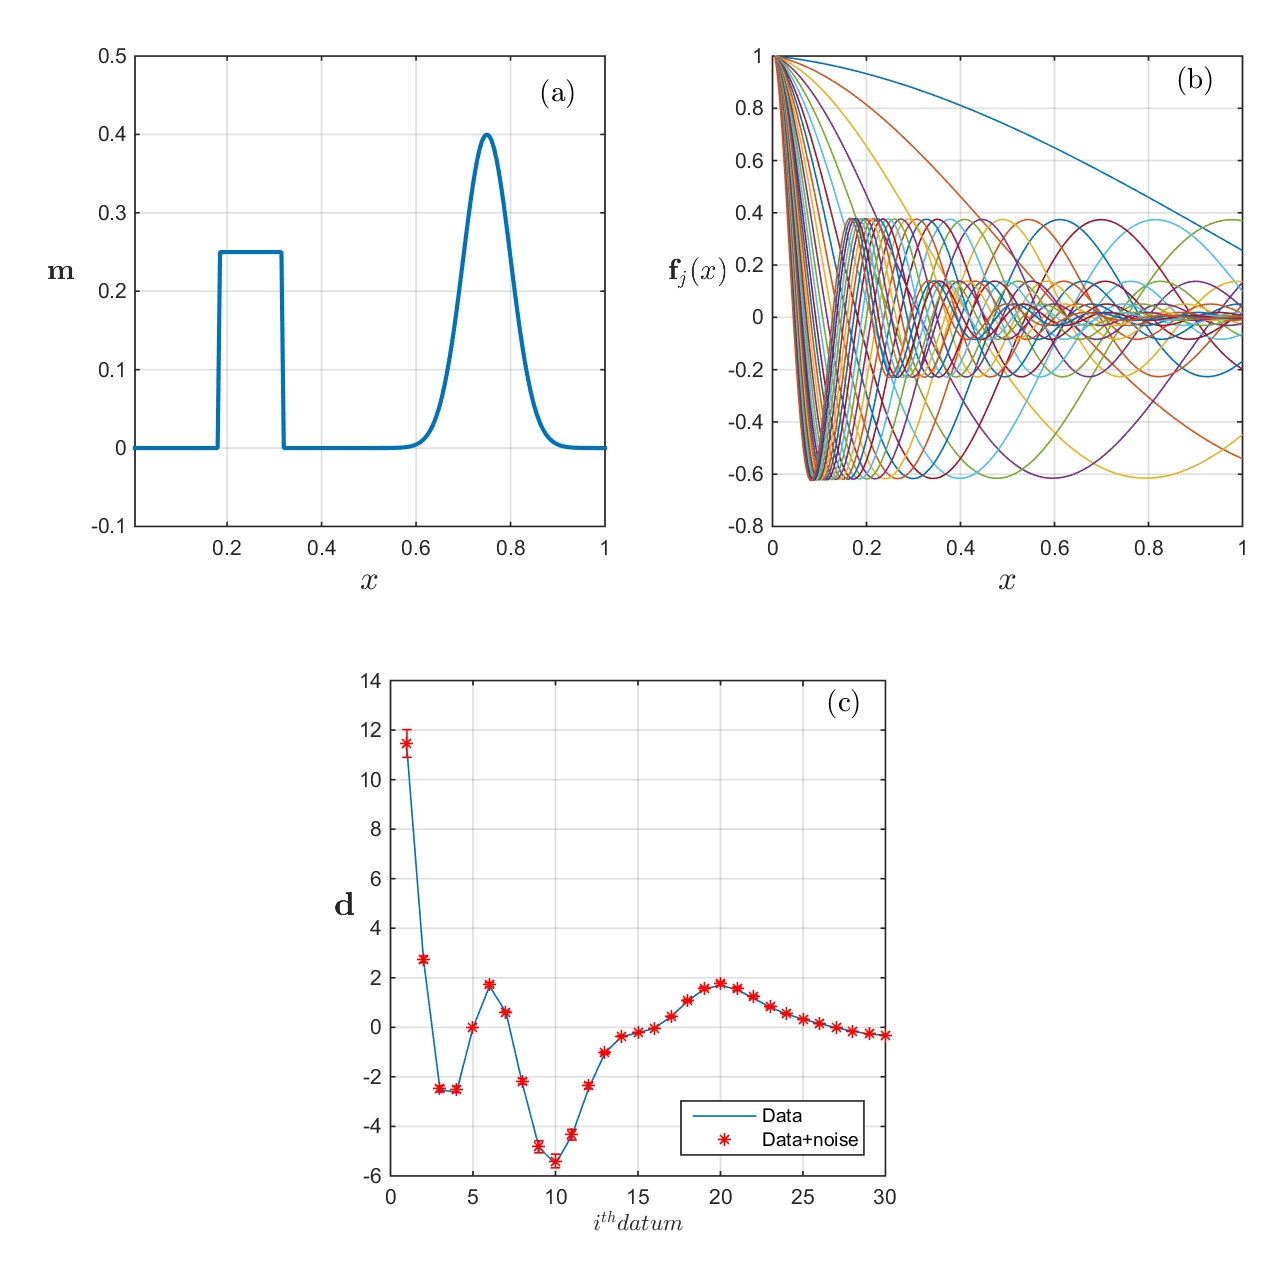
\includegraphics[scale=0.55]{1D_Kernel_data}
\caption{(a) Synthetic 1D model made up of a rectangular pulse and a Gaussian function. (b) Kernel functions consisting of exponentially decaying cosin functions of the form $ f_j(x) = e^{-j\:x }\cdot cos(2 \pi j x)$. (c) Data generated from $\mathbf{d =F \; m}$ , with $5\%$ random  Gaussian noise added. }
\label{fig:1D_model}
\end{figure}

I here generalize the objective function presented in Chapter~\ref{ch:Chap3_Inverse} to allow for multiple $l_p$-norm regularization functions such that:
\begin{equation} \label{eq:Lp_phi_int}
\phi(m) =  \phi_d + \beta \Big [ \int_0^1 w_s \; {\left|m - m^{ref}\right|^p} \; dl + \int_0^1 w_x\; {\left|\frac{\partial m}{\partial x}\right|^{q}} \;dl \Big ]\;.
\end{equation}
The only difference with the regularization function used in \ref{eq:Phi_int} is in the norms applied on the model and model gradients ${|\cdot|}^p$ and ${|\cdot|}^q$, where $p$ and $q$ can take any value on the interval $[0, 2]$.
Since we are dealing with a 1-D problem, model gradients are only computed along the $x$-axis.
I also apply a depth weighting function to counter the decay of the kernel functions such that:
\begin{equation}\label{DepthWeight}
\begin{split}
w_s = \alpha_s\; e^{jx}\\
w_x = \alpha_x\; e^{jx}\;.
\end{split}
\end{equation}
Combining the IRLS approximation in \eqref{eq:Lp_phi} and the discrete objective function presented in \ref{eq:Phi_disc}, the linear 1-D equation \ref{eq:Lp_phi_int} becomes:
 \begin{equation} \label{eq:Lp_phi_1D}
\phi(m) =  \|\mathbf{W_\text{d} \;( F\;m - d)}\|_2^{2} + \beta \Big [ {\| \mathbf{W}_s \; \mathbf{R}_s\; ( \mathbf{m - m^{ref}})\|}^2_2  + {\|   \mathbf{W}_x  \; \mathbf{R}_x\; \mathbf{G}_x \; \mathbf{m}\|}^2_2  \Big ]\;,
\end{equation}
where the diagonal matrices $\mathbf{W}_s,\mathbf{W}_x$ are the cell weights, and $\mathbf{G}_x$ is the spatial gradient operator presented in Chapter~\ref{ch:Chap3_Inverse}.
The IRLS weights $\mathbf{R}_s$ and $\mathbf{R}_x$ are defined as:
\begin{equation}\label{eq:Rs_Rx}
\begin{split}
	{R}_{s_{ii}}  &= {\Big[ {({m_i}^{(k-1)})}^{2} + \epsilon_p^2 \Big]}^{(p/2 - 1)/2} \\
	{R}_{x_{ii}}  &= {\Big[ {\left ({\frac{\partial m_i^{(k-1)} }{\partial x}}\right)}^{2} + \epsilon_q^2 \Big]}^{(q/2 - 1)/2}  \;,
\end{split}
\end{equation}
where $\epsilon_p, \epsilon_q$ are the stabilizing parameters for the sparsity constraint applied on the model and model gradient respectively.

As explained in Section \ref{Iterative solver}, the minimum norm solution is found where $\frac{\partial \phi(m)}{\partial m} = 0$.
Taking the partial derivatives of \ref{eq:Lp_phi_1D} with respect to the model parameters and setting the reference model to zero yields:
\begin{equation}\label{eq:dphi_dm_inv}
\Big ( \mathbf{F^TW_\text{d}^TW_\text{d}F} + \beta \big [ \mathbf{R}_s^{\mathbf{T}}\; \mathbf{W}_s^{\mathbf{T}} \mathbf{ W}_s \;\mathbf{ R}_s + \mathbf{G}_x^{\mathbf{T}} \;\mathbf{R}_x^{\mathbf{T}}\; \mathbf{W}_x^{\mathbf{T}}\mathbf{ W}_x \;\mathbf{R}_x \; \mathbf{G}_x \; \big]\Big ) 
\mathbf{m = F^TW_\text{d}^TW_\text{d}d} \;.
\end{equation}
This linear system can be expressed as an overdetermined problem of the form:
\begin{equation}\label{eq:lsqr_IRLS_dphi_dm}
 \begin{bmatrix}
\mathbf{W_\text{d}} \;\mathbf{F} \\
\sqrt{\beta} \mathbf{W}_s \;\mathbf{R}_s\\
\sqrt{\beta} \mathbf{W}_x \;\mathbf{R}_x \;\mathbf{G}_x \\
 \end{bmatrix} \mathbf{m} =
   \begin{bmatrix}
\mathbf{W_\text{d}} \; \mathbf{d}\\
0 \\
0
 \end{bmatrix} \;.
 \end{equation}
Solving the least-squares problem \ref{eq:lsqr_IRLS_dphi_dm} yields a model update at the $k^{th}$ iteration of the IRLS method.
In this case, the left-hand side of \ref{eq:dphi_dm_inv} is linear with respect to $\mathbf{m}^{(k)}$ and it forms a symmetric positive definite matrix, which can be solved efficiently by the Conjugate Gradient descent method.

For the initial phase of the IRLS method, a solution is found with the globally convex $l_2$-norm regularization, in which case $\mathbf{R}_s$ and $\mathbf{R}_x$ reduce to the identity matrix.
Figure \ref{fig:1D_IRLS_algo1}(a) presents the inverted result obtained with the $l_2$-norm, as well as the convergence curve after achieving the target data misfit $\phi_d^*$. 
As expected from an $l_2$-norm regularization, the solution is smooth and dispersed over the entire model domain.

\begin{figure}[p]
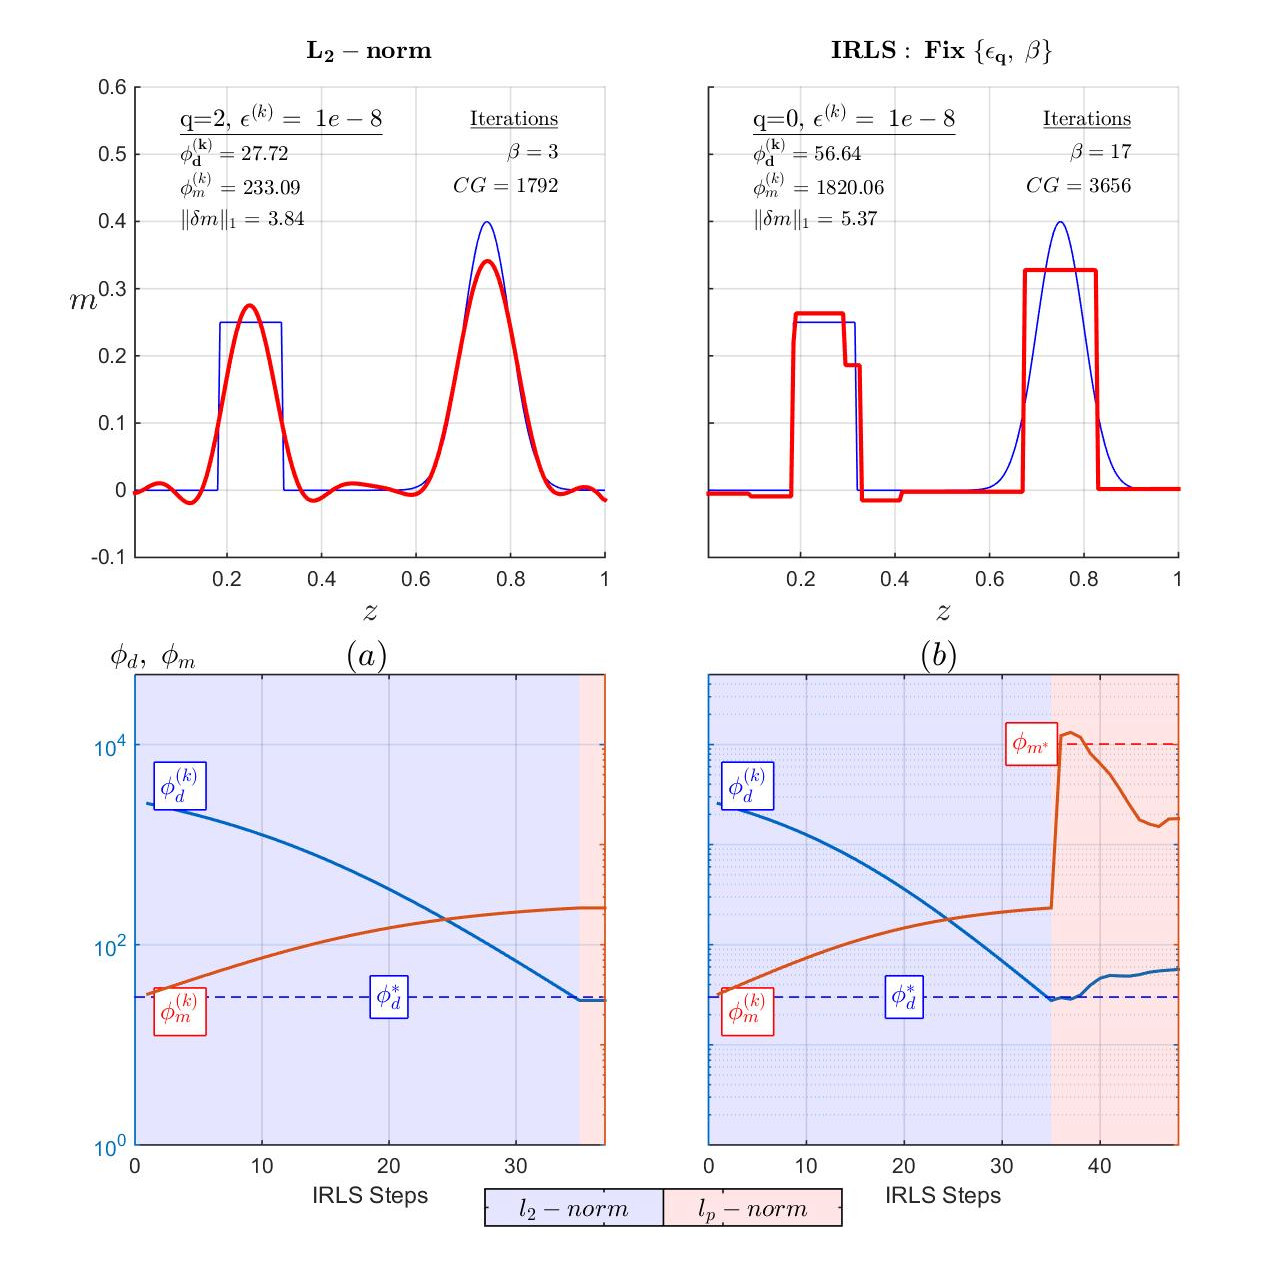
\includegraphics[scale=0.6]{1D_IRLS_algo1}
\caption{(a) Recovered models from the smooth $l_2$-norm regularization, and (bottom) measure of model misfit and model norm as a function of iterations. Both the rectangular pulse and Gaussian function are recovered at the right location along the $x$-axis, but the solution is smooth and dispersed over the entire model domain. (b) Solution obtained from the IRLS with spasity constraints on the model gradients ({q=0}), using the $l_2$-norm model (a) to initiate the IRLS steps. The algorithm uses a fixed threshold parameter ($\epsilon=1e-8$) and fixed trade-off parameter $\beta$. The final solution is blocky, as expected from the norm chosen, but fails to achieve the target data misfit. Clearly the influence of the regularization function has overtaken the minimization process.}
\label{fig:1D_IRLS_algo1}
\end{figure}

From there, the algorithm proceeds with a sequence of IRLS iterations with $l_0$-norm penalty on the model gradient ($\alpha_s=0, q =0$).
The goal is to use the regularization to enforce a solution with sharp gradients and hopefully recover the rectangular pulse.
The IRLS weights are initiated with the smooth $l_2$-norm solution.
The initial $\beta^*$ is found by a search method where a solution to equation~\ref{eq:lsqr_IRLS_dphi_dm} is computed for multiple trials.
The iterative process is repeated until the inversion reaches the convergence criteria specified by equation~\ref{Convergence}, while keeping the trade-off parameter $\beta^*$ constant.

As shown in Figure~\ref{fig:1D_IRLS_algo1}(b), the updated solution with the $l_0$-norm penalty recovers a blocky model with sharp edges. 
It is important to note that the final data residual $\phi_d^{(k)}$ is much larger than the target misfit ($\phi_d^*=30$).
Clearly the influence of the regularization has overtaken the inversion process.
The algorithm likely converged to some local minimum, far from the global optimizer previously found with the smooth $l_2$-norm.
Since I know the true solution, I can measure the accuracy of the solution, or model error as:
\begin{equation}
\| \delta m \|_1 = \sum_{i = 1}^{nc} |m_i^{(k)} - m_i^*| \;,
\end{equation}
where $\mathbf{m}^{(k)}$ is the solution found at the $k^{th}$ iteration.
The final model error is larger than the one found with the smooth $l_2$-norm regularization, hence it is a poor estimate of the true solution.

This example clearly illustrates some of the challenges related to non-convex objective functions.
We have so far only formulated the basic algorithm behind the IRLS method, which has been used by many researchers in the past.
Important details regarding the stability and predictability of the algorithm will now be addressed.

\subsection{Regularization scaling}
Following Tikhonov's approach, a solution to the inverse problem is found by progressively reducing the influence of the regularization until reaching the target data misfit $\phi_d^*$. 
For strictly convex regularization functions, such as the $l_2$-norm, the influence of the regularization functions is scaled linearly by the trade-off  parameter $\beta$. 
For non-convex functions, in our case for $q = 0$, the iteration process involves non-linear transformations of the objective function, driven by the IRLS weights computed in \eqref{eq:R_w}. 
Those weights can change rapidly as $\epsilon \rightarrow 0$, which directly impacts the influence of the model norm in a non-linear fashion. 
As demonstrated in Figure~\ref{fig:1D_IRLS_algo1}(b), special care must be taken in order to obtain a solution that satisfies the data while also being sparse.

As a second strategy, I experiment with a brute-force approach where the optimal trade-off parameter $\beta$ is determined before each IRLS steps (Table~\ref{tbl:IRLS_v2}).
A solution to \ref{eq:dphi_dm_lp} is computed several times for a range of $\beta$-values until a suitable trade-off parameter is found.
Figure~\ref{fig:1D_IRLS_algo2}(a) presents the model and convergence curve following this strategy.
The solution is blocky, as expected from the $l_0$-norm on model gradients, while also honoring the data within $1\%$ of the target misfit.
This iterative process is very expensive however, as it requires multiple $\beta$ solves per IRLS iteration.
For large non-linear problems, this type of approach would be computationally prohibitive.

\begin{table}[h!]
\centering
\caption{IRLS Solver 2: $\beta$-search}
\label{tbl:IRLS_v2}
\renewcommand{\arraystretch}{1.5}
\begin{tabular}{|c|}\hline
\textbf{Phase I - $L_2$-norm iterations:  $\left\{ \mathbf{m}^{(0)}, \beta^{(0)} \mid \phi_d \simeq \phi_d^* \right \}$}\\
Adjust $\beta$ \\
$min\; \phi(m)  \rightarrow \mathbf{m}^{(0)}$ \\ \hline
\textbf{Phase II - $L_p$-norm iterations: $\left\{  \mathbf{m}^{(k)} \mid \delta \phi_m^{(k)} < 1\% \right \}$ }\\
Fix \{$\epsilon_p,\epsilon_q$\}\\
Update $r_i^{(k)}$\\
Search:   $\left\{  \beta^{(k)} \mid \phi_d^{(k)} \simeq \phi_d^* \right \}$\\
$min\; \phi^{(k)}  \rightarrow \mathbf{m}^{(k)}$\\ \hline
\end{tabular}
\end{table}

\begin{figure}[p]
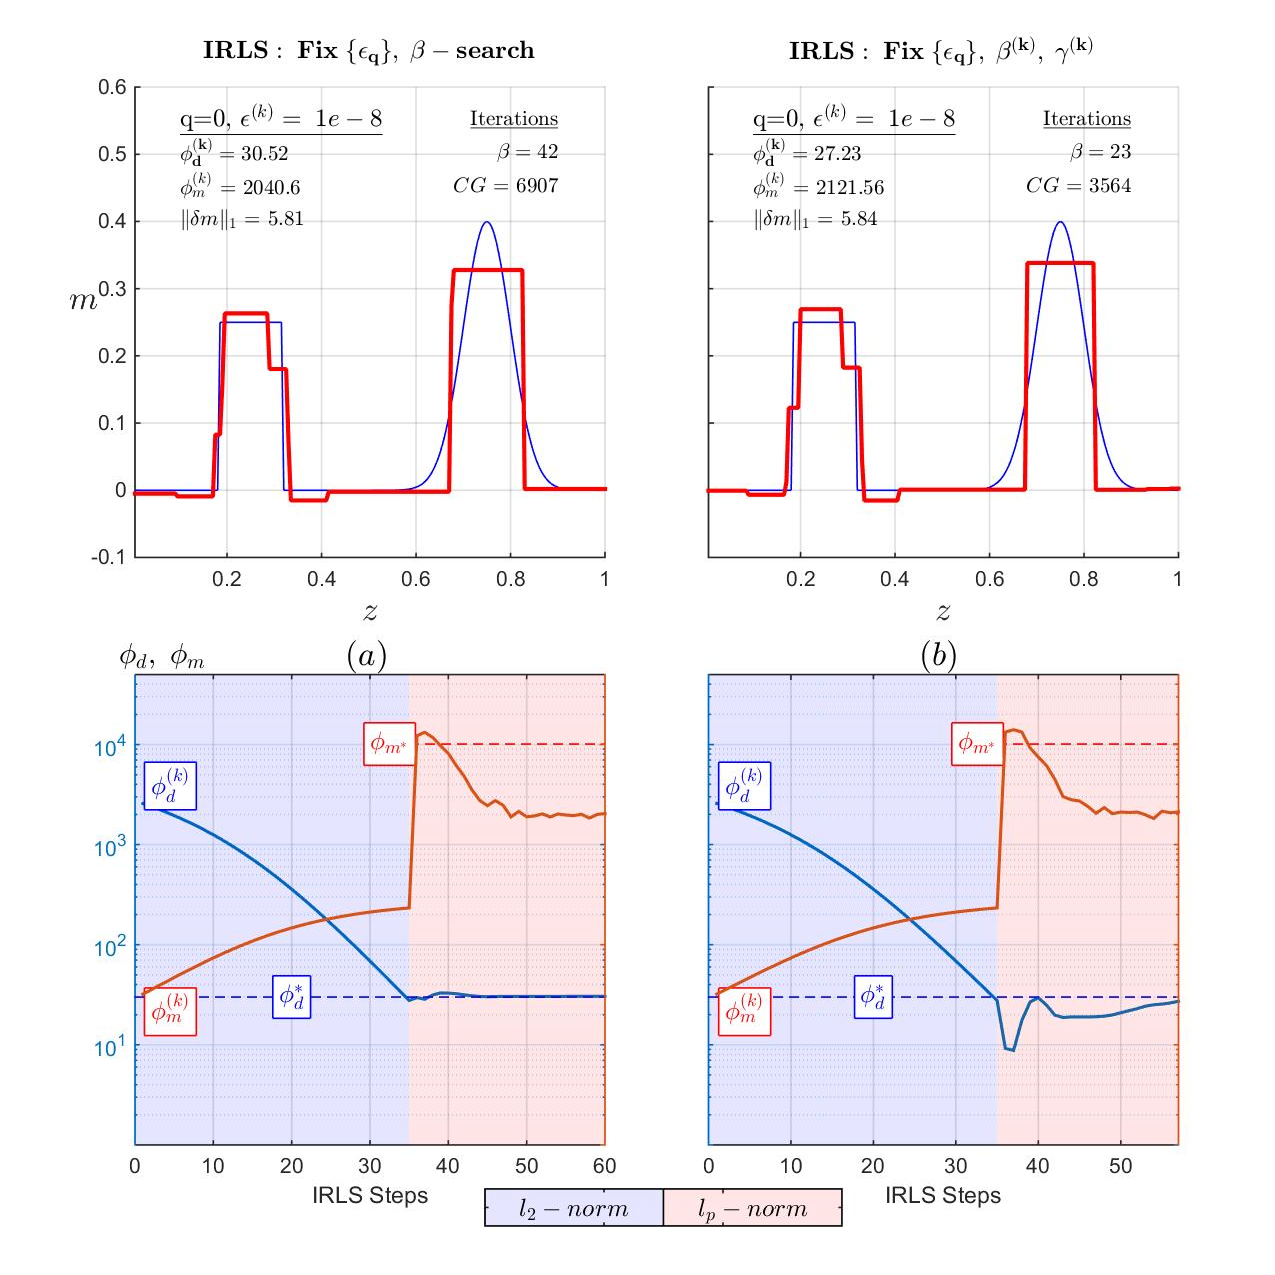
\includegraphics[scale=0.6]{1D_IRLS_algo2}
\caption{(Top) Recovered models from two different algorithms used to implement the IRLS method for $q=0$ and a fix threshold parameter ($\epsilon=1e-8$). (Bottom) Measure of model misfit and model norm as a function of iterations. (a) The first algorithm searches for an optimal trade-off parameter $\beta^{(k)}$ between each IRLS step, requiring a solution to multiple sub-inversions. (b) The second algorithm only adjusts $\beta^{(k)}$ once after each IRLS step. A new scaling parameter $\gamma^{(k)}$ is added to smooth the transition between the IRLS updates. The algorithm recovers a similar blocky model but is computationally cheaper, as indicated by the total number of beta iterations and CG solves.}
\label{fig:1D_IRLS_algo2}
\end{figure}

As a third strategy, I relax the requirement for the model to predict the data $exactly$ between each IRLS steps. 
The trade-off parameter is adjusted once after each IRLS step such that:
\begin{equation}
\beta^{(k+1)} = \beta^{(k)} * \frac{\phi_d^*}{\phi_d^{(k)}} \;.
\end{equation}
I have found experimentally however that this type of posterior update is not sufficient to guarantee a smooth convergence. 
The initial IRLS update can change the model substantially, moving away from the global $l_2$-norm solution. 
In order to preserve the relative importance between misfit and regularization functions while reducing the computational cost, I propose an iterative re-scaling of the model objective function such that:
\begin{equation}\label{eq:scaled_Lp_phi}
\begin{split}
\hat \phi_m^{(k)} = \gamma^{(k)} & \Big ( {\| \mathbf{W_\text{s} \; R_\text{s} \; m}\|}^2_2 +  {\|  \mathbf{ W_\text{x}\; R_\text{x} \; G_\text{x} \; m}\|}^2_2  \Big ) \\
 \gamma^{(k)}  &= \frac{\hat \phi_m^{(k-1)}}{  {\| \mathbf{W_\text{s} \; R_\text{s} \; m}^{(k-1)}\|}^2_2 + {\|  \mathbf{W_\text{x}\; R_\text{x} \; G_\text{x} \; m}^{(k-1)}\|}^2_2 }\;,
 \end{split}
\end{equation}
where $\phi_m^{(k)}$ is the scaled model objective function at some $k^{th}$ iteration, and $\gamma^{(k)}$ is a scalar computed at the beginning of each IRLS iterations. 
Effectively we are searching  for model parameters that are close to the present solution.
Since we are changing the $rule$ by which the size of the model is measured, we attempt to account for it. 
I point out that for constant $l_p$-norm regularizations, the scaling parameter $\gamma^{(k)}$ is equal to one.
Table~\ref{tbl:IRLS_v3} summarizes the proposed method.

\begin{table}[h!]
\centering
\caption{IRLS Solver 3: Scaled regularization}
\label{tbl:IRLS_v3}
\renewcommand{\arraystretch}{1.5}
\begin{tabular}{|c|}\hline
\textbf{Phase I: $L_2$-norm iterations  $\left\{ \mathbf{m}^{(0)}, \beta^{(0)} \mid \phi_d \simeq \phi_d^* \right \}$}\\
Adjust $\beta$ \\
$min\; \phi(m)  \rightarrow \mathbf{m}^{(0)}$ \\ \hline
\textbf{Phase II: $L_p$-norm iterations $\left\{  \mathbf{m}^{(k)} \mid \delta \phi_m^{(k)} < 1\%,\; \phi_d \simeq \phi_d^* \right \}$ }\\
Fix \{$\epsilon_p,\epsilon_q$\}\\
Update $r_i^{(k)}$\\
Scale $\hat \phi_m^{(k)}$ \\
$min\; \phi^{(k)}  \rightarrow \mathbf{m}^{(k)}$\\ 
$\beta^{(k+1)}=\beta^{(k)} *\frac{\phi_d^*}{\phi_d^{(k)}} $\\ \hline
\end{tabular}
\end{table}
As shown in Figure \ref{fig:1D_IRLS_algo2}(b), the re-scaling procedure greatly reduces the total number of CG solves. 
Even though nothing guarantees that non-convex norms will converge to a $global$ minimum, the re-scaling scheme proposed here forces local minima to be in the proximity of the $l_2$-norm solution.
In other words, the scaling parameter $\gamma^{(k)}$ helps preserve the character of all previous iterations, slowly converging to a new minimum, hopefully in the vicinity of the global $l_2$-norm solution.

\subsection{Threshold parameter $\epsilon$}\label{eps_algo}
I have so far delayed providing details regarding the choice of threshold parameter $\epsilon$, which has been the subject of disagreement among researchers \cite[]{LastKubik83, BarbosaSilva94, Ajo-Franklin07, Stocco09, SunLi14}.  
Little has been said in the literature on how to determine a specific value of $\epsilon$.

In the classic work of \cite{LastKubik83}, and many other research papers after, it has been suggested that the stabilizing parameter should be small ($\epsilon < 10^{-8}$), or near machine error in order to approximate the $l_p$-norm well. 
Other researchers, such as in \cite{Ajo-Franklin07} have observed severe instabilities with such a small value, and found experimentally that $\epsilon$ should be between $10^{-4}$ and $10^{-7}$.
This may be due to the large spread in weights along the diagonal of \textbf{R} impacting the conditioning of the linear system described in equation \eqref{eq:dphi_dm}. A large condition number can adversely affect the convergence rate of gradient descent solvers.

As an alternative to the regularization function used by \cite{ LastKubik83}, \cite{Gorodnitsky97} apply the IRLS weights directly to the sensitivity matrix . The general objective function to be minimized takes the form:
\begin{equation}\label{eq:Lp_Jweighted}
 \phi = \|\mathbf{ \hat F \hat m - d }\|_2^{2} + \beta \|\mathbf{ \hat x}(m) \|_2^{2} \;,
\end{equation}
where the weighted forward model operator is written as:
\begin{equation}\label{eq:m_weighted}
 \mathbf{ \hat F = F}\;diag[\mathbf{m}^{(k-1)}]\;.
\end{equation}
The same technique was later revised by \cite{Portniaguine1999, PortniaguineZhdanov02} and coined Minimum Support (MS) functional.
The method was extended to penalties on the model gradients and named Mininum Gradient Support (MGS) functional.
This formulation is interesting as it eliminates the stabilizing parameter $\epsilon$.
From a practical standpoint however, I have found issues when used in concert with other sensitivity based weighting, which will be addressed in Section~\ref{Wr_Section}. 
Moreover, this type of penalty is less flexible than the general IRLS formulation as I will demonstrate in Section \ref{S-IRLS}. 

It appears that the choice of $\epsilon$ is problem dependent and becomes a compromise between achieving the desired level of sparsity, while minimizing the numerical cost.
Based on the method proposed by \cite{Chartrand07}, I bring in a fourth algorithm using an $\epsilon$-cooling strategy.
The goal is to progressively change the penalty function, starting with a coarse approximation that resemble the $l_2$-norm function.
Following the smooth inversion, the threshold $\epsilon$ is initialized as a large value ($\epsilon^{(0)} \approx max \left(\mathbf{x}(m) \right)*10$), then monotonically reduced between each IRLS step such that:
\begin{equation}
\epsilon^{(k)}=\frac{\epsilon^{(0)}}{2^k}\;.
\end{equation}
The optimal threshold  parameter $\epsilon$ is found after convergence of the algorithm as $\delta \phi^{(k)}_m \rightarrow 0$.
In a third and final phase, the algorithm fixes $\epsilon^{(k)}$ and continues re-adjusting the trade-off parameter $\beta^{(k)}$ until reaching the target misfit.

\begin{table}[h!]
\centering
\caption{IRLS Solver 4: $\epsilon$-Cooling}
\label{tbl:IRLS_v4}
\renewcommand{\arraystretch}{1.5}
\begin{tabular}{|c|}\hline
\textbf{Phase I: $L_2$-norm iterations $\left\{ \mathbf{m}^{(0)}, \beta^{(0)} \mid \phi_d \simeq \phi_d^* \right \}$}\\
Adjust $\beta$ \\
$min\; \phi(m)  \rightarrow \mathbf{m}^{(0)}$ \\ \hline
\textbf{Phase II: $\phi_m$-iterations $\left\{  \mathbf{m}^{(k)} \mid \delta \phi_m^{(k)} < 1\% \right \}$ }\\
$\epsilon_p^{(k)}=\frac{\epsilon_p^{(0)}}{2^k},\;\epsilon_p^{(k)}=\frac{\epsilon_p^{(0)}}{2^k}$\\
Update $r_i^{(k)}$\\
Scale $\hat \phi_m^{(k)}$ \\
$min\; \phi^{(k)}  \rightarrow \mathbf{m}^{(k)}$\\ 
$\beta^{(k+1)}=\beta^{(k)} * \frac{\phi_d^*}{\phi_d^{(k)}} $\\ \hline
\textbf{Phase III: $\phi_d$-iterations $\left\{ \mathbf{m}^{(k)} \mid \phi_d \simeq \phi_d^* \right \}$ }\\
Fix \{$\epsilon_p^{(k)},\epsilon_q^{(k)}$\}\\
Update $r_i^{(k)}$\\
Scale $\hat \phi_m^{(k)}$ \\
$min\; \phi^{(k)}  \rightarrow \mathbf{m}^{(k)}$\\ 
$\beta^{(k+1)}=\beta^{(k)} * \frac{\phi_d^*}{\phi_d^{(k)}} $\\ \hline
\end{tabular}
\end{table}

Figure~\ref{fig:1D_IRLS_algo3} presents the recovered model after convergence of the algorithm. 
The solution is blocky, as expected from an $l_0$-norm penalty on the model gradients. 
This example shows that $\epsilon$ can be much larger than machine error and still accomplish the same objective. 
By progressively reducing $\epsilon$, changes in regularization between each IRLS step are reduced.
The data residual remains close to the target misfit throughout the iteration process, indicative of a stable algorithm. 
Numerical experiments have shown that for large inverse problems, the cooling procedure can make the algorithm substantially cheaper and more stable than with a fix and small $\epsilon$ approach.

\begin{figure}[p]
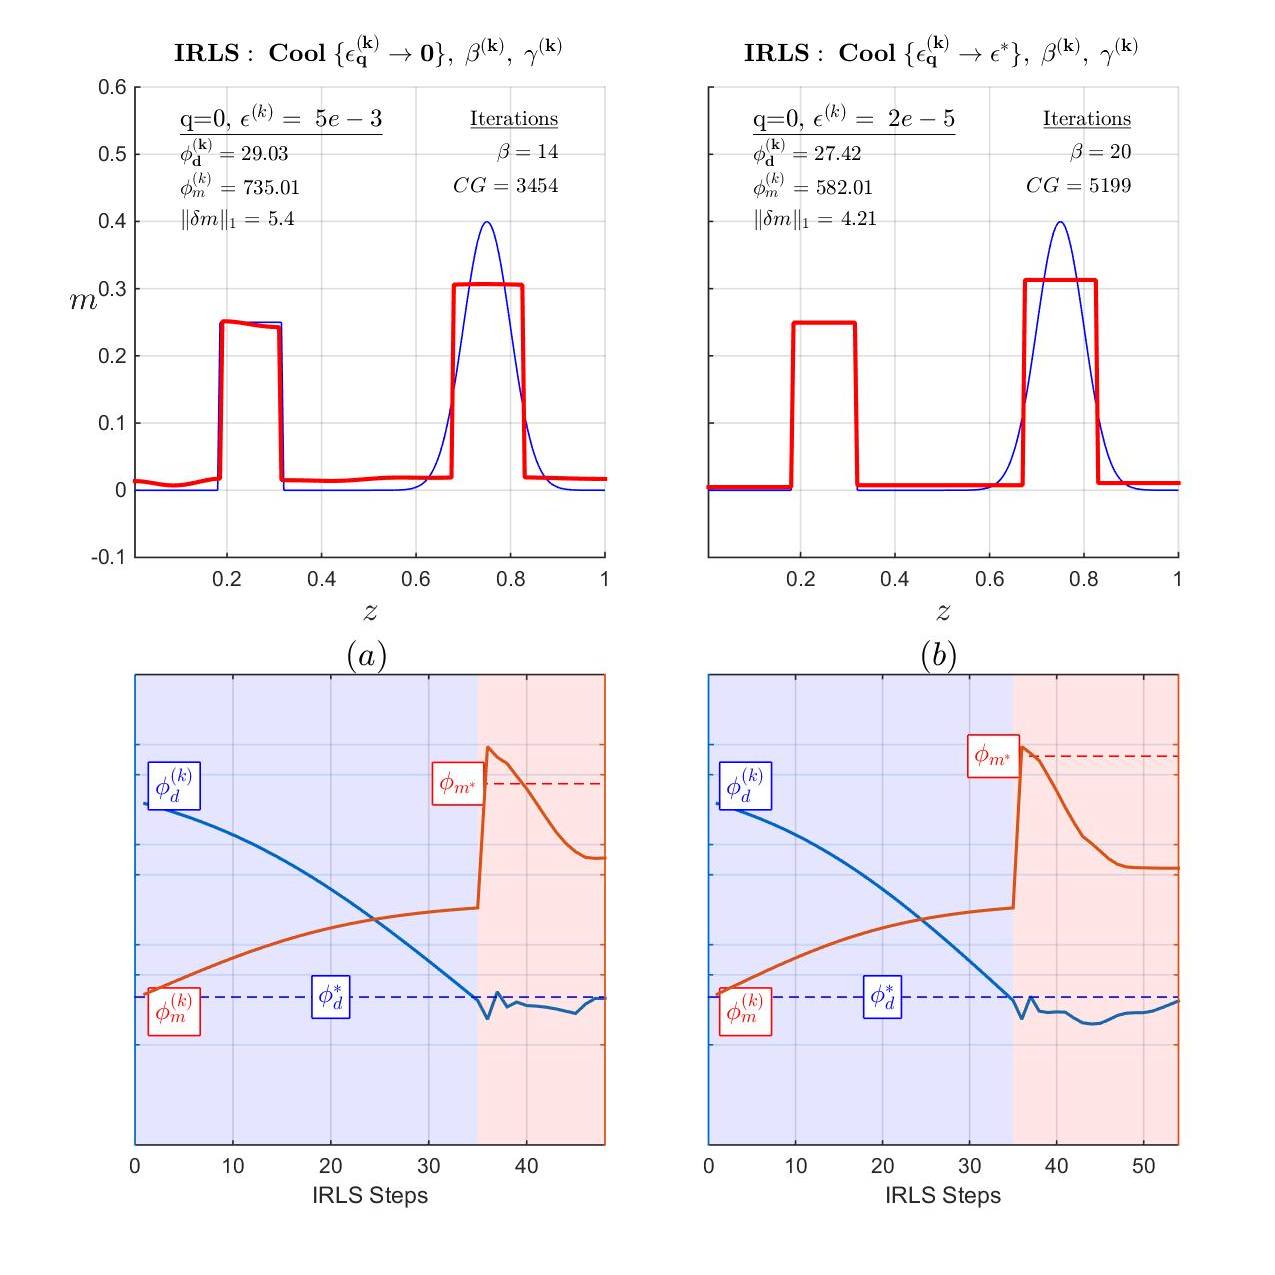
\includegraphics[scale=0.57]{1D_IRLS_algo3}
\caption{(Top) Recovered models from two different algorithms used to implement the IRLS method for $q=0$ with cooling of the threshold parameter $\epsilon$. (Bottom) Measure of model misfit and model norm as a function of iterations. Both algorithms adjust $\beta$ and scaling parameter $\gamma^{(k)}$ between each IRLS iteration. (a) In the first case, the threshold parameter $\epsilon$ is monotonically reduced until reaching the convergence criteria. The solution is sparser than the previous algorithm, even though $\epsilon$ is much larger than machine error.
(b) In the second case, $\epsilon$ is decreased until reaching the target threshold $\epsilon^*$. The solution is blocky, penalizing small model gradients.}
\label{fig:1D_IRLS_algo3}
\end{figure}

The method proposed above is advantageous as it does not require a specific choice of threshold parameters $\epsilon_p$ and $\epsilon_q$.
It does depend however on the specified convergence criteria $\delta \phi_m^{(k)}$.
In some cases, the algorithm may converge too quickly before reaching the desired level of sparsity. 
Alternatively, the algorithm may become overly expensive if the convergence criteria is too restrictive or the solution oscillates around the minimum. 
Secondly, the stabilizing parameter $\epsilon$ can be interpreted as an $effective\;zero$, penalizing specific ranges of model parameters.
It may therefore be necessary to determine a minimum threshold value in order to guarantee convergence and penalize the right model values.

Since the initialization of the IRLS requires a good approximation of the model via a least-squares solution, an estimate of the distribution of model parameters is available for analysis.
The value of an optimal $\epsilon^*$ can be chosen directly by the user based on $a\;priori$ information. Alternatively the choice can be based on the distribution of model values.
Figure~\ref{fig:1D_Model_curve}(a) presents the distribution of model and model gradients obtained from the smooth $l_2$-norm inversion.
Both curves display a sharp corner around which the model parameters rapidly change. 
Similarly, \cite{ZhdanovTolstaya2004} suggest an L-curve based on the change in model norm such that:
\begin{equation}\label{s_ms}
\begin{split}
s_{MS}(\epsilon) &= \mathbf{m^T R_\text{s}^T R_\text{s} m} \\
s_{MGS}(\epsilon) &= \mathbf{m^T G_\text{x}^T R_\text{x}^T R_\text{x} G_\text{x} m}\;,
\end{split}
\end{equation}
where the model norm $s_{MS}$ and model gradient norm $s_{MGS}$ are computed over a range of $\epsilon$ values as shown in \ref{fig:1D_Model_curve}(b). I found experimentally that both approaches were valid but did not always yield a well defined corner.
More research may be needed to determine the most robust approach.

As a final experiment, I invert the 1-D example using the point of maximum curvature on the $s_{MGS}$ curve as a minimum threshold  for the model gradients  ($\epsilon_q^*=2e-5$) . Figure~\ref{fig:1D_IRLS_algo3}(b) presents the model after convergence.
I note that the result is more blocky than the one previously obtained with the convergence criteria.
The inversion is, computationally, slightly more expensive due to the larger number of IRLS steps to reach the target threshold parameter $\epsilon_q^*$. 


\begin{figure}[p]
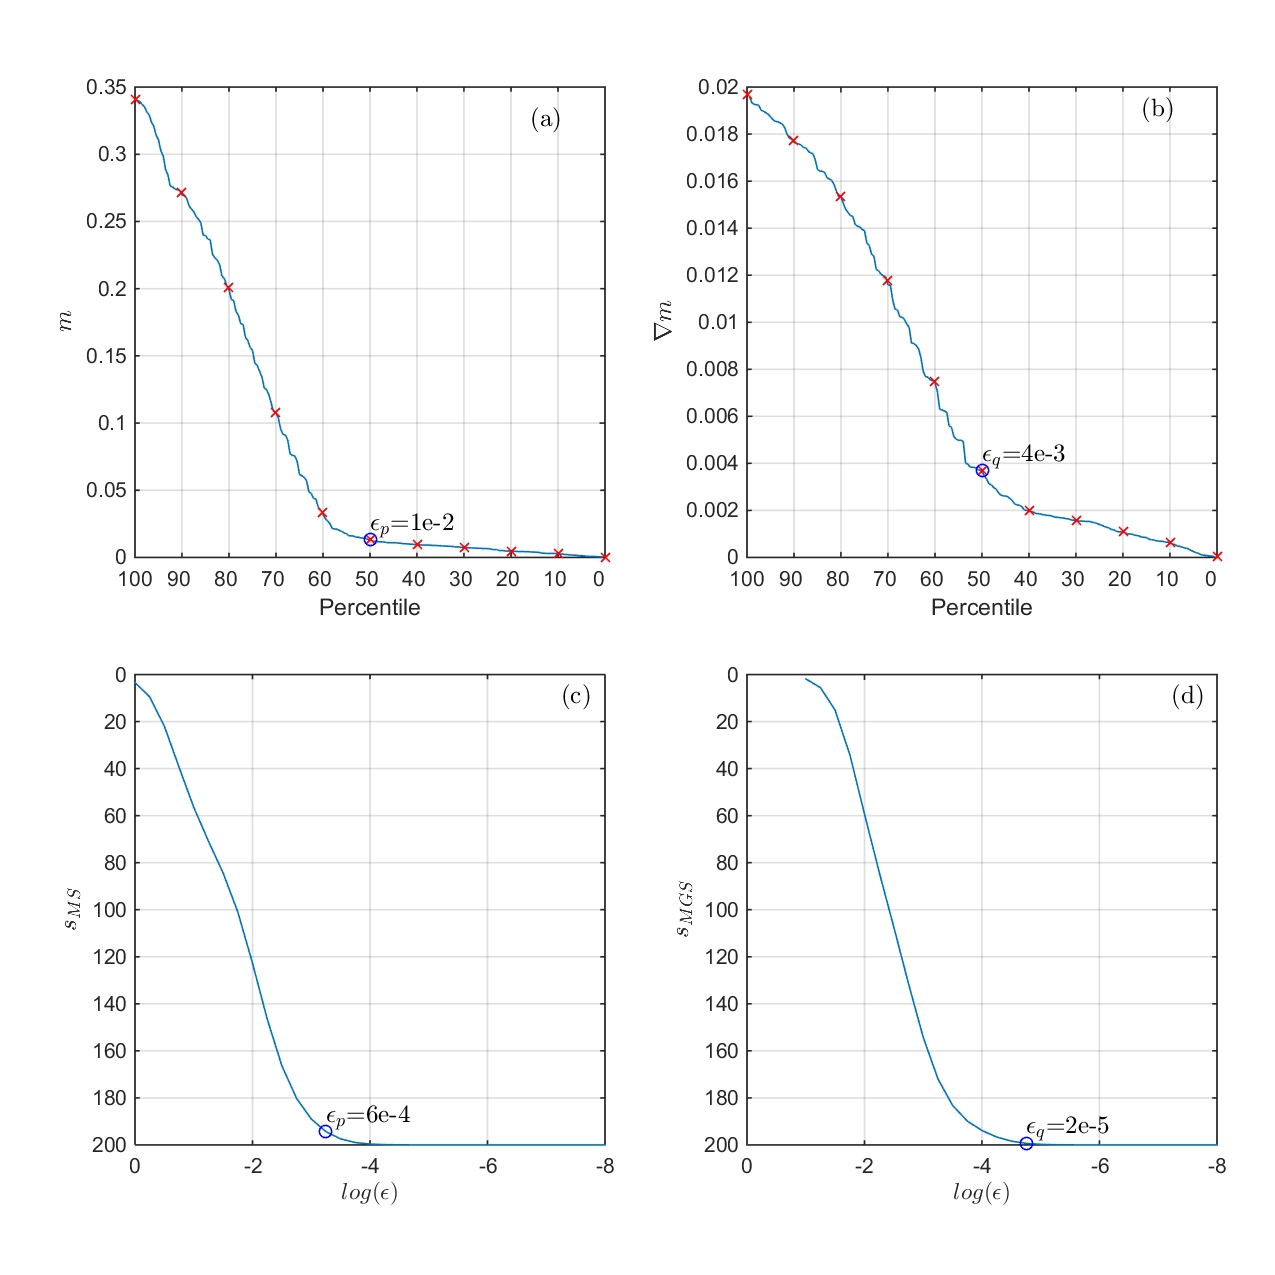
\includegraphics[scale=0.6]{1D_Model_curve}
\caption{(a) Distribution of model parameters and (b) model gradients recovered from the smooth $l_2$-norm regularization.
Both curves show a sharp corner around which the model functions vary rapidly. Similarly, a measure of (c) model norm $s_{MS}$ and (d)  model gradient norm $s_{MGS}$ can be computed over a range of $\epsilon$ values, yielding a similar $L-curve$. The point of maximum curvature can be used to determine the optimal $effective\;zero$ parameter $\epsilon_p$ and $\epsilon_q$. }
\label{fig:1D_Model_curve}
\end{figure}
%The S-IRLS algorithm can be summarized as follow:
%\begin{itemize}
%\setlength\itemsep{0em}
%\item{Phase l \textemdash $L_2$-norm initialization:} 
%\begin{itemize}
%	\setlength\itemsep{0em}	
%	\item Inversion with $l_2$-norm regularization $\rightarrow$ $\mathbf{m}^{(0)}$ , $\beta^{(0)}$
%	\item Set threshold values $\epsilon_p$, $\epsilon_q$ (see section \ref{eps_algo})
%\end{itemize}	
%\item Phase ll \textemdash S-IRLS iterations: $while \; \tau^{(k)} < 1\%$
%\begin{itemize}
%	\setlength\itemsep{0em}		
%	\item Generate IRLS weights: $\mathbf{R}_s$, $\mathbf{R}_x$
%	\item Compute gradient scales: $\eta_p$, $\eta_q$ $\rightarrow$ $\mathbf{\hat R}_s$, $\mathbf{\hat R}_x$
%	\item Compute regularization scaling: $\gamma^{(k)}$ 
%	\item Solve $\phi^{(k)}$: $\mathbf{m}^{(k)}$  $\rightarrow$ $\mathbf{m}^{(k+1)}$
%\end{itemize}
%\item Phase lll \textemdash Adjusting $\beta$: $while \; \phi_d^{(k)} \ne \phi_d^*$
%\begin{itemize}
%	\item Adjust trade-off parameter $\rightarrow$ $\beta^{(k)}$
%	\item Solve $\phi^{(k)}$: $\mathbf{m}^{(k)}$  $\rightarrow$ $\mathbf{m}^{(k+1)}$ 
%\end{itemize}
%\end{itemize}

%The S-IRLS method is non-linear with respect to the model parameter and requires several iterations before converging to stable solution.
%Just as for the Gauss-Newton steps, I need a criteria to stop the iteration process.
%During Phase ll of the algorithm, I monitor the change in distribution of model values such that :
%\begin{equation} \label{eq:dcdm}
%	\tau^{(k)} =  \frac{ | \xi^{(k)} -  \xi^{(k-1)} |}{\xi^{(k)}} \times 100
%\end{equation}
%where I define a clustering parameter $\xi$ as:
%\begin{equation}
%\begin{split}
%&\xi^{(k)} = \sum_{i=1}^M y_i  \\
%&\begin{cases} 
%y_i = 1 & if\; m_i < \epsilon \\
%y_i = 0 & if\; m_i \ge \epsilon
%\end{cases}
%\end{split}
%\end{equation}
%The clustering term $\xi$ simply measures the number of model values smaller than $\epsilon$.
%I found experimentally that monitoring the clustering of model parameters is a more robust measure of convergence than other measures such as used in Equation~\ref{Convergence}.
%For $p < 1$, only the smallest model parameters are penalized, and they may not have a big impact on the overall measure of $\|\mathbf{m}^{(k)}\|$, yet the model may still be changing around $\epsilon$. 
%Motoring the number of cells on either side of $\epsilon$ reveals if the inversion has reached a stable solution specifically for the model values targeted by the norm.  

%%%%%%%%%%%%%%%%%%%%%%%%%%%%%%%%%
\newpage
\section{Scaled-IRLS method (S-IRLS)}\label{S-IRLS}
The blocky solution found previously is expected from an $l_0$-norm penalty on the gradient. But it is clearly not appropriate to recover  the true synthetic model, which is both smooth and sparse.
Building upon the previous section, I explore different combinations of norms on the model and model gradients in order to $shape$ the penalty function. This function should allow any available $a\;priori$ information to be incorporated in the solution.
My first attempt uses an $l_0$-norm on the model combined with and $l_2$-norm on the model gradients, or $\{p=0 , q = 2\}$.
For this combination of norms, I would expect the solution to be both sparse and smooth, better approximating the width of the rectangular pulse and Gaussian anomaly.
Figure \ref{fig:1D_Eta_test}(a) shows the solution after convergence of the IRLS algorithm.
I here identify an important issue with the current IRLS method involving various norm measures within the same objective function. 
The solution is clearly dominated by the sparsity constraint. 
In this case, the $l_0$-norm penalty on the model suppresses the $l_2$-norm penalty on the model gradient, yielding a strictly sparse solution without smoothness constraint.

\begin{figure}[p]
\centering
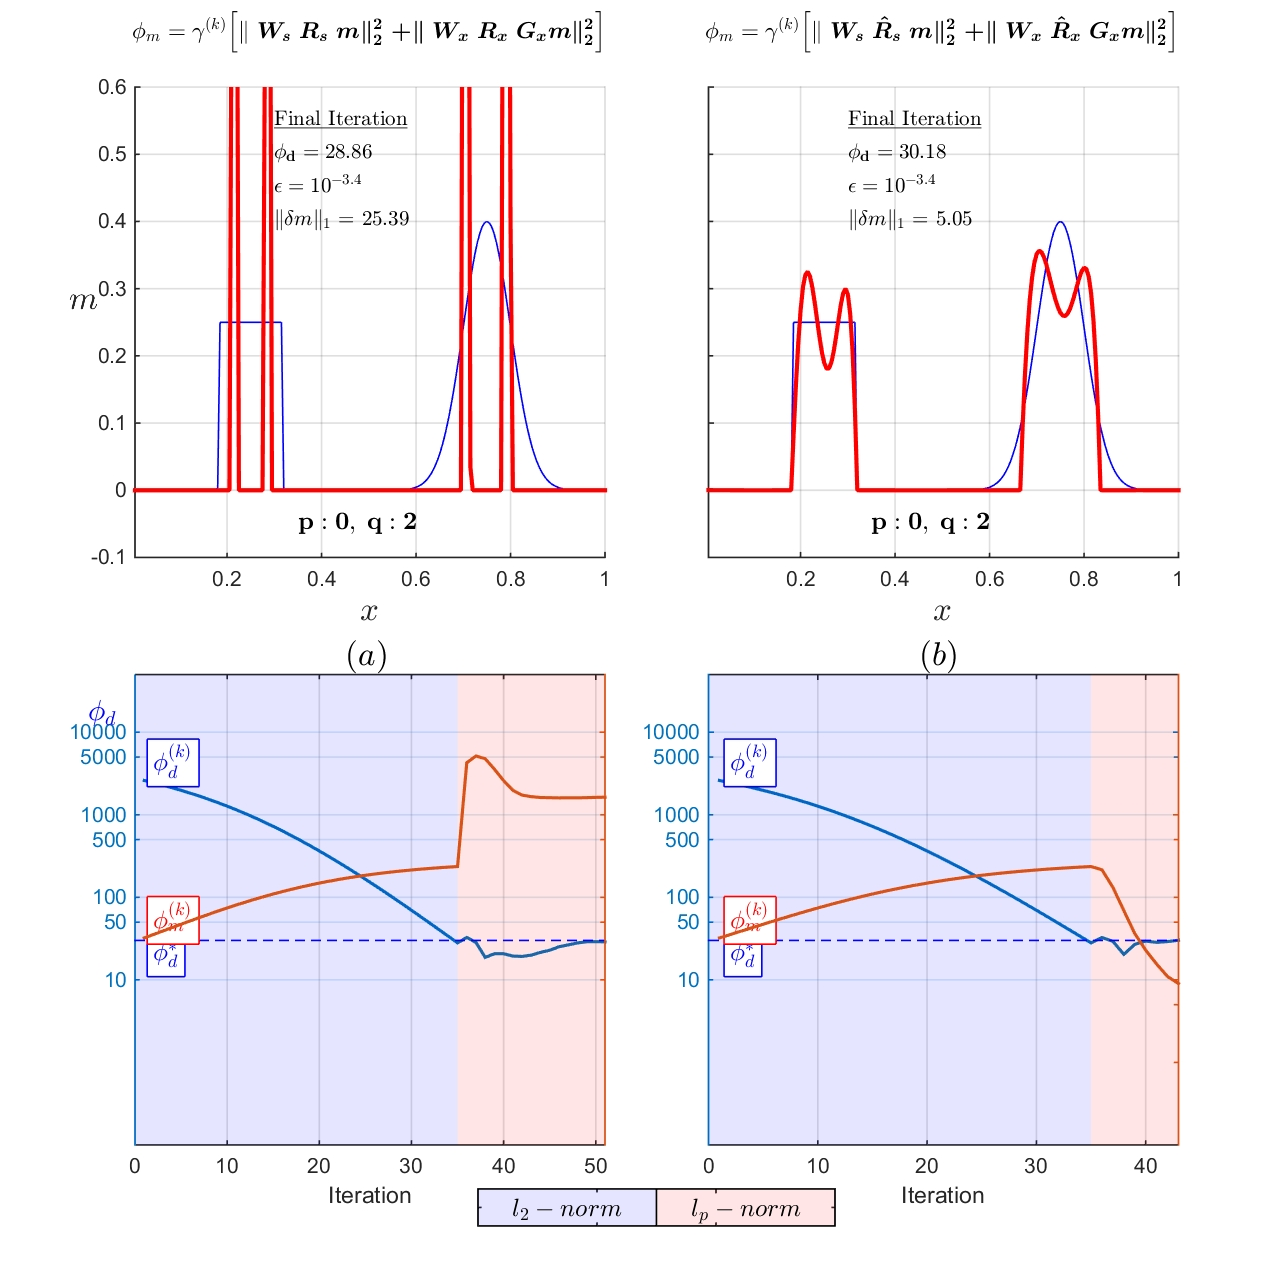
\includegraphics[scale=0.6]{1D_Eta_test}
\caption{(a) (Top) Recovered model using a mixed-norm regularization for $p=0$, $q=2$, $\epsilon=1e-3$. (Bottom) Measure of model misfit and model norm as a function of iterations. The inversion converges to a sparse solution without apparent penalty on the gradient, indicative of an imbalance in the regularization. (b) Recovered model and convergence curves after rescaling of the regularization, yielding a model that is both sparse and smooth as expected from the applied mixed-norm .}
\label{fig:1D_Eta_test}
\end{figure}

To understand the issue, it is useful to look at the linear system defined by \ref{eq:dphi_dm_lp}. 
Recall that a solution is found along the gradient of the objective function, which from \eqref{eq:dphi_dm} can be written explicitly as:
\begin{equation}\label{StepDirection}
\begin{split}
\frac{\partial \phi(m)}{\partial m} &= \big(\mathbf{F^T\;d} - \mathbf{F^T\;F\;m}\big) - \beta\big (\;  \mathbf{g_s}(m) + \mathbf{g_x}(m)\;\big ) \\
\mathbf{g_s}(m) &=  \mathbf{R_{\text{s}}^T}\; \mathbf{W_{\text{s}}^T} \mathbf{W}_s \;\mathbf{ R}_s\; \mathbf{m}\\
\mathbf{g_x}(m) &=  \mathbf{G_{\text{x}}^T} \;\mathbf{R^T}_x\; \mathbf{W_{\text{x}}^T}\mathbf{W}_x \;\mathbf{R}_x \; \mathbf{G}_x\; \mathbf{m} \;.
\end{split}
\end{equation}
I divided \eqref{StepDirection} into three parts to highlight the different components of the total gradient direction.
The first term $\big(\mathbf{F^T\;d} - \mathbf{F^T\;F\;m}\big)$ is related to the misfit function and depends solely on the ability of the model to reproduce the data $\mathbf{d}$. 
The second term $ \beta\big (\;  \mathbf{g_s}(m) + \mathbf{g_x}(m)\;\big )$ is related to the regularization function, which depends on the IRLS weights $\mathbf{R_s}$ and $\mathbf{R_x}$ computed in \ref{eq:R_w}.

To illustrate the importance of scaling between the function gradient terms I form a slightly different 2-variable problem where:
\begin{equation}
	\mathbf{F} = 
	\begin{bmatrix}
	0 & 1
	\end{bmatrix}\:,\:
	\mathbf{d} = 1 .
\end{equation}
Figure \ref{fig:IRLS_Phis_Phix}(a) displays contours along the surface formed by the $l_2$-norm measure of data residual $\|\mathbf{ F\;m - d }\|_2^2$, where this time the null-space of $\mathbf{F}$ lies parallel to the $x$-axis. 
I simplify the problem by having cell size and weights all equal to one so the objective function can be written as:
\begin{equation}\label{eq:Toy_phi}
\begin{split}
\phi(m) &= \phi_d + \beta \left[ \phi_s + \phi_x \right] \\
&= \|\mathbf{Fm - d}\|_2^2 + \beta \left [ {\| \mathbf{m}\|}^2_2 +  {\|  \mathbf{ G_\text{x} \; m}\|}^2_2  \right ] \;.
\end{split}
\end{equation}
By setting a small trade-off parameter ($\beta = 1e-3$), I can focus on the solution space along the null-space of \textbf{F} marked by the red dash line, as shown in Figure \ref{fig:IRLS_Phis_Phix}(e).
The global minimum of the objective function lies at $\mathbf{m} = [0.5;1]$, where the partial gradients of $\frac{\partial\phi_s}{\partial\;m_1}$ and $\frac{\partial\phi_x}{\partial\;m_1}$ have equal and opposite signs.
Here the two regularization functions use an $l_2$-norm measure, hence the optimal solution is at mid-distance from their respective minimums.
This simple example shows that the actual value of the individual norms do not matter, but rather the relative magnitude of the gradients along the  minimum of $\phi_d$.

\begin{figure}[h!]
\centering
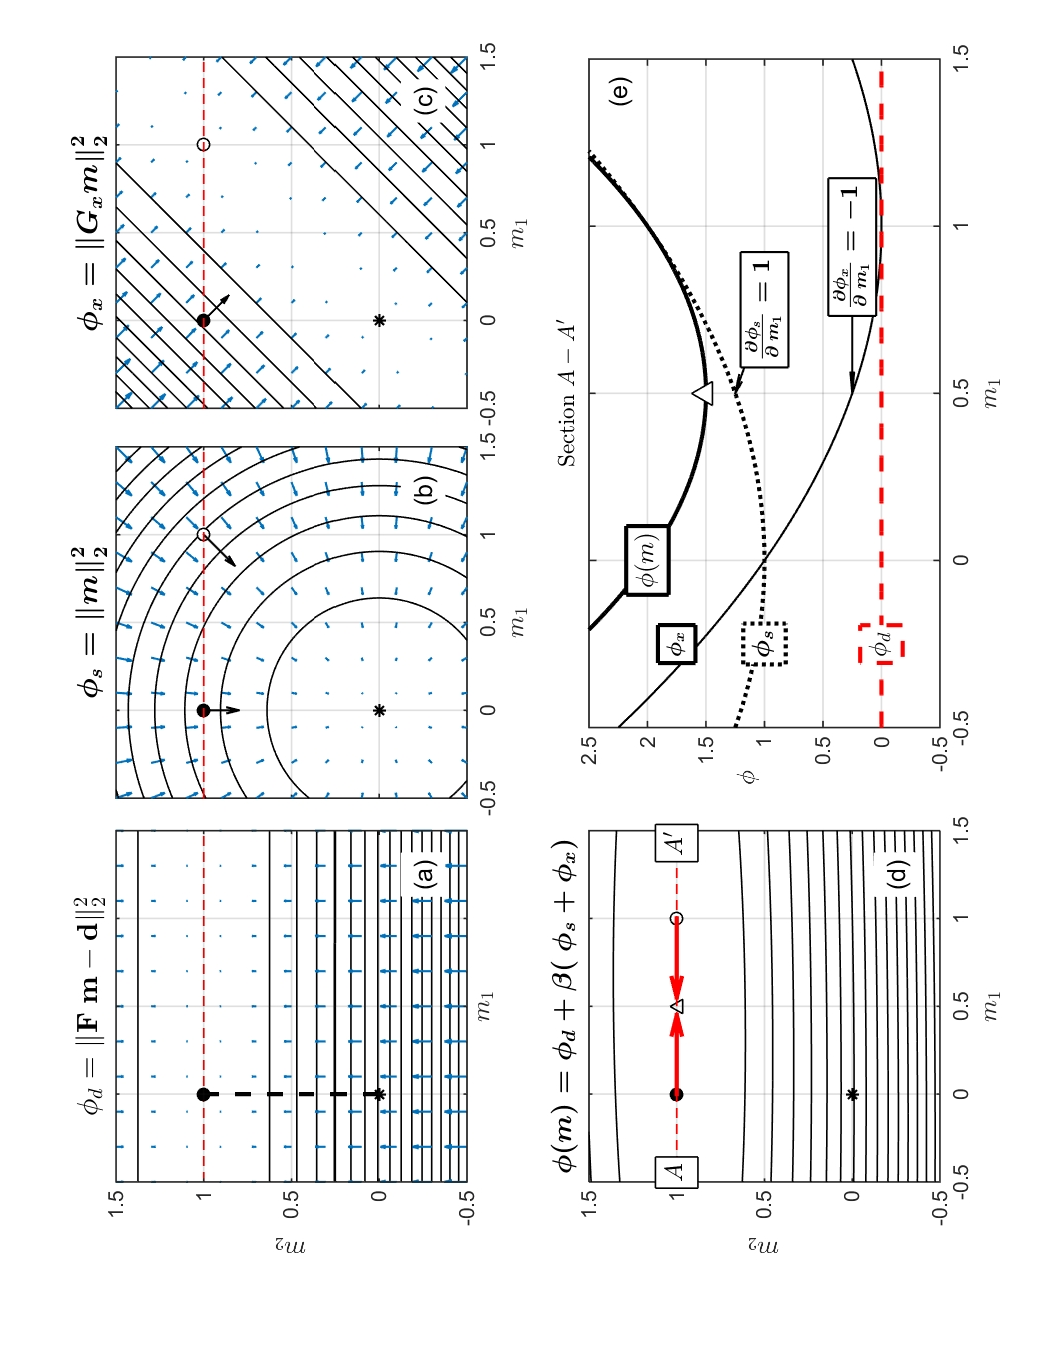
\includegraphics[scale=0.55, angle=270]{IRLS_toy_Phis_Phix}
\caption{Contour maps for (a) the misfit function $\phi_d$, (b) the model norm $\phi_s$ and (c) the norm of model gradients $\phi_x$. (d) The total objective function $\phi(m)$ has a global minimum located at $\mathbf{m}=(0.5,1.0)$ for a given small trade-off parameter ($\beta = 1e-3$). The direction of update is shown for two starting models $\mathbf{m}^{(0)}$ (black and white dot). (e) Section through the objective function along the minimum of $\phi_d$. The global minimum occurs where the partial gradients of $\frac{\partial\phi_s}{\partial\;m_1}$ and $\frac{\partial\phi_x}{\partial\;m_1}$ have equal and opposite signs.}
\label{fig:IRLS_Phis_Phix}
\end{figure}

The behavior of the $l_0$-norm for small $p$ and $\epsilon$ values can easily explain the result obtain in Figure~\ref{fig:1D_Eta_test}(a).
Figure~\ref{fig:Lp_g_scaled}(a) compares the function gradients for different norm penalties as a function of $p$ values. 
In this case, the function gradients $\mathbf{g_s}$ measured with the $l_0$-norm are always much larger than the function gradients $\mathbf{g_x}$ measured with the $l_2$-norm, except at $m_i = \{0, \sqrt{1-\epsilon^2}\}$.
The solution can therefore only be sparse with few non-zero model values required to satisfy $\phi_d^*$. 
The penalty on model gradients had no influence on the solution.

Just as I added the parameter $\gamma^{(k)}$ to balance the relative importance between the misfit function and the regularization, I also want to control the relative scaling between the various regularization functions in terms of their gradients.
In other words, I want to find a scaling parameter that makes the gradient of any $l_p$-norm function to intersect, elsewhere than at $m_i = \{0, \sqrt{1-\epsilon^2}\}$.

I here introduce a scaling parameter $\eta$:
\begin{equation} \label{eq:eta}
\eta =  \epsilon^{(1-p/2)} \;,
\end{equation}
where once again $p$ denotes the $l_p$-norm penalty and $\epsilon$ is a small value used to approximate the norm.
Adding the scaling parameter $\eta$ to \ref{eq:dphidm}, the partial gradients of the objective function  become:
\begin{equation} \label{S-lp_dphidm}
\frac{\partial \phi_m}{\partial m} = \;\frac{\epsilon^{(1-p/2)}  x_i}{{{(x_i}^{2} + \epsilon^2 )}^{1-p/2}}  \;.
\end{equation}

\begin{figure}[h!]
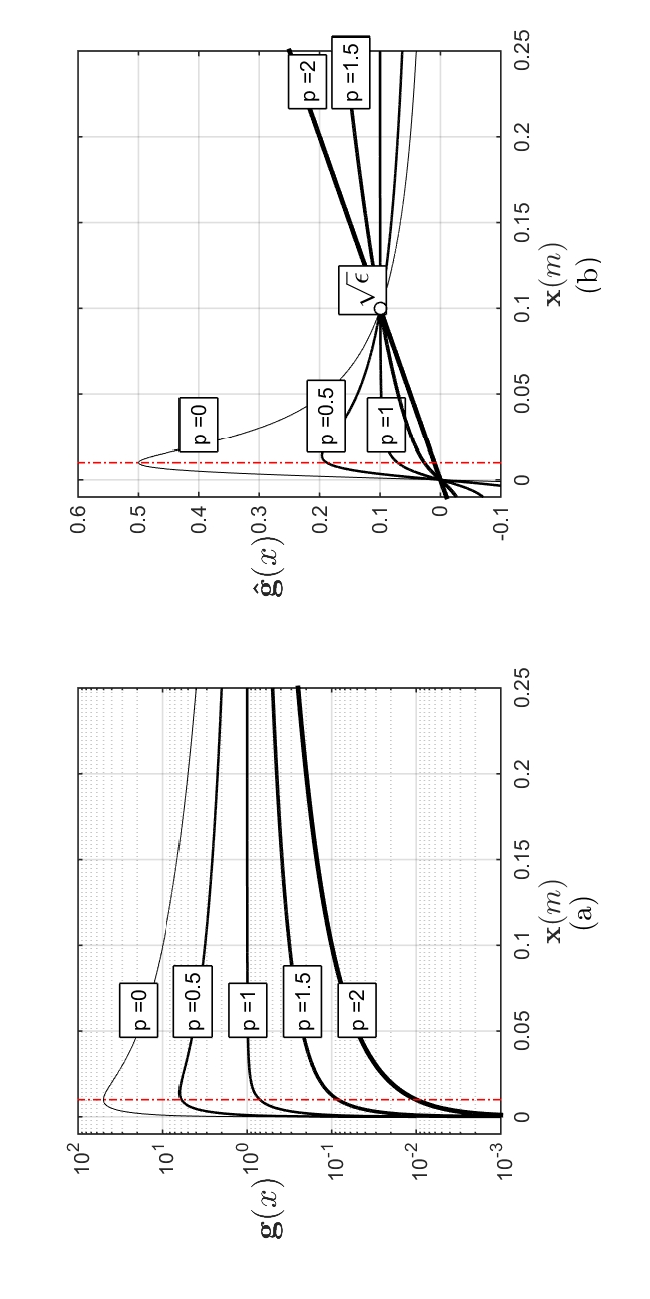
\includegraphics[scale=0.58,angle=270]{Lp_g_scaled}
\caption{(a) Partial gradients of approximated $l_p$-norm penalties for a fix stabilizing parameter $\epsilon =1e-2$. Gradients for $p < 1$ are consistently larger on the interval $[0 < x_i < \sqrt{1-\epsilon^2}]$, making it hard to combine multiple norm penalties within the same objective function. (b) Function gradients after applying a scale of $\epsilon^{(1-p/2)}$, forcing each $l_p$-norm to intersect at $m = \sqrt{\epsilon}$.   }
\label{fig:Lp_g_scaled}
\end{figure}

Looking at the gradient for $x_i=\sqrt{\epsilon}$, \ref{S-lp_dphidm} simplifies to:
\begin{equation*}
\frac{\partial \phi_m}{\partial m} = \;\frac{\epsilon^{1/2}}{{(1+ \epsilon )}^{1-p/2}} \;.
\end{equation*}
Then assuming that $\epsilon \ll 1$:
\begin{equation} \label{approx_lp}
\frac{\partial \phi_m}{\partial m}\approx \; \epsilon^{1/2} \;.
\end{equation}
Hence after applying the scaling $\eta$, the gradient of the $l_p$-norm is independent of the $p$-value exactly at $m=\sqrt{\epsilon}$, and has also a gradient $\frac{\partial \phi}{\partial m}=\sqrt{\epsilon}$, as shown in Figure~\ref{fig:Lp_r_dphidm}(c).
Therefore, $\sqrt{\epsilon}$ is a critical point around which all norm penalties can influence the solution.
In this manner, two penalty functions with different $p$-values can coexist within a regularization function and achieve different objectives.
 
 Adding this final scaling to \ref{eq:scaled_Lp_phi} yields a \emph{Scaled Iterative Re-weighted Least Squares} (S-IRLS) regularization function such that: 
\begin{equation} \label{eq:S-IRLS}
\hat \phi_m^{(k)} = \gamma^{(k)} \Big ( {\| \mathbf{W_\text{s} \; \hat R_\text{s} \; m}\|}^2_2 +  {\|  \mathbf{ W_\text{x}\; \hat R_\text{x} \; G_\text{x} \; m}\|}^2_2  \Big ) \;.
 \end{equation}
I define a Scaled-IRLS weighting matrix $\mathbf{\hat R}$ such that:
\begin{equation} \label{eq:eta}
\begin{split}
{\hat R}_{s_{ii}}  &= \sqrt{\eta_p}{\Big[ {({m_i}^{(k-1)})}^{2} + \epsilon_p^2 \Big]}^{(p/2 - 1)/2} \\
{\hat R}_{x_{ii}}  &= \sqrt{\eta_q}{\Big[ {\left ({\frac{\partial m_i^{(k-1)} }{\partial x}}\right)}^{2} + \epsilon_q^2 \Big]}^{(q/2 - 1)/2}  \\
\eta_p &=  {\epsilon_p}^{(1-p/2)} \\
\eta_q &=   {\epsilon_q}^{(1-q/2)}  \;, 
\end{split}
\end{equation}
where $\epsilon_p$ and $\epsilon_q$ are the stabilizing parameters for the $l_p$-norm of the model and model gradients respectively.
Note that for $p=2$, the scaling parameters $\eta$ is equal to one, hence we recover the the classic $l_2$-norm regularization. 

 Figure \ref{fig:1D_Eta_test}(b) presents the result after a re-scaling of the gradient descent. 
Both the $l_0$-norm penalty on the model and the $l_2$-norm penalty on the model gradients are represented, yielding a solution that is both sparse and smooth. 
I now have a flexible and robust regularization function. This allows us to explore a wide range of solutions, or $l_p$-space of solutions, combining various norms on the model and model gradients.

\subsection{Cell-based weights (${w}_r,\; w_m$)}\label{Wr_Section}
In \cite{LiOldenburg1996}, a depth weighting function is added to counter the natural decay of potential fields. 
The rapid decay in sensitivity is an important problem in geophysics as most data sets are acquired from the surface.
The same idea can be used to incorporate any \emph{a priori} information regarding the spatial distribution of model parameters.
In this section, I investigate the effect of having such cell-based weighting applied directly to the sensitivity matrix, compared to having it applied to the regularization function as previously formulated in \ref{eq:Phi_disc} .

Following the weighted sensitivity formulation of \cite{LiOldenburg1996}, the objective function with S-IRLS regularization takes the form:
\begin{equation} \label{eq:phi_Wrm}
 \phi(\hat m) = \|\mathbf{W_d \;(\hat F\; \hat m - d)}\|_2^{2} + \gamma^{(k)} \Big [ {\|\mathbf{W_\text{s}  \;\hat R_\text{s} \; \hat m}\|}^2_2  +   {\|\mathbf{  W_\text{x}  \;\hat R_\text{x} \; G_\text{x} \; \hat m}\|}^2_2  \Big ] \;,
 \end{equation}
 where:
\begin{equation*}
\begin{split}
\mathbf{\hat F} &= \mathbf{F\;W_\text{r}^{-1}} \\
\mathbf{\hat m} &= \mathbf{W_\text{r}\;m} \\
\mathbf{W_\text{r}} &= diag \left( e^{j\: z / (2 \pi)} \right )\;,
\end{split}
\end{equation*}
where the matrix $\mathbf{W_\text{r}}$ hold the inverse exponential describing the decay of the kernel functions presented in \ref{eq:kernel_1D}.  
Similar sensitivity based weighting is used in the \textit{Minimum Support} functional of \cite{PortniaguineZhdanov02}.

Using both formulations, I invert the same 1-D example presented in Figure\ref{fig:1D_IRLS_algo3} and \ref{fig:1D_Eta_test}.
In the first experiment, I apply a sparsity constraint on the model gradients for $q=0, \alpha_s =0$. 
Figure \ref{fig:1D_Wr_in_vs_out}(a) compares the true and recovered models after convergence.
I observe the solution obtained with the $\phi({\hat m})$ formulation is skewed in the direction of the sensitivity weighting.
Similarly, Figure \ref{fig:1D_Wr_in_vs_out}(b) shows the recovered model for the combination of $p= 0,\;q=2$.
While the recovered anomaly over the rectangular pulse is both smooth and sparse, I note that the solution tends to favor a strictly sparse model further at depth over the Gaussian function.
On the other end, the solution obtained with the $\phi({m})$ formulation remains smooth and sparse over both anomalies equally.

Issues encountered with the $\phi({\hat m})$ formulation are due to the IRLS weights computed in \ref{eq:Rs_Rx}.
Written explicitly in terms of weighted model parameters, the linearized IRLS norm from \ref{eq:IRLS_phi} can be written as:
\begin{equation}\label{Weighted_IRLS}
\phi_{\hat m}^{(k)} =  \sum^{nc}_{i=1} \frac{{(w_i x_i)}^2}{ {\left[{(w_i x_i^{(k-1)})}^2 + \epsilon^2 \right ]}^{1-p/2}} \;.
\end{equation}
Factoring out the cell-based weight $w_i$, equation~\ref{Weighted_IRLS} becomes:
\begin{equation}\label{Weighted_IRLS_Facto}
\phi_{\hat m}^{(k)} =  \sum^{nc}_{i=1}  \frac{w_i^p x_i^2}{ {\left[{(x_i^{(k-1)})}^2 + \epsilon^2/w_i^2 \right ]}^{1-p/2}} \;.
\end{equation}
The important point to note is that the weights are now function of the $p$-value, while the threshold parameter $\epsilon$ depends on the cell-based weights.
In most cases, the sensitivity weights increase with distance from the observation location, which in turn reduce the threshold parameter $\epsilon$ and increase the influence of sparse norms.
This explains the increase in sparsity constraint with distance as observed in Figure~\ref{fig:1D_Wr_in_vs_out}.
In order to preserve the character of cell-based weights, it is important to isolate their effect from the $l_p$-norm penalty.
The same idea extends to any type of cell-based weights (i.e. volumetric, \emph{a priori}).
In the following chapter, various norm measures will be used simultaneously on the model and model gradient.
The predictability and stability of the algorithm depends greatly on the scaling between the various components of the objective function.

\begin{figure}[h!]
\centering
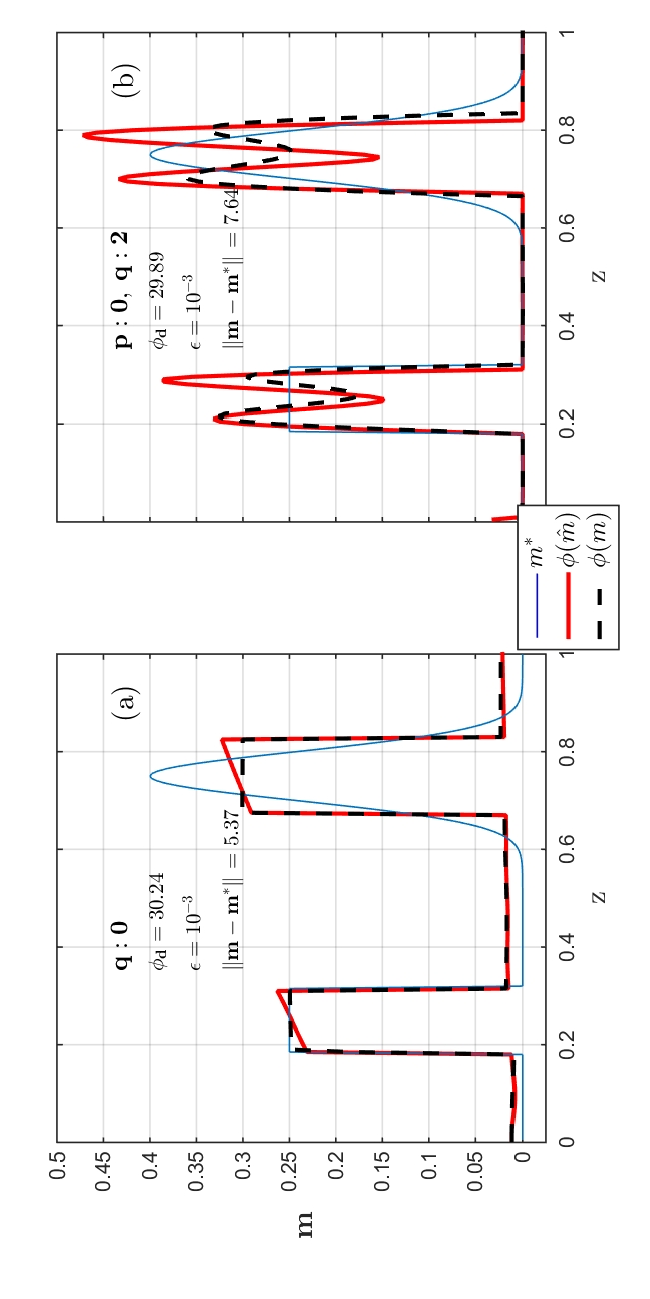
\includegraphics[scale=0.55, angle=270]{1D_Wr_in_vs_out}
\caption{Recovered models for two different depth weighting  formulations: (red)  weighted sensitivity $\phi(\hat m)$,  (black)  weighted regularization $\phi(m)$.
(a) True and recovered models using the $\phi(\hat m)$ and $\phi(m)$ formulations for penalty applied on the model gradients for $q=0$ and (b) for $p= 0,\;q=2$.
The weighted sensitivity formulation $\phi(\hat m)$ increases the influence the regularization function with distance along the $x$-axis, skewing the model towards the right.}
\label{fig:1D_Wr_in_vs_out}
\end{figure}

\newpage
%%%%%%%%%%%%%%%%%%%%%%%%%%%%%%%%%%%%%%%%%%%%%%%%%%
\section{Mixed $l_p$-norm regularization}
I showcase the robustness and flexibility of the S-IRLS algorithm by inverting a total of 441 models, corresponding to all the combinations of norms on the interval $0 \leq p \leq 2$ and $0 \leq q \leq 2$, on a 0.1 increment.
Figure \ref{fig:1D_Results_ALL}(a) presents a contour map of the final model errors $\|\delta\mathbf{m}\|_1$ recovered after each inversion.
The gradual variation in model error is a good indicator of the predictability of the algorithm, as small changes in the regularization yield equivalently small changes in the solution.
For each inversion, the trade-off parameter $\beta$ was adjusted to fit within $\pm 2\%$ of the target data misfit for appropriate comparison of the results, as shown in \ref{fig:1D_Results_ALL}(b). 
In this case, the optimal model is found with a combined norm of  [$p=1.5$,  $q=0.4$]. 
In this particular case, the worst recovery was obtained with $p=0,\; q=2$, yielding a sparse solution with few large oscillations.
Even though this type of analysis would be computationally prohibitive for large scale inverse problems, it illustrates the flexibility of the S-IRLS method in designing an objective function reflecting specific characteristics. 

Nine of the inverted models are shown in Figure \ref{fig:1D_Results} for comparison. 
As expected from the property of the IRLS functions, small norms on the gradient promote blocky solutions. From right to left, the inversion result tends to favor right-angled anomalies. From bottom to top, smaller norms on the model parameter enforce sparse solutions with few non-zero values.

\begin{figure}[p]
\centering
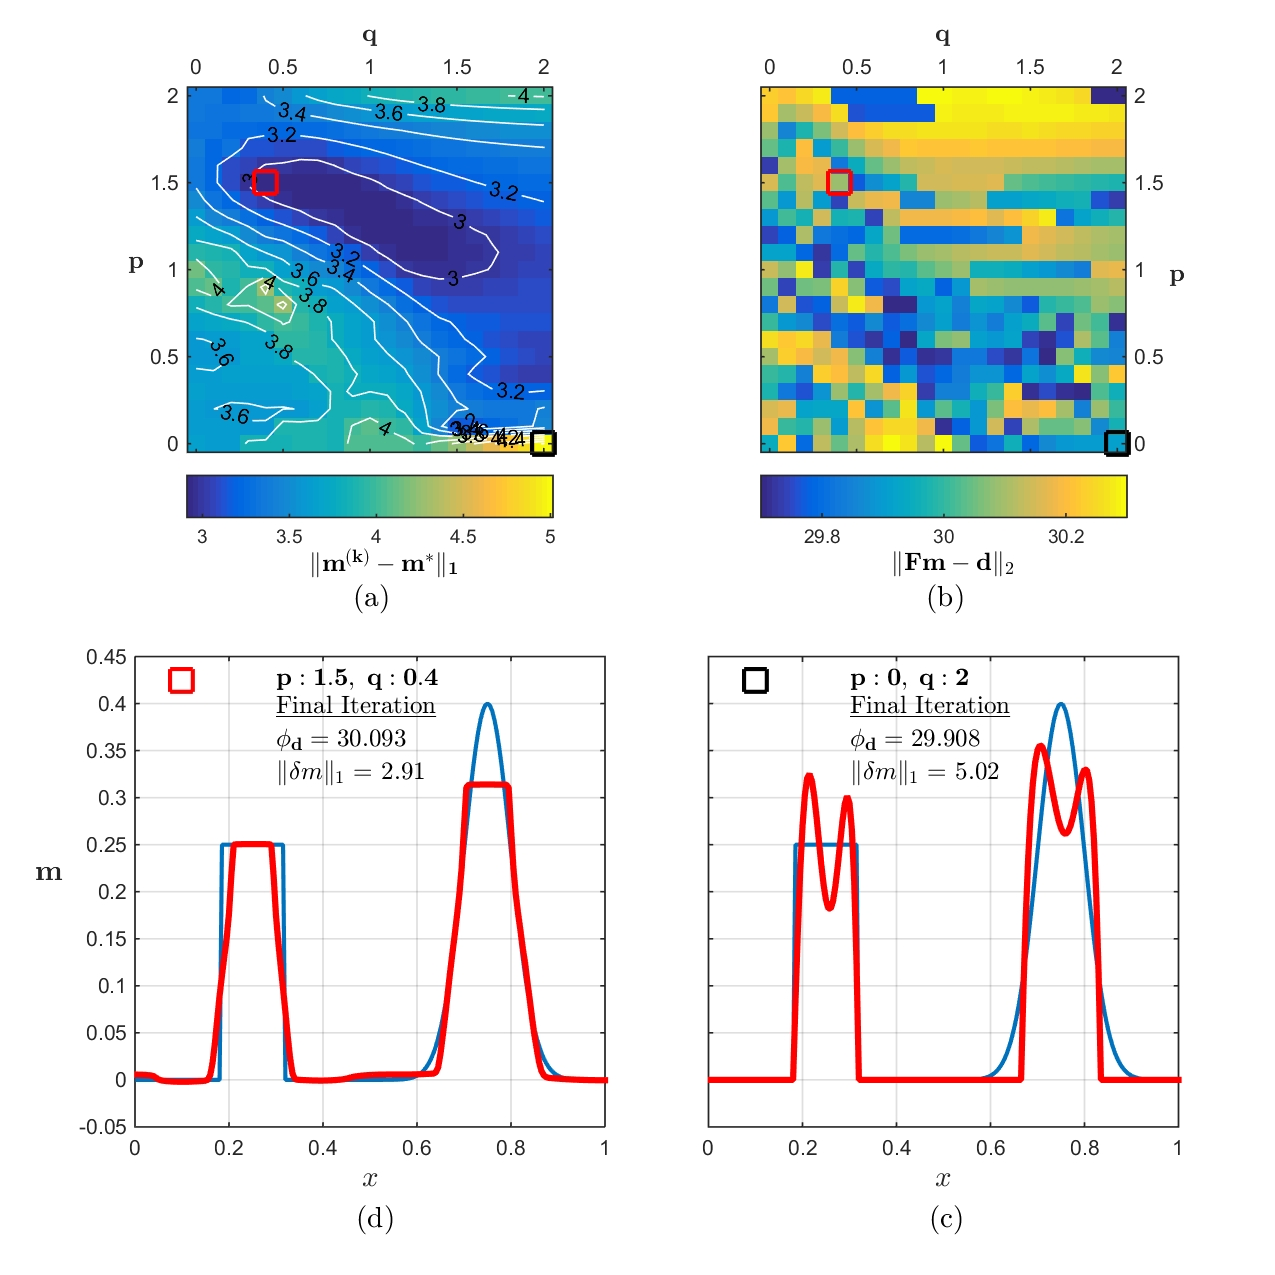
\includegraphics[scale=0.62]{1D_Results_ALL}
\caption{(a) Model error $\| m - m{*}\|_1$ and (b) misfit function for the 441 inverted models using a range of regularization with mixed-norm penalty on the model for $0 \leq p \leq 2$ and on model gradients for $0 \leq q \leq 2$. (c) The largest model error ($\| \delta \mathbf{m}\|_1$) was obtained with the mixed-norm for $p=0,\;q=2$, compared to (d) the optimal solution found with $p=1.5$ and $q=0.4$.}
\label{fig:1D_Results_ALL}
\end{figure}

\begin{figure}[t]
\centering
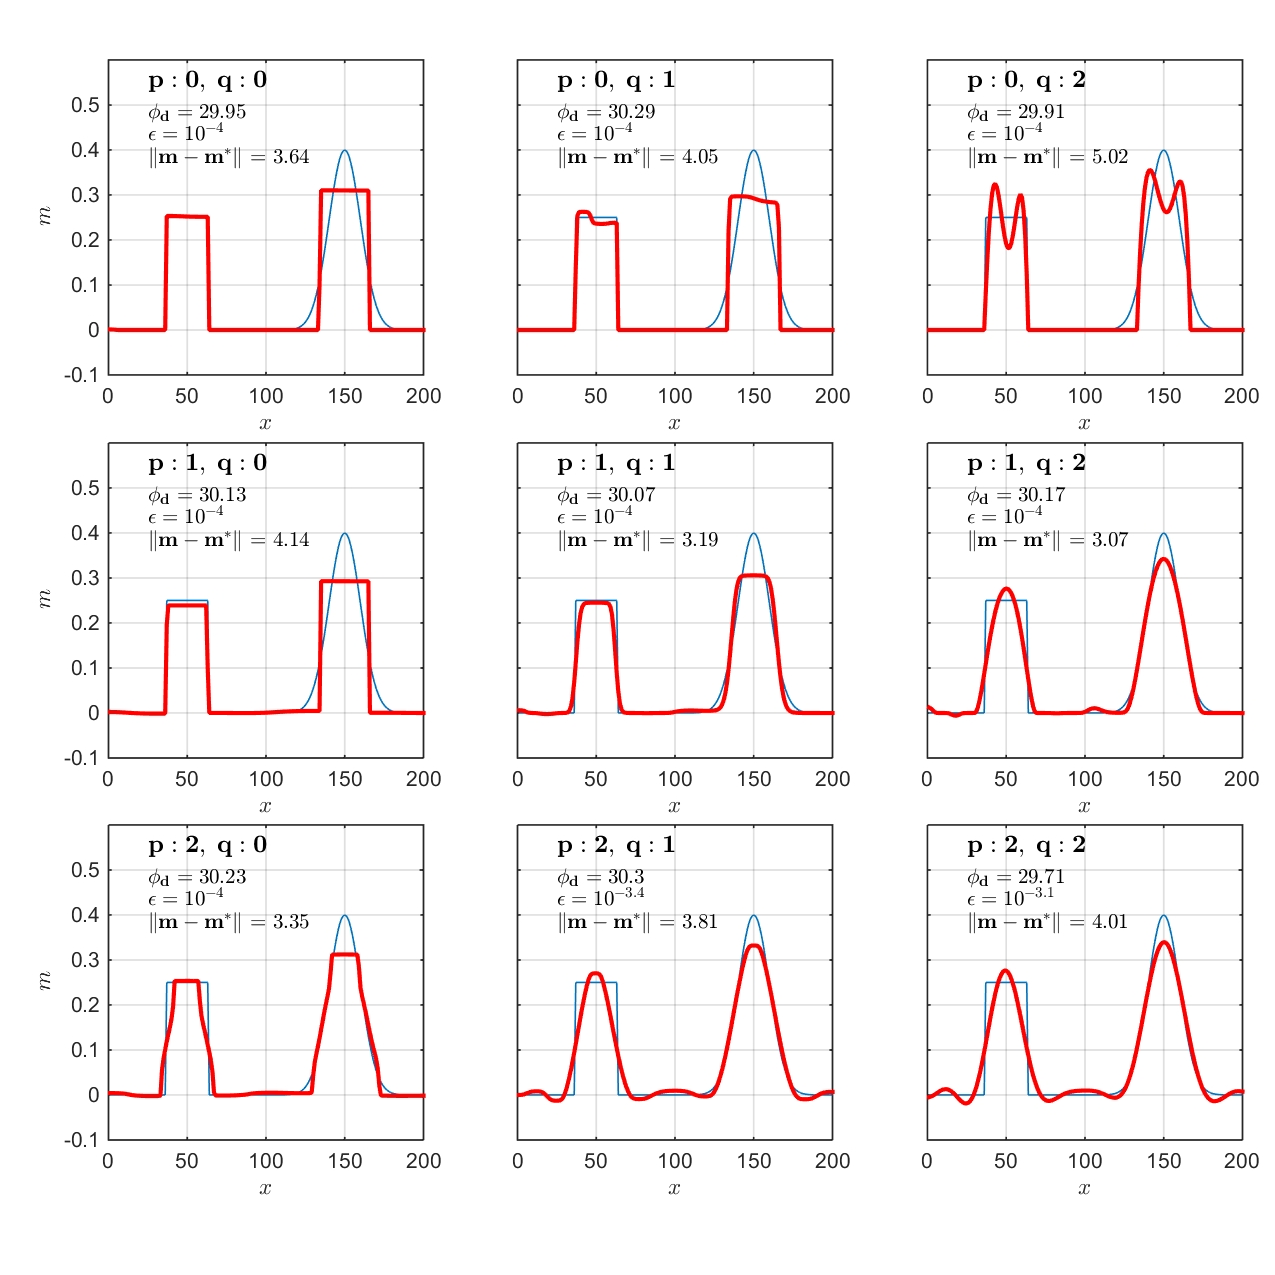
\includegraphics[scale=0.6, trim= 0.5cm 0 0 0]{1D_Results}
\caption{(a) Nine of the 441 inverted models for a range of mixed-norm penalties on the model and its gradient for $0 \leq p \leq 2$ and $0 \leq q \leq 2$. }
\label{fig:1D_Results}
\end{figure}

%%%%%%%
\subsection{Localized S-IRLS}\label{Localized_lp}
While I have so far implemented global regularization functions applied on the entire model, the S-IRLS method can easily be extended to problems made up of several sub-regions with varying norm penalties. Also based on the IRLS method, \cite{SunLi14} introduce an automated process to extract structural information from the data and impose either an $l_1$ or $l_2$-norm penalties to specific regions of the model.  
While designing this objective function can be challenging and may still require direct input from the user, their approach has great value as it increases the flexibility over traditional global penalty functions. 
The S-IRLS formulation has the potential to further generalize the work of \cite{SunLi14} in allowing the use of any norm penalty in the range of $0 \leq p \leq 2$. 

Suppose an N-dimensional model space $\mathbf{m} \in \Omega$, divided in $J$ sub-regions such that:
\begin{equation*}\label{eq:Subsets}
\begin{split}
	\mathbb{S} & = \{S_1, S_2, ... , S_J \;\Big| \;S_j \subset \Omega\ \;,\; j = 1,...,J\} \\
	S_i \cap S_j &=  \{\emptyset \;\Big| \;i,j = 1,...,J \;,\; j \neq i\}\;.
\end{split}
\end{equation*}
I can define a $model$ of $l_p$-norms by the union of each sub-domain:
\begin{equation}\label{p_vector}
\mathbf{p} = \bigcup_{j=1}^J S_j\;p_j\;,
\end{equation}
where the scaler $p_j$ defines the $l_p$-norm to be applied to the $j^{th}$ region of the model domain. 
Each sub-domain $S_j$ can have a distinct value for $p$ and $q$, penalizing the model values and model gradient differently than neighboring domains.
The transition in $l_p$-norm penalty can be smoothed after applying a linear transition across neighboring domains as defined by:
\begin{equation}\label{smooth_p_vector}
\begin{split}
\mathbf{\tilde p} &= \mathbf{A\;p} \\
\mathbf{A} &= 
		\begin{bmatrix}
			1/2 		& 		1/2	&  	0		& \dots  		&  0 \\
			\vdots	&  		 \ddots	&  	&   &  0\\
			0 		& 	\dots		& 		0	& 1/2 &  1/2 
		 \end{bmatrix} \;,
		 \end{split}
\end{equation}
where the transition between $l_p$-norm is extended over several cells by applying the averaging operator $\mathbf{A}$.
Allowing for multiple sub-domains requires only a slight change to the S-IRLS method presented in Section~\ref{S-IRLS}.
The general objective function for a 3-D discretized problem becomes:
 \begin{equation} \label{eq:Phi_IRLS}
\phi(m) =  \phi_d + \beta \gamma^{(k)} \Big [ {\| \mathbf{W}_s\;  \mathbf{\hat R}_s \;( \mathbf{m - m^{ref}})\|}^2_2  + \sum_{i = x,y,z}  {\|   \mathbf{W}_i \;  \mathbf{\hat R}_i  \; \mathbf{G}_i \; \mathbf{m}\|}^2_2  \Big ]\;,
\end{equation}
 such that the S-IRLS weights for the model and model gradients become:
\begin{equation}
\begin{split}
{\hat R}_{s_{ii}}  &= \sqrt{\tilde \eta_{p_i}}{\Big[ {({m_i}^{(k-1)})}^{2} + \epsilon^2_{p} \Big]}^{({\tilde p_i}/2 - 1)/2} \\
{\hat R}_{x_{ii}}  &= \sqrt{\tilde \eta_{q_{xi}}}{\Big[ {\left ({\frac{\partial m_i^{(k-1)} }{\partial x}}\right)}^{2} + \epsilon_q^2 \Big]}^{({\tilde q_{xi}}/2 - 1)/2}  \\
{\hat R}_{y_{ii}}  &= \sqrt{\tilde \eta_{q_{yi}}}{\Big[ {\left ({\frac{\partial m_i^{(k-1)} }{\partial y}}\right)}^{2} + \epsilon_q^2 \Big]}^{({\tilde q_{yi}}/2 - 1)/2}  \\
{\hat R}_{z_{ii}}  &= \sqrt{\tilde \eta_{q_{zi}}}{\Big[ {\left ({\frac{\partial m_i^{(k-1)} }{\partial z}}\right)}^{2} + \epsilon_q^2 \Big]}^{({\tilde q_{zi}}/2 - 1)/2}  \;.
 \end{split}
\end{equation}
Figure \ref{fig:1D_Mixed_norm} presents an optimal solution for the 1D problem, where I divide the model space into two regions.
The left half uses a $p=0, q=0$, whereas the right half imposes a $p=1$ and $q=2$.
The mixed-norm penalty function enforces the right characteristic to each portion of the model. 
The inversion recovers a sparse and blocky model over the rectangular pulse while at the same time managing to model the smooth Gaussian anomaly.
Consequently, the model error $\|\delta m\|$ is much smaller than any of the previous attempts.
The algorithm converges smoothly and rapidly to a stable solution.

\begin{figure}[t]
\centering
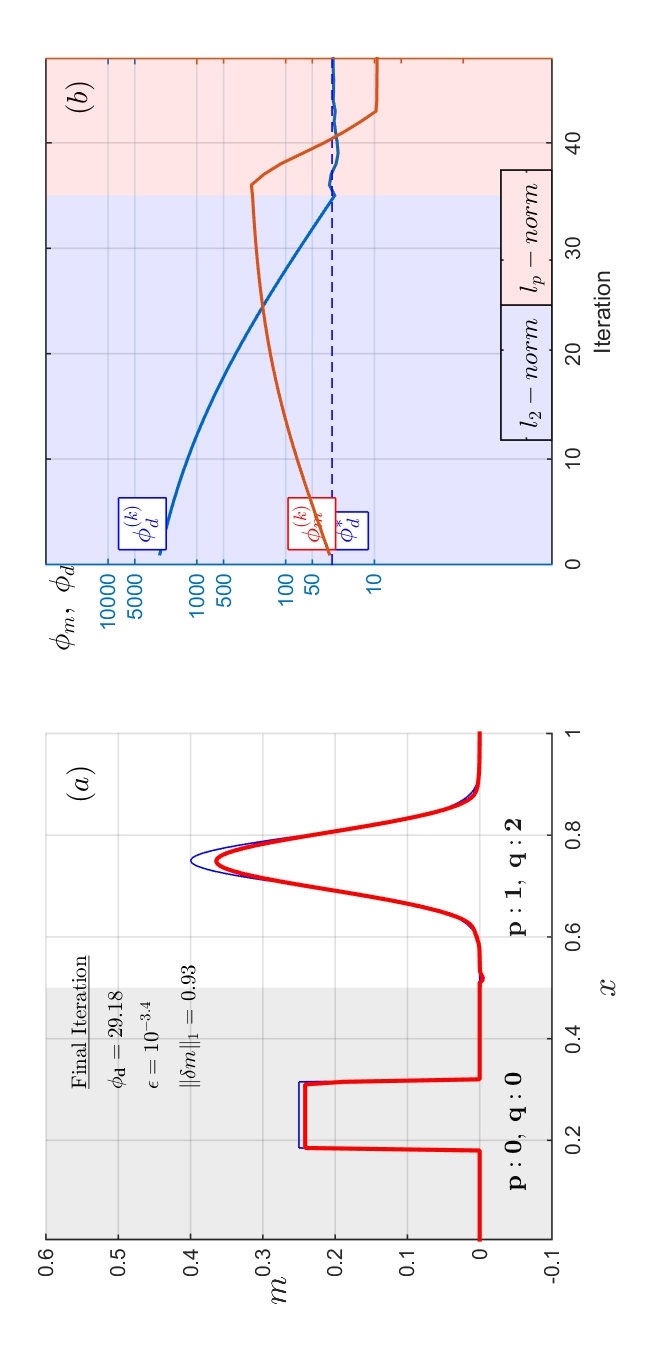
\includegraphics[scale=0.56, angle=270]{1D_Mixed_norm}
\caption{(Left) Improved solution for the 1-D problem after applying a localized mixed-norm penalty, where the regularization is divided into two regions with independent $l_p$-norm regularization: (left) $p = q = 0$, (right) $p=1 , q=2$. (Right) Convergence curves for the mixed-norm S-IRLS inversion.}
\label{fig:1D_Mixed_norm}
\end{figure}

\newpage
\subsection{2-D example}\label{2D_Section}
I test the S-IRLS algorithm on a 2-D synthetic model to further demonstrate the flexibility and robustness of the mixed-norm regularization. Analogous to the 1-D problem, the 2-D model consists of a square block and a smooth Gaussian anomaly, only this time the observations stations are located on both sides of the model domain. 
The kernel functions are exponentially decaying cosine functions of the form:
\begin{equation}
 	e^{-\omega\:r}\cdot sin(2 \pi \omega  r)\;,
\end{equation}
as shown in Figure \ref{fig:2D_Model_Kernel_data}. 

\begin{figure}[p]
\centering
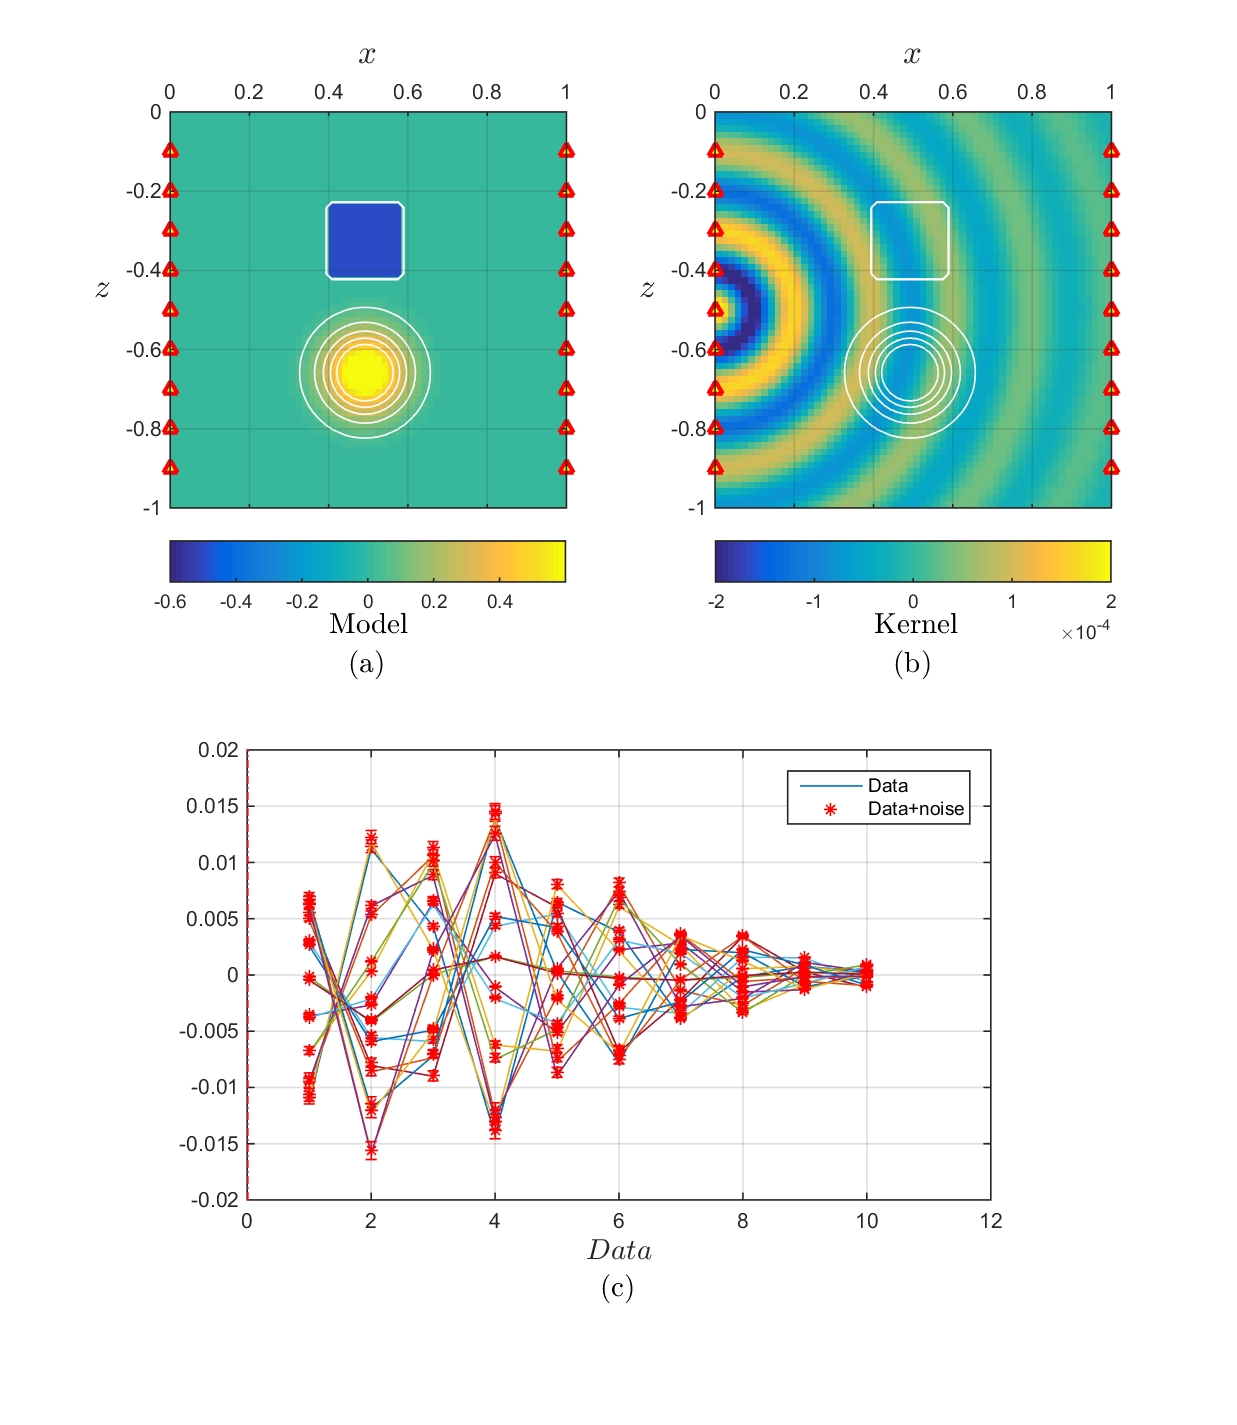
\includegraphics[scale=0.60]{2D_Model_Kernel_data}
\caption{(a) Synthetic 2-D model made up of a square block and a smooth Gaussian function. (b) Example of a kernel function for $e^{-\omega\:r}\cdot cos(2 \pi \omega  r)$ and (c) data generated from $\mathbf{d =F \; m}$. Five percent random  Gaussian noise is added. }
\label{fig:2D_Model_Kernel_data}
\end{figure}

Since we are now dealing with a 2-D problem, the regularization function involves a measure of model gradients in the $x$ and $z$-direction.
Most methods proposed in the literature, and presented in \ref{1D_Grad}, involve computing gradients with finite difference operators in orthogonal directions such that:
\begin{equation}\label{eq:grad}
\begin{split}
 	\frac{\partial m_i}{\partial x} &= \frac{m_{(i,j)} - m_{(i-1,j)}}{dx_{(i)}} \\
 	\frac{\partial m_i}{\partial z}  &= \frac{m_{(i,j)} - m_{(i,j-1)}}{dz_{(j)}}\;,
 	\end{split}
\end{equation}
where the indexes $(i,j)$ represent the cells ordering in the $x$ and $y$-direction respectively.
A second option is to penalize the absolute model gradients such that:
\begin{equation}\label{eq:mag_grad}
\begin{split}
	\nabla {m}_i  =  {\Big[ \big(\frac{\partial m_i^{(k-1)} }{\partial x}\big)^2 + \big(\frac{\partial m_i^{(k-1)} }{\partial z} \big)^2 \Big] }^{1/2}\;.
\end{split}
\end{equation}
The IRLS weights then become:
 \begin{equation}
 \begin{split}
 {\hat R}_{x_{ii}}  &= \sqrt{\tilde \eta_{q_{xi}}}{\Big[ {\left ({\nabla m_i}\right)}^{2} + \epsilon_q^2 \Big]}^{({\tilde q_{xi}}/2 - 1)/2}  \\
{\hat R}_{z_{ii}}  &= \sqrt{\tilde \eta_{q_{zi}}}{\Big[ {\left ({\nabla m_i}\right)}^{2} + \epsilon_q^2 \Big]}^{({\tilde q_{zi}}/2 - 1)/2}  \;.
   \end{split}
\end{equation}
%or
% \begin{equation}
%	\mathbf{r}_q^{(k)}  ={\Big( {(\mathbf{\nabla m}^{(k-1)})}^{2} + \epsilon^2 \Big)}^{\mathbf{q}/2 - 1} 
%\end{equation}
The same idea can easily be extended to three dimensions.
I illustrate the difference between both measures of model gradients on this 2-D problem. Figure \ref{fig:2D_Model_Grad_Test}(a) presents the recovered model using an $l_1$-norm penalty on the model gradients from the finite difference formulation. This yields blocky right-angled anomalies. Alternatively, penalizing the absolute model gradients from \eqref{eq:mag_grad}  allows for smooth corners as shown in \ref{fig:2D_Model_Grad_Test}(b). Both methods are valuable as they promote different solutions, which in some cases may better reflect the geometry of the true model. 

To accommodate both the blocky and the smooth anomaly, I divide the model space into three zones.
Figure \ref{fig:2D_Mix_lp_norms} presents the different $l_p$-norm zones defined over the two anomalies.
I extend the procedure of sub-regions presented in Section~\ref{Localized_lp} to this 2-D problem.
I impose sparse model values with the $l_1$-norm over the background region in order to get a simple model.
The norm on model gradient is variable and reflects the expected characteristics of the true model.   
I purposefully chose regions larger than the extent of the known anomalies in order to simulate a choice that could be made for a blind inversion. The goal is also to see if the transition from an $l_2$-norm to a $l_0$-norm can be done smoothly without creating artifacts.
Figure \ref{fig:2D_Mix_norm_result}(a) and (b) presents the recovered model after Phase l and Phase lll of the S-IRLS algorithm previously introduced in Table~\ref{tbl:IRLS_v4}.
Both models fit the data within 2\% of the target misfit $\phi_d^*$
The final mixed-norm model nicely recovers the blocky and smooth Gaussian anomaly. The transitions between the different $l_p$-regions appear to be seamless.

\begin{figure}[h]
\centering
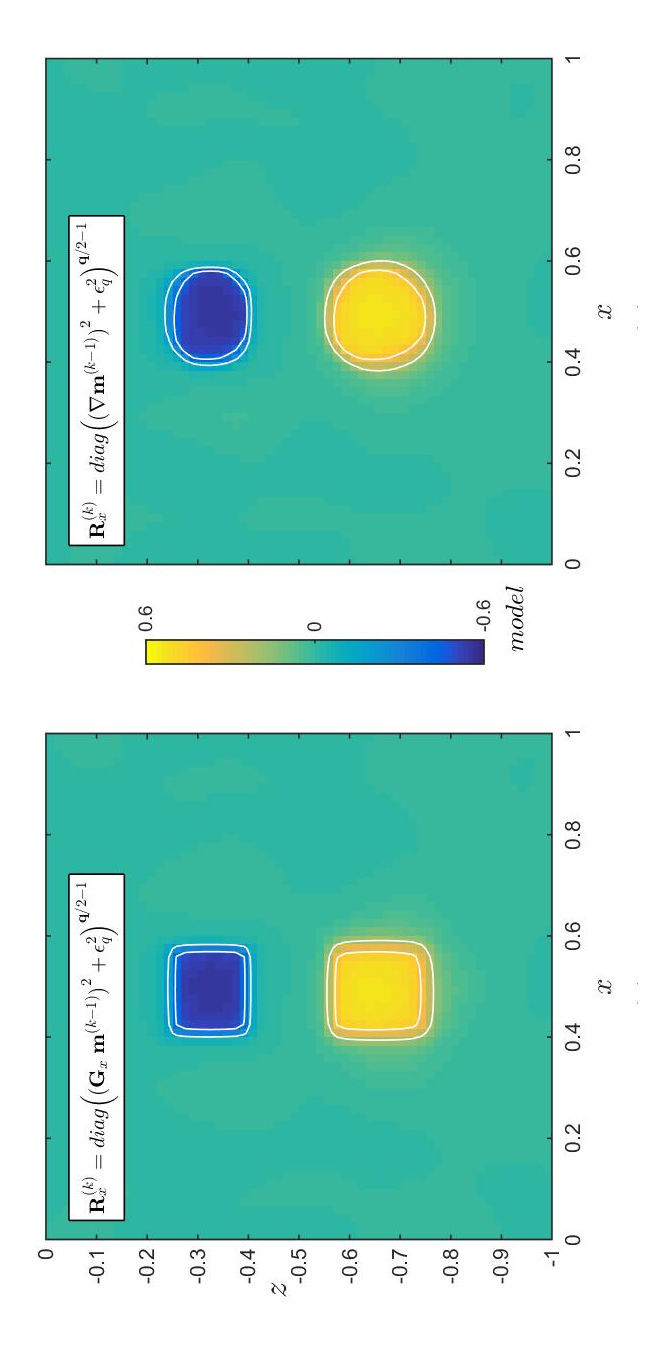
\includegraphics[scale=0.55, angle=270]{2D_Model_Grad_Test}
\caption{(a) Recovered model for $p = q_x = q_z = 1$ penalizing finite difference gradients in orthogonal directions, yielding right-angled anomalies. (b) Recovered model for the same norms but penalizing the absolute gradient of the model ($|\nabla \mathbf{m}|$) recovering round edges.}
\label{fig:2D_Model_Grad_Test}
\end{figure}

\begin{figure}[h!]
\centering
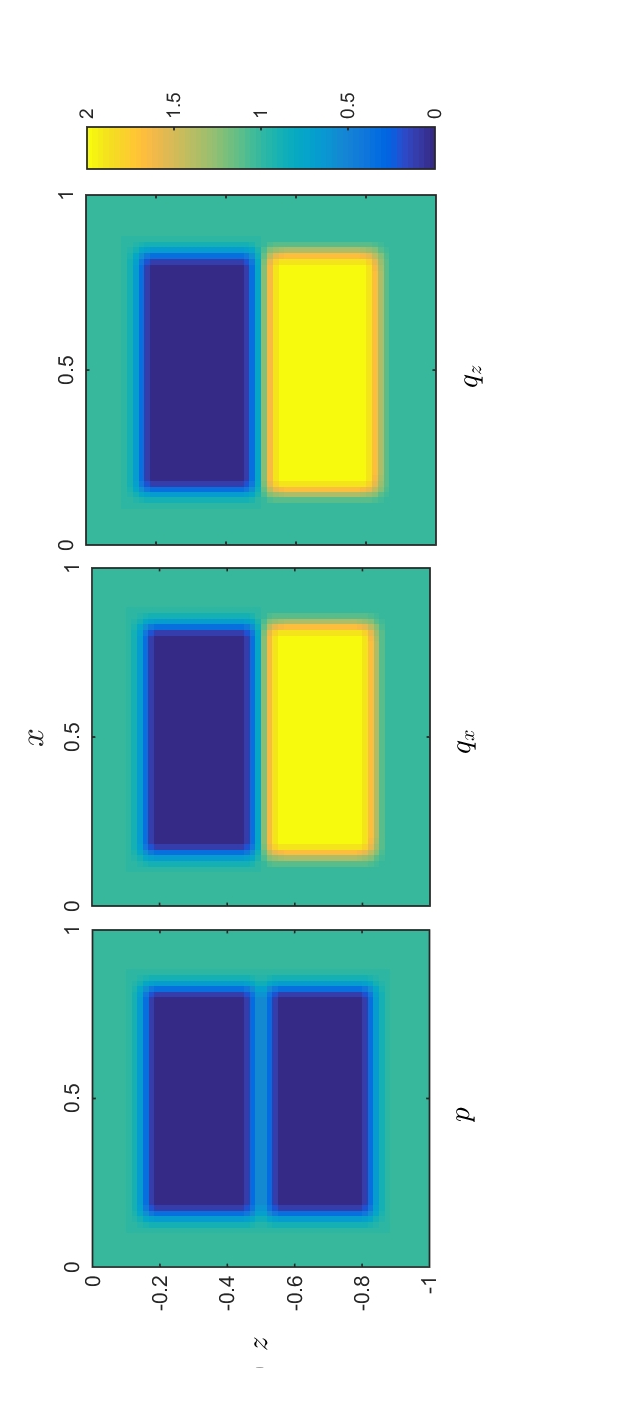
\includegraphics[scale=0.55, angle=270]{2D_Mix_lp_norms}
\caption{Distribution of $l_p$-norm on the model and model gradients over the 2-D model domain. The original boundary of each region was smoothed in order to get a slow transition and reduce visible artifacts. Regions were chosen to cover a larger area than the anomalies to simulate  a blind-inversion. }
\label{fig:2D_Mix_lp_norms}
\end{figure}

\begin{figure}[p]
\centering
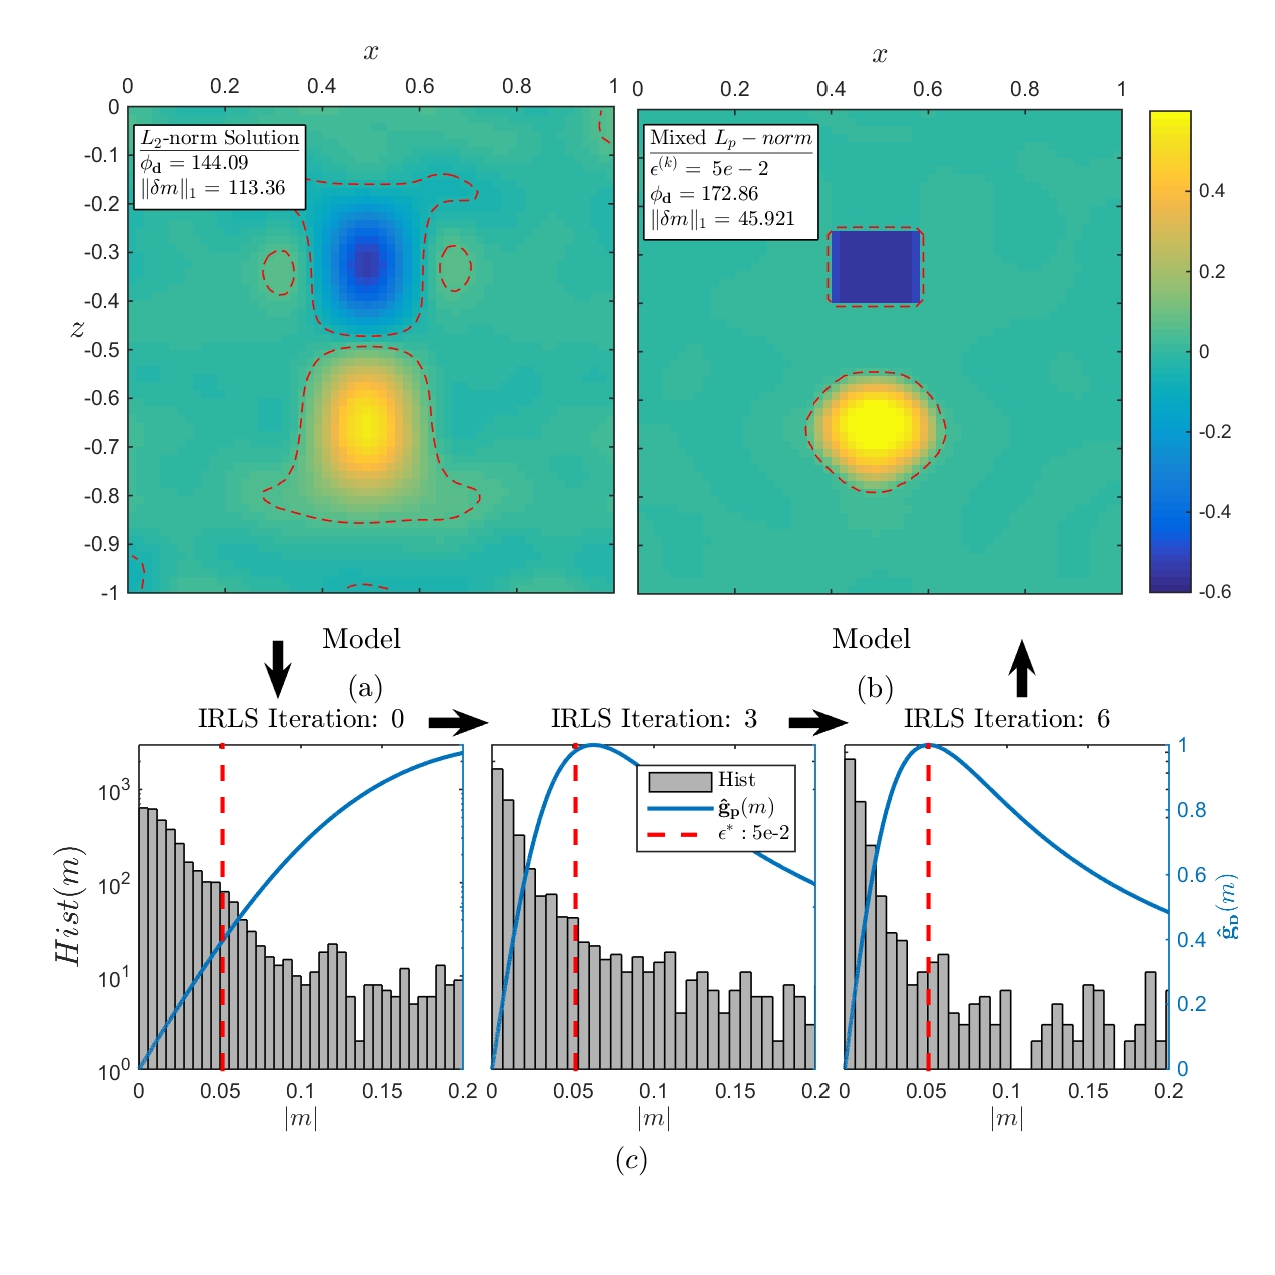
\includegraphics[scale=0.6]{2D_Mix_norm_result}
\caption{(a) Smooth $l_2$-norm solution used to initiate the IRLS iterations. (b) Recovered model using the mixed-norm regularization after seven S-IRLS iterations. The contour line (red) marks the value of $\epsilon_p$, judged to be the \emph{effective zero} value of the model ($m_i \leq $  5e-2). Both models (a) and (b) fit the data within 2\% of the target misfit $\phi_d^*$. (c) Dual plots showing the distribution of model parameters and the gradient of the $l_0$-norm penalty function $\mathbf{\hat g_p}(m)$ as a function of S-IRLS iterations. High penalties are applied to progressively smaller model values.
The final model nicely recovers both the blocky and smooth Gaussian anomaly.}
\label{fig:2D_Mix_norm_result}
\end{figure}


\newpage
\subsection{3-D example}
 As a final test, I invert the same synthetic 3-D susceptibility example as presented in Section \ref{ch:Chap3_MSI}. The model consists of a folded anomaly with magnetic susceptibility of 0.075 SI, arching around a discrete block with susceptibility of 0.05 SI. The arc-shaped anomaly is dipping $20^\circ$ towards the south. 
 
I impose sparsity constraints on the model gradients such that ($p=0,\; q_x=2,\; q_y=2,\; q_z=2$).
 Figure \ref{fig:3D_Inv_l0l2_model_INDUCED} shows the recovered model after five IRLS iterations. The solution is remarkably closer to the true solution, both in shape and model values compared to the smooth $l_2$-norm solution. The inversion also has an easier time reproducing the high frequency content from the data as shown in Figure \ref{fig:3D_Inv_l0l2_pred_INDUCED}. The inversion successfully recovers two distinct objects, no longer connected at depth. Notice that both arms are well defined and extend along the entire length of the arc.
 
As a second experiment, I impose a constraint on the model gradients in order to recover a blocky model.
Model gradients are measured with the standard finite difference operators, expected to yield right-angled anomalies.
Figures~\ref{fig:3D_Inv_l0l0_model_INDUCED} and \ref{fig:3D_Inv_l0l0_pred_INDUCED} show the recovered model and predicted data for $(p = 0,\; q = 1)$, yielding a sparse and blocky solution.
Once gain, compared to the smooth $l_2$-norm solution, the correlated data residuals are substantially reduced.
The recovered susceptibility values within the block and arc shape are more uniform than with the smoothness constraint, ideal to get a bulk estimate in physical property.
 
 \newpage
\begin{figure}[h!]
\centering
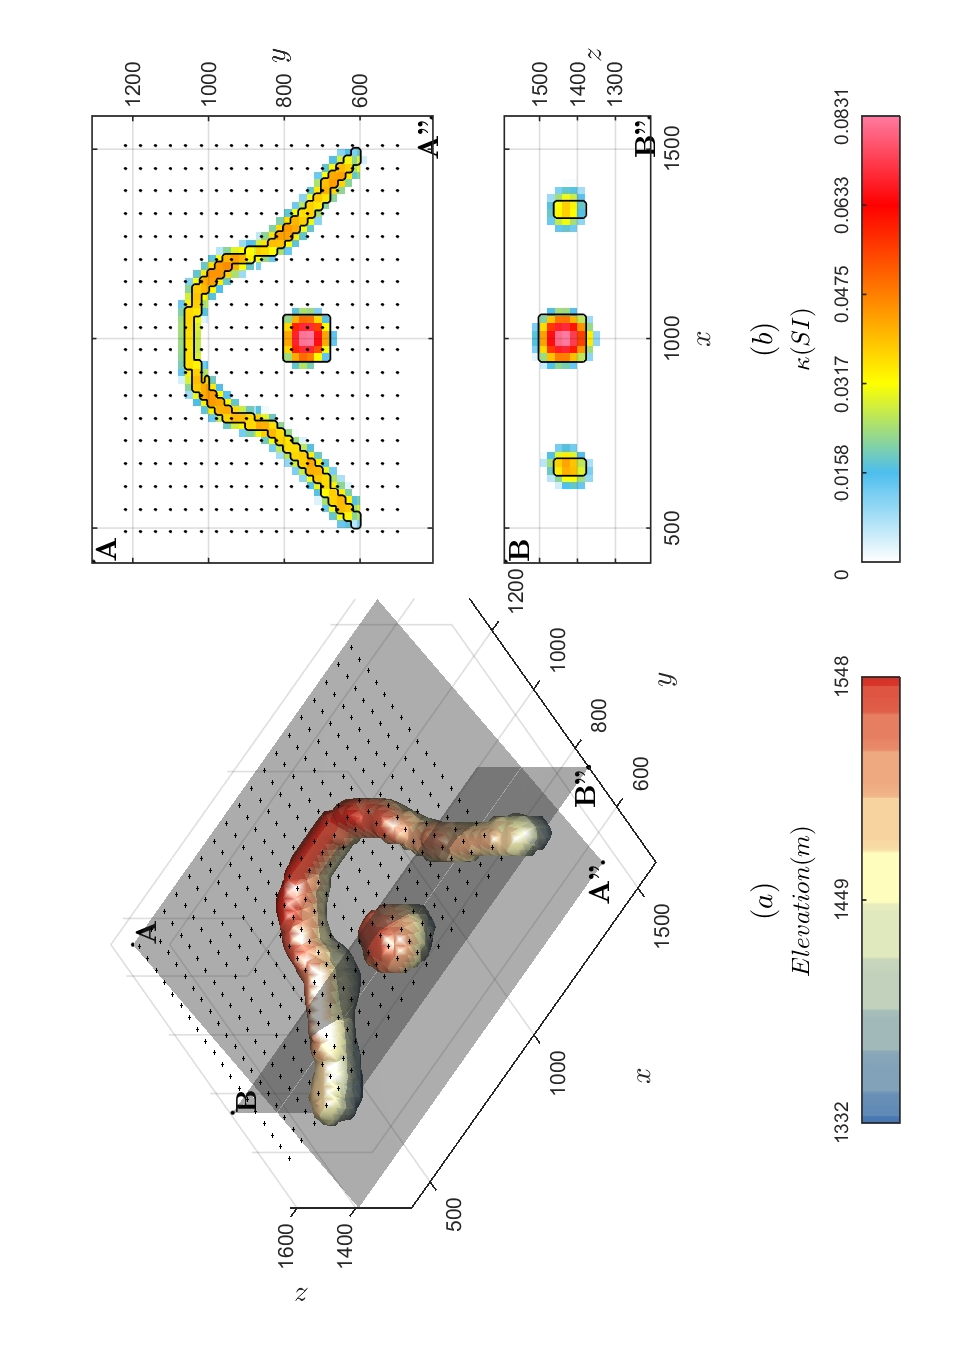
\includegraphics[scale=0.52, angle =270]{3D_Inv_l0l2_model_INDUCED.pdf}
\caption{ (a) Iso-surface (0.002 SI) and (b) sections through the recovered susceptibility model after five IRLS iterations for $(p = 0,\; q = 2)$. The final model is substantially closer to the true solution.}
\label{fig:3D_Inv_l0l2_model_INDUCED}
\end{figure}
\begin{figure}[h!]
\centering
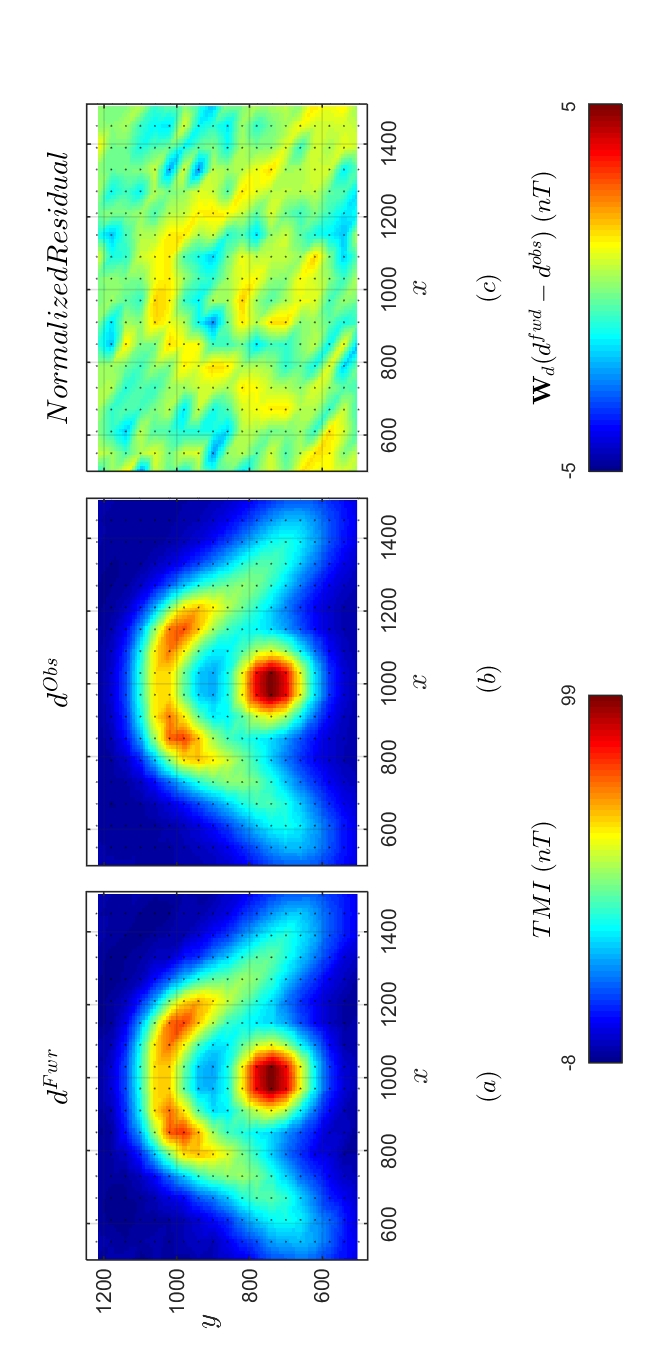
\includegraphics[scale=0.52, angle =270]{3D_Inv_l0l2_pred_INDUCED.pdf}
\caption{ Comparison between (a) observed and (b) predicted data from the recovered susceptibility model using compact norms for  $(p = 0,\; q = 2)$. (c) Normalized data residuals are within two standard deviations.}
\label{fig:3D_Inv_l0l2_pred_INDUCED}
\end{figure}

\newpage
\begin{figure}[h!]
\centering
\includegraphics[scale=0.52, angle =270]{3D_Inv_l0l0_model_INDUCED.pdf}
\caption{ (a) Iso-surface (0.002 SI) and (b) sections through the recovered susceptibility model after nine IRLS iterations for $(p = 0,\; q = 1)$ . Sparsity constraints on the model and model gradients yield a simple and blocky model.}
\label{fig:3D_Inv_l0l0_model_INDUCED}
\end{figure}
\begin{figure}[h!]
\centering
\includegraphics[scale=0.52, angle =270]{3D_Inv_l0l0_pred_INDUCED.pdf}
\caption{ Comparison between (a) observed and (b) predicted data from the recovered susceptibility model using compact norms for  $(p = 0,\; q = 1)$. (c) Normalized data residuals are within two standard deviations.}
\label{fig:3D_Inv_l0l0_pred_INDUCED}
\end{figure}

\section{Case study - Tli Kwi Cho kimberlite complex}\label{3D_Section}
As a final test, I apply the mixed-norm S-IRLS algorithm on a magnetic data from the Tli Kwi Cho (TKC) diamondiferous kimberlite complex.
The property is located in the Lac de Gras region,  approximately 350 km northeast of Yellowknife, Northwest Territories, Canada.
The TKC deposit was originally discovered by an airborne DIGHEM survey in 1992, including frequency-domain EM and magnetic data. 
Two kimberlite pipes, dubbed DO27 and DO18, were later confirmed by drilling in 1993.  
Different volcaniclastic rock units suggests that the deposit was formed over several events \cite[]{DoyleEtAl1999}. 
The pipes are intruding into older granitic rocks of the Archean Slave Province, known to have little to no magnetite content.
A magnetic susceptibility contrast between the kimberlite and the country rocks give rise to noticeable anomalies on the observed TMA data.
Strong linear features associated with the Mackenzie dyke swarms can be observed on the eastern part of the survey.
These dykes extend over the entire Lac de Gras region and generally strike $305^\circ$N \cite[]{Wilkinson2001}. 
They are known to be near vertical and are typically between 20-50 m wide. 
This geological setting is therefore ideal for implementing a mixed-norm algorithm. 
My goal is to apply \emph{soft} constraints on the model values and model gradients in order to favor specific geometry. 

Prior to the inversion, I rotate the regional dataset by $30^{\circ}$ counterclockwise to a local coordinate system in order to align the principal axis of the dykes parallel to the grid. 
The declination of the inducing field are also rotated by $30^\circ$ to preserve the geometry of the problem.
The region of interest is discretized into 25 m cube cells.
In preparation for Phase II of the S-IRLS algorithm, a smooth solution is found with the $l_2$-norm regularization as shown in Figure \ref{fig:TKC_Mag_Models}(a).
The inversion recovers two discrete bodies corresponding to the known location of DO18 and DO27.
Two linear anomalies striking north-south correspond with the Mackenzie dyke swarms. A third anomaly intersects at right-angle running $90^{\circ}$N.
As expected from the $l_2$-norm regularization, the solution is smooth and edges are not clearly defined.
Note also that the highest recovered susceptibilities are strongly correlated with the observation locations.
Dykes appear to break up between each survey line, which is clearly an inversion artifact due to changes in sensitivities. 

I want to modify the objective function in order to recover sharp and continuous edges.
In general terms, I want to enforce large gradients perpendicular to the strike of the dykes, while imposing a sparsity constraint over the kimberlite pipes.
I divide the region of interest into four sub-regions as shown in Figure \ref{fig:TKC_Mix_Norm}:
\begin{itemize}
\item{$S_1$: Sub-region covering the Mackenzie dyke swarms on the eastern edge of the survey. 
I impose an $l_0$-norm on the model gradients in the $\hat x$-direction ($q_x = 0$) to get sharp edges along the strike of the dykes, but smooth in the other directions ($q_y, q_z, p = 2$). }
\item{$S_2$: Sub-region covering the dyke running perpendicular to  the Mackenzie dyke swarms. Similar to $S_1$, I impose an $l_0$-norm on the model gradients in the $\hat y$-direction ($q_y = 0$). }
\item{$S_3$: Sub-region covering the kimberlite pipes DO27 and DO18. I impose an $l_1$-norm on the model gradients ($q_x, q_y, q_z = 1$) and an $l_0$-norm on model value ($p=0$) in order to recover blocky and sparse anomalies. }
\item{$S_4$: Background region covering the rest of the survey area. I impose an $l_2$-norm on the model gradients ($q_x, q_y, q_z = 2$) and an $l_1$-norm on model value  ($p=1$) in order to recover a smooth and sparse model. }
\end{itemize}

Figure \ref{fig:TKC_Mag_Models}(b) presents the recovered model obtained after five iterations of the S-IRLS algorithm. 
In comparison with the smooth inversion, the edges of all three dykes are better defined and extend vertically at depth. 
The inversion may suggest the presence of a fourth dyke parallel to the Mackenzie dyke swarm, on the eastern edge of the survey.
Both DO18 and DO27 are recovered as compact bodies with higher susceptibility and well defined edges compared to the smooth $l_2$-norm inversion. 
Because of the small $l_0$-norm applied to model values, most of the near surface anomalies are removed, yielding a more compact anomaly at depth.
This is also true away from the kimberlite pipe over the background region, where a simpler model is obtained.
Predicted data for the smooth $l_2$-norm model and the final S-IRLS solution are presented in Figure \ref{fig:TKC_Obs_vs_Pred}, both within $5\%$ of the target misfit.

\begin{figure}[p]
\centering
\includegraphics[scale=0.60]{TKC_Mag_Models}
\caption{(a) (Left) Horizontal section through the recovered susceptibility model at 25 m depth below topography from the smooth $l_2$-norm regularization. (Right) Iso-surface of susceptibility values around 0.002 SI.
(b) Recovered model using the mixed-norm S-IRLS algorithm. Magnetic dykes are better recovered, imaged as continuous plates and extending vertically at depth. Susceptibility values for DO-27 and DO-18 have increased, showing as compact vertical pipes.}
\label{fig:TKC_Mag_Models}
\end{figure}

\begin{figure}[p]
\centering
\includegraphics[scale=0.60]{TKC_Mix_Norm.pdf}
\caption{Horizontal section through the mixed-norm models applied to four sub-regions with smooth transition across zones.}
\label{fig:TKC_Mix_Norm}
\end{figure}

\begin{figure}[p]
\centering
\includegraphics[scale=0.60]{TKC_Obs_vs_Pred.pdf}
\caption{(a) Observed and predicted data over the TKC kimberlite complex. (b) Residuals between observed and predicted data normalized by the estimated uncertainties (10 nT). Both the smooth and mixed-norm inversions reproduce the data within four standard deviations.}
\label{fig:TKC_Obs_vs_Pred}
\end{figure}


%\newpage
\section{Summary}
In this chapter, I reviewed and experimented with several algorithms for the approximation of $l_p$-norm measures on the model and model gradients to promote sparse and blocky solutions. 
I proposed a Scaled-IRLS algorithm in order to stabilize current inversion strategies, while reducing the computational cost. 
My algorithm offers a strategy to determine an optimal value for the stabilizing parameter $\epsilon$, previously overlooked by other researchers. This robust method is further generalized, allowing for mixed-norm penalties on the model and model gradients. Scalings are applied to the individual terms of the regularization function in order to preserve their relative importance during the inverse process. 
A solution to the non-linear inverse problem is found iteratively using Gauss-Newton steps. 

Varying the combination of $l_p$-norm of the model and its gradients allows me to shape the objective function to exhibit specific characteristics. For different geological settings, there is likely a specific combination of norms that can better recover the true geometry of causative bodies. 
Preliminary results show great promise at reducing the non-uniqueness of current potential fields inversion codes.
Because my formulation is general, the algorithm can be applied to a wide range of inverse problems. 


\endinput



%\include{Chap5_Equivalent_Source}

%% The following is a directive for TeXShop to indicate the main file
%%!TEX root = Thesis_Driver.tex
\graphicspath{{./Figures/}}
\chapter{Cooperative Magnetic Inversion (CMI)}
\label{ch:Chap5_Cooperative_Mag_Inversion_CMI}

In Chapter \ref{ch:Chap3_Inverse}, I reviewed three magnetic inversion algorithms introduced in the literature. 
The magnetic susceptibility inversion is robust and computationally cheap, but it runs into limitations whenever the direction of magnetization is not parallel to the inducing field. 
The more general Magnetic Vector Inversion (MVI) can handle any orientation of magnetization by solving directly for the magnetization vector. 
This comes at the cost of increasing the number of unknowns in our large under-determined system of equations.
The $l_2$-norm regularization yields smooth solutions that are often too complex for direct geological interpretation.
Lastly, the inversion of magnetic amplitude data can provide a good estimate of the location and strength of magnetized bodies. 
The method is less sensitive to the orientation of magnetization than an inversion carried out with an assumed direction of magnetization.
The main complication for amplitude inversion is in computing amplitude data from the observed TMI, either via Fourier transform or by the equivalent-source. The inverse problem is also non-linear with respect to the model, which increases the computational cost and is less stable. 

While all of the above inversion methods have strength and weaknesses, they each bring complementary information.
The susceptibility inversion can be used to rapidly compute an equivalent-source layer and to generate amplitude data.
The amplitude data can then be fed into the amplitude inversion to locate magnetic anomalies.
In turn, imposing a geometric constraint on the MVI can greatly reduce the non-uniqueness of the problem. 
All three algorithms share variations of the same system of equations. This is beneficial as calcuations for the sensitivity matrix can be stored and repurposed at each step.

In this chapter, I introduce a Cooperative Magnetic Inversion (CMI) method, which combines the equivalent-source, amplitude inversion and MVI method into a single inversion algorithm. 
Using the S-IRLS method from Chapter~\ref{ch:Chap4_Mixed_Lpnorm_Regularization}, I impose a sparsity constraint on the model and model gradients to further reduce the solution space.
From an imaging stand point, compact and well defined magnetic anomalies can simplify the geological interpretation.
From a practical aspect, having an algorithm that can manage all three codes reduces the number of manual steps that were previously required from the user. 

\section{Methodology}
In Chapter \ref{ch:Chap3_Inverse}, I inverted a synthetic model with complicated magnetization orientations. 
The model recovered from the MVI inversion was smooth with poor recovery of the arc anomaly (Fig.~\ref{fig:3D_Inv_l2l2_model_TMVI}).
Using the CMI algorithm, I re-invert the synthetic example using an $l_2$-norm regularization. 
I will here breakdown each step of the CMI algorithm, but I want to emphasize that the entire process is automated and can all be done as a single workflow.
I divide the algorithm in three parts as shown in Figure \ref{fig:Advanced_Mag_Inversion_Algo} in schematic form.

 \begin{figure}[h!]
\centering
\includegraphics[scale=0.6]{Advanced_Mag_Inversion_Algo.png}
\caption{ Schematic representation of the Cooperative Magnetic Inversion (CMI) algorithm. Input and output parameters are indicated by a dash arrow.}
\label{fig:Advanced_Mag_Inversion_Algo}
\end{figure}

Stage I of the algorithm is mainly a data preparation step, ahead of the amplitude inversion and MVI.
As in other inversion methods, the algorithm requires TMA data and a mesh.
The algorithm computes the large system of equations needed for sensitivity calculations as defined by \ref{Tensor_T}.
Following the sensitivity calculations, the algorithm proceeds with an equivalent-source layer inversion as described in Section\ref{EQS}.
Figure~\ref{fig:3D_EQS_CMI} presents the inverted effective susceptibility layer and predicted data at the station locations.
Amplitude data are saved and passed on to Stage II.
\begin{figure}[p]
\centering
\includegraphics[scale=0.55]{3D_EQS_CMI.pdf}
\caption{ (a) Inverted equivalent-source layer and (b-f) predicted $\hat x$, $\hat y$, $\hat z$-component, TMI and magnetic amplitude data for the synthetic model.}
\label{fig:3D_EQS_CMI}
\end{figure}

In Stage II, the algorithm proceeds with the amplitude inversion from Section~\ref{MAI}.
Figure~\ref{fig:3D_Inv_l2l2_CMI_kEff} shows the recovered smooth effective susceptibility model.
The recovered effective susceptibility model is then converted to sensitivity weighting matrix such that:
\begin{equation}\label{W_M}
{W}_{m_{ii}} =  {\Big[\frac{\kappa_{e_i} *0.9 }{max(\kappa_{e})} + 0.01\Big]}^{-1}  \;,
\end{equation} 
 where $\mathbf{W}_m \in \mathbb{R}^{nc \times nc}$ is a diagonal matrix of the normalized effective susceptibilities $\kappa_{e}$. A small number (1e-2) is added to assure that all values are between [1 100].
 This type of re-scaling was determined empirically to be robust. 
The sensitivity weighting matrix is saved and passed on to the MVI inversion.

\begin{figure}[h!]
\centering
\includegraphics[scale=0.52, angle =270]{3D_Inv_l2l2_model_kEff.pdf}
\caption{ (a) Iso-surface (0.002 SI) and (b) sections through the recovered effective susceptibility model. This effective susceptibility model is used to construct a weighting matrix to constrain the MVI.}
\label{fig:3D_Inv_l2l2_CMI_kEff}
\end{figure}
\begin{figure}[h!]
\centering
\includegraphics[scale=0.52, angle =270]{3D_Inv_l2l2_pred_kEff.pdf}
\caption{Comparison between (a) observed and (b) predicted data from the recovered effective susceptibility model. The inversion can predict most of the data within one standard deviation.}
\label{fig:3D_Inv_l2l2_pred_kEff}
\end{figure}

In Stage III, the regularization function is pre-multiplied by the effective susceptibility weighting calculated in \ref{W_M}.
The model objective function becomes:
\begin{equation} \label{eq:S-IRLS_CMI}
\begin{aligned}
\phi(m) =  \phi_d + \beta \gamma^{(k)} \Big [ {\|\mathbf{W}_m\; \mathbf{W}_s\;  \mathbf{\hat R}_s \;( \mathbf{m - m^{ref}})\|}^2_2  + \sum_{i = x,y,z}  {\| \mathbf{W}_m\;  \mathbf{W}_i \;  \mathbf{\hat R}_i  \; \mathbf{G}_i \; \mathbf{m}\|}^2_2  \Big ]\;.
\end{aligned}
  \end{equation}
 The model weighting matrix $\mathbf{W}_m$ imposes a high penalty on cells that received low effective susceptibility from the amplitude inversion. 
 Figure \ref{fig:3D_Inv_l2l2_model_AMI} presents the inverted model after reaching the target data misfit. The added information from the amplitude inversion greatly improves the solution over the MVI alone. Although still smoothly varying, the inversion manages to separate the arc and the block anomaly, while also recovering the orientation of magnetization.

\newpage
 \begin{figure}[h!]
\centering
\includegraphics[scale=0.52, angle =270]{3D_Inv_l2l2_model_AMI.pdf}
\caption{ (a) Iso-surface (0.005 SI) and (b) sections through the recovered magnetization model from the CMI algorithm $(p = 2,\; q = 2)$ . The inversion recovers both the arc and the block anomaly as distinct objects.}
\label{fig:3D_Inv_l2l2_model_AMI}
\end{figure}
\begin{figure}[h!]
\centering
\includegraphics[scale=0.52, angle =270]{3D_Inv_l2l2_pred_AMI.pdf}
\caption{ Comparison between (a) observed and (b) predicted data from the recovered susceptibility model. (c) Normalized data residuals are within two standard deviations.}
\label{fig:3D_Inv_l2l2_pred_AMI}
\end{figure}

\newpage
\section{CMI with S-IRLS regularization}
As a final experiment I impose sparsity constraints on the amplitude inversion for $(p = 0,\; q = 1)$, in order to simplify the distribution of effective susceptibility. 
The goal is to get a simpler effective susceptibility model to further reduce the active space of the MVI algorithm. It is a $soft$ constraint on the solution as I do not impose $a\;priori$ information to individual cells, but rather a general constraint on the behavior of the solution. Figure~\ref{fig:3D_Inv_l0l1_CMI_kEff} presents the recovered model after convergence.

 The $l_p$-norm constraint considerably reduces the complexity of the model, although some artifacts remain at depth from the amplitude inversion.
 In Stage III, the compact effective susceptibility model is used to constrain the MVI result.
 Figure~\ref{fig:3D_Inv_l0l1_model_AMI} presents the final magnetization vector.
 The arc and the central block are recovered at the right location and effective susceptibility values are near the true model. 
 From a mineral exploration perspective, the model showed in \ref{fig:3D_Inv_l0l1_model_AMI}  would be easily interpreted.
 I note that most of the deep artifacts from the amplitude inversion have been removed. The final data residual is within one standard deviation, and no longer shows structure correlated with the magnetic anomaly.

\begin{figure}[h!]
\centering
\includegraphics[scale=0.52, angle =270]{3D_Inv_l0l1_CMI_kEff.pdf}
\caption{ (a) Iso-surface (0.01 SI) and (b) sections through the recovered effective susceptibility model from the amplitude inversion with sparsity constraint applied $(p = 0,\; q = 1)$. The $l_p$-norm constraint considerably reduces the complexity of the model, although the model is still stretched vertically.}
\label{fig:3D_Inv_l0l1_CMI_kEff}
\end{figure}
\begin{figure}[h!]
\centering
\includegraphics[scale=0.52, angle =270]{3D_Inv_l0l1_CMI_pred_kEff.pdf}
\caption{Comparison between (a) observed and (b) predicted amplitude data from the recovered compact effective susceptibility model $(p = 0,\; q = 1)$. (c) Normalized data residuals are within two standard deviations.}
\label{fig:3D_Inv_l0l1_CMI_pred_kEff}
\end{figure}

\begin{figure}[h!]
\centering
\includegraphics[scale=0.52, angle =270]{3D_Inv_l0l1_model_AMI.pdf}
\caption{ (a) Iso-surface (0.01 SI) and (b) sections through the recovered magnetization model from the CMI algorithm. Compact norms $(p = 0,\; q = 2)$ were applied during the amplitude inversion. The $l_p$-norm constraint considerably reduces the complexity of the model.}
\label{fig:3D_Inv_l0l1_model_AMI}
\end{figure}
\begin{figure}[h!]
\centering
\includegraphics[scale=0.52, angle =270]{3D_Inv_l0l1_pred_AMI.pdf}
\caption{ Comparison between (a) observed and (b) predicted data from the recovered magnetization CMI model. (c) Normalized data residuals are within two standard deviations. Correlated residuals are no longer seen.}
\label{fig:3D_Inv_l2l2_pred_AMI}
\end{figure}

 \section{Conclusion}   
In this chapter, I implemented a Cooperative Magnetic Inversion for the inversion of magnetization vectors.
The algorithm ties together three inversion algorithms previously introduced in the literature: the magnetic susceptibility, magnetic amplitude and MVI.
The recovered vector magnetization models are simpler and more representative of the true solution. 
The inversion process is automated, hence reducing the overall work required, both numerically and from the end-user. 
    


\endinput



%% The following is a directive for TeXShop to indicate the main file
%%!TEX root = Thesis_Driver.tex
\graphicspath{{./Figures/}}
\chapter{Case Study}
\label{ch:Chap6_Case_Study}

In this chapter, I apply the CMI algorithm on a 1992 aeromagnetic data set collected over the Ekati Property, Northwest Territories.
Airborne magnetic surveys have been an integral part of diamond exploration in the region since the early 1990s \cite[]{Pell1997}.
The Lac de Gras region has been particularly productive, hosting two of the largest deposits found in Canada, the Ekati and Diavik mines.
Over 150 kimberlites have been identified on the Ekati Property \cite[]{Carlson2015}, but diamond grades are highly variable.
It is estimated that less than 10$\%$ of the 150 known kimberlites on the Ekati Property are of economic interest.
While most kimberlite pipes can easily be identified by their geophysical signature, estimating the economic potential early in the exploration stage remains challenging \cite[]{CoopersmithEtAl2006}.

Kimberlite pipes are generally magnetic anomalies known to retain a strong remanent component.
There have been several studies specifically dedicated to magnetic methods applied to kimberlite deposits.
Previous geophysical studies relied primarily on data processing techniques to isolate exploration targets \cite[]{Cowan2000}.
Direct inversion of magnetic data over remanently magnetized kimberlite pipes has long been challenging for reasons discussed in Chapter \ref{ch:Chap3_Inverse}.
In \cite{Shearer05}, the magnetic amplitude inversion is implemented on a data set from the Galaxie trend, Nunavut.
The location and geometry of negative magnetic anomalies were successfully inverted and attributed to hypabyssal kimberlite dykes, later confirmed by drilling.
A few years later, \cite{Zhao2012} inverted a subset of a large-scale aeromagnetic survey over the Ekati Property.
The inclination and amplitude of magnetization were computed for the Grizzly and Leslie pipes and compared to the 2D analysis done by \cite{Cheman2006}.

In this chapter, I invert the large data set that was partially analyzed by \cite{Zhao2012}, over the Ekati Property.
Using the CMI algorithm introduced in Chapter \ref{ch:Chap5_Cooperative_Mag_Inversion_CMI}, I extract regional information about the distribution of dyke swarms in relation to the known kimberlite deposits.
I then proceed with deposit-scale inversions over 17 of the known pipes and recover a bulk estimate of the magnetization. The recovered orientations of magnetization are compared to physical property measurements from the literature.
Finally, I compare the published radiometric dating on 11 of those pipes with the polarity predicted from the inversion and the global geomagnetic timescale. 


\section{Ekati Property}
The Ekati Property is located north of the Lac de Gras region, approximately 300 km northeast of Yellowknife, Northwest Territories.
The current mineral claim covers an area of over 262,000 ha.
Since discovery of the first kimberlite in 1991, over 150 additional pipes were identified from geophysical surveys, till sampling and drilling programs.
Figure \ref{fig:Ekati_Location} shows the topography and locations of known pipes over the region.
The Panda and Beartooth pipes were actively mined between the period of 1998 and 2010 and are now fully depleted.
Three are still under production: Misery, Koala and Koala North.
Since the beginning of operations in 1999, over 58 million carats have been extracted from the various kimberlite pipes \cite[]{Carlson2015}.
South of Ekati is the Diavik mine, which has also produced over 91 million carats between 2003 and 2014 \cite[]{Yip2015}.

\begin{figure}[h!]
\includegraphics[scale=0.6]{Ekati_Location.png}
\caption{Topography and known kimberlites over the Lac de Gras region. The location of the main operations for the Ekati and Diavik mines are shown (red dot).}
\label{fig:Ekati_Location}
\end{figure}

\subsection{Geology}
The Lac de Gras kimberlite field is located in the Slave craton,  which consists mainly of granitoid and meta-sediment rocks dated between 2.66-2.58 Ga-old \cite[]{Creaser2004}.
The region is intruded by several phases of diabase dyke swarms clearly visible on the airborne magnetic data.
Table \ref{tbl:Dykes} summarizes the age and trend of five important groups of dykes \cite[]{Buchan09}.
It has been argued that the dykes may serve as structural control for kimberlites \cite[]{Wright1999}.


\begin{table}
\centering
\caption{Dyke swarms of the Lac de Gras region listed in increasing age as published by \cite{Buchan09}}
\label{tbl:Dykes}
\renewcommand{\arraystretch}{1.2}
\begin{tabular}{|c|c|c|}
Name & Orientation ($^\circ$) & Age (Ma) \\
Mackenzie & 315 & 1267 \\
$'305'$ & 305 & - \\
Lac de Gras & 0 & 2027-2023 \\
MacKay & 90 & 2210 \\
Malley & 45 & 2230
\end{tabular}
\end{table}


Kimberlite pipes in the Lac de Gras region are narrow, steeply sided inverted cones, with the majority of them covering less than 5 ha at the surface.
The standard model for kimberlites in the Lac de Gras region is a mix of fragmented crater facies and non-fragmented hypabyssal (HK) facies.
The crater facies in the upper portion of the type can be further subdivided in various types of volcaniclastic (VK) and pyroclastic (PK) units \cite[]{Pell1997}.
Found at greater depths, the HK unit is a coherent olivine-rich rock, and is also found as intrusive dykes and sills.
The composition and physical properties of kimberlites can vary greatly between pipes.
Geophysically, it has been found that crater facies are generally associated with density and magnetic susceptibility lows.
Weathering of the crater facies may also appear as resistivity lows due to the abundance of clay minerals, although they can easily be confounded with fine grained glaciofluvial sediments in northern regions \cite[]{PowerHildes2007}.
The hypabyssal facies on the other hand are mostly associated with magnetic susceptibility highs and are prone to retaining remanent magnetization.

Fossil bearing xenoliths in some pipes are indicative of a sub-marine emplacement between the Late Cretaceous to Eocene time.
Radiometric dating of 36 pipes indicates a wide range of emplacement times \cite[]{Creaser2004}, divided into five temporally discrete episodes \cite[]{Lockhart2004}. Three of the most productive kimberlites at Ekati (Koala, Koala North and Panda pipes) were emplaced 53 Ma ago during the Panda Age Array (PAA).
Physical property measurements of the rocks were also acquired over the Lac de Gras region and are summarized in \cite[]{Enkin2003, Buchan09}.
It has been suggested that the orientation of magnetization could be used to determine the age of a kimberlite pipe, hence it could be used to estimate the economic potential of a deposit \cite[]{Lockhart2004}.

\subsection{Airborne magnetic data}
In 1993, a fixed-wing magnetic survey was flown over the Ekati Property as shown in Figure \ref{fig:Aeromag_Location}.
The $''Paul's\;Lake''$ aeromagnetic data were downloaded from the Natural Resources Canada's website.
The data set consists of 91 survey lines of Total Magnetic Field (TMI) measurements, spaced 250 m apart, covering an area of $23\times36$ km.
Observations were provided at a 50 m spacing along line, at an average flight height of 120 m, as measured by radar altimeter.
From historical geomagnetic data, the inducing field strength was 60,275 nT, [I: $27^{\circ}$, D: $84^{\circ}$].

A Digital Elevation Model (DEM) was downloaded from the Canadian Digital Elevation Data collection (1:50,000), also provided by Natural Resources Canada.
The DEM was used to convert the radar height to absolute elevation referenced to mean sea level.

\begin{figure}[h!]
\includegraphics[scale=0.6]{Aeromag_Location.png}
\caption{Topography, aeromagnetic survey and known kimberlites over the Lac de Gras region. The location of the main operations for the Ekati and Diavik mines is marked with a red dot.}
\label{fig:Aeromag_Location}
\end{figure}


\section{Regional scale inversion}
The inversion procedure follows the methodology presented in Chapter \ref{ch:Chap5_Cooperative_Mag_Inversion_CMI}.
The objective of a regional scale inversion is to first gain knowledge about the general distribution of magnetic anomalies.
Moreover, this step is used to estimate uncertainties and to identify regions of interest for a deposit-scale inversion.

Prior to the inversion, I remove a regional trend in the data in order to focus the inversion on local anomalies. Small regions 1 $km^2$ showing low variations in the field were manually chosen as shown in Figure~\ref{fig:Ekati_Detrend_Data}(a). Within each region, the median data value and horizontal location are recorded. Those values are then used to create a first-order polynomial (Fig-\ref{fig:Ekati_Detrend_Data}(b)). A regional trend of roughly 250 nT trending up towards east is subtracted as shown in Figure~\ref{fig:Ekati_Detrend_Data}(c). I assign five percent uncertainties, plus 5 nT floor uncertainty to the data.   

\begin{figure}[h!]
\centering
\includegraphics[scale=0.55, trim= 1cm 0 0 0]{Ekati_Detrend_Data.png}
\caption{Regional data (a) before and (c) after removal of a regional trend. The median value within selected regions (boxes) were used to compute (b) a first-order polynomial trend.}
\label{fig:Ekati_Detrend_Data}
\end{figure}

Table \ref{tbl:Reg_inv} presents some of the parameters used for the inversion.
The model space is discretized by a 50 m cell size resolution.
The depth extent of the mesh covers the top 1 km below topography,  for a base mesh of 6 M cells.
Inversion of the entire data set, approximately 50,000 observations, at this resolution remains computationally challenging for most computers.
In order to reduce the computational cost, I designed a tiled inversion procedure. Figure \ref{fig:Ekati_Tiles} presents the tiling configuration with respect to the data set.
Neighboring regions overlap by 500 m in order to share a minimum of two survey lines, guaranteeing good lateral continuity.
The procedure is readily parallelized across multiple processors, each inverting a subset of the problem independently.
The final magnetization model is interpolated onto the base mesh using a weighted average scheme such that:

\begin{equation}\label{merge}
\begin{split}
m_i &= \frac{\sum_{j=t}^T m_i^{(j)} \; w_i^{(j)}}{\sum_{j=t}^T w_i^{(j)}} \\
w_i^{(j)} & = {\Big[ { (x_i - x_c^{(j)})}^2 + { (y_i - y_c^{(j)})}^2 \Big]}^{-1/2} \;,
\end{split}
\end{equation}
where the weights $w_i^{(j)}$ are inverse distance between the $i^{th}$ cell and the center location $[x_c;y_c]$ of the $j^{th}$ tile. The number of tiles T overlapping at the $i^{th}$ cell is variable depending on the horizontal location. The same weight is used for all cells vertically at the same $[x_i;y_i]$ location.

\begin{figure}[h!]
\centering
\includegraphics[scale=0.38]{Ekati_Tiles.png}
\caption{TMA data after removal of the regional signal and tiling configuration used for the regional inversion.}
\label{fig:Ekati_Tiles}
\end{figure}

\begin{table}
\centering
\caption{Regional-scale inversion parameters.}
\label{tbl:Reg_inv}
\renewcommand{\arraystretch}{1.2}
\begin{tabular}{|c|c|}
Core cell size & $75\times75\times50$ m \\
Base mesh size & 3.3 M cells \\
Number of tiles & 77 \\
M / tile & $\approx$ 100k cells \\
N / tile & $\approx$ 900 data \\
$p,\;qx,\;qy,\;qz$ & 1, 1, 1, 1 \\
$\alpha_s,\; \alpha_x,\; \alpha_y, \; \alpha_z$ & 1.8e-4, 1, 1, 1 \\
Uncertainties & 0.05*d + 5 nT
\end{tabular}
\end{table}

Figure \ref{fig:Ekati_Reg_Interp} presents a horizontal section at $\approx$50 m depth through the recovered effective susceptibility model.
As expected from the observed data, several long and narrow anomalies are recovered.
Based on the analysis by \cite{Buchan09}, I interpret the linear trends as regional dyke swarms belonging to the Mackenzie, Lac de Gras, MacKay and Malley groups.
A large number of kimberlite pipes show as effective susceptibility highs, with few exceptions.
The three Koala pipes, for example, west of the Grizzly pipe, were not well recovered.
Although important economically, the anomalous magnetic response from the pipe is below the noise level.
Proper imaging of the deposits would require a magnetic survey at lower elevation to increase the noise to signal ratio.

I note the clustering of kimberlite pipes near the intersection and along some of the dyke swarms.
The apparent correlation between kimberlite pipes and dykes seems to reinforce the idea of structural controls as put forward by \cite{Wright1999}.
While the topic is beyond the scope of this Masters thesis, future work in structural geology over the region may benefit from a regional scale inversion as presented here.

Figure~\ref{fig:Ekati_reg_Obs_Pred} compares the observed and predicted data from the tiled inversion. In the left panel, the predicted data from individual tiles were merged following \ref{merge}. The normalized residual data show horizontal striations due to variations in magnetic data between adjacent lines, which could not be accounted for by the inversion. 
Overall, each invividual inversion could predict the data well within the assigned uncertainties.
On the other hand, the right panel shows the predicted data from the final merged susceptibility model.
I here notice that some of the low frequency content has been lost during the merging process, with higher residuals over the regions of low magnetic fields.
This can be a problem when attempting to image regional features and will require further research.
In this case, we are only interested in the dykes and kimberlite pipes, which for the most part were well recovered.

\begin{figure}[h!]
\centering
\includegraphics[scale=0.58, trim= 0.5cm 0 0 0]{Ekati_Reg_geology_interp.png}
\caption{Interpreted dykes (line) from the property-scale magnetization inversion and known kimberlite pipes location (circle). The 16 pipes chosen for a deposit-scale inversion are labeled.}
\label{fig:Ekati_Reg_Interp}
\end{figure}

\begin{figure}[h!]
\centering
\includegraphics[scale=0.6, trim=0.75cm 0 0 0]{Ekati_reg_Obs_Pred}
\caption{Comparison between (a) observed and (b) merged predicted data from the recovered magnetization model over the Ekati Property. (c) Normalized residual data show horizontal striations due to variations in magnetic data between adjacent lines, which could not be accounted for by the inversion. Most of the predicted data from the individual tiles can fit the observed data within one standard deviation. (d) Forward modeled data from the merged magnetization model and (c) normalized data residual. It appears that a large portion of the the low frequency content has been lost during the merging step. More research is required in order to preserve the long wavelength information.}
\label{fig:Ekati_reg_Obs_Pred}
\end{figure}

\section{Deposit scale inversion}
From the property scale inversion, 16 sites were chosen based on the strength of the magnetic anomaly for a high resolution inversion.
The goal of this section is to gain knowledge about the bulk magnetization direction and compare those values to physical property measurements published in the literature.

For each inversion, a regional field was removed in order to focus the inversion on the local anomalies.
Description of the regional field removal method can be found in \cite{LiRegRem1998}.
In summary, the following steps were taken:
\begin{itemize}
\item Creation of a local mesh with large padding cells
\item Inversion of the data assuming induced magnetization
\item Removal of the local source within the core mesh. Only susceptible material outside the core region remain.
\item Forward modeling of the regional data at the observation location
\item Subtraction of the regional signal from the observed data
\end{itemize}
The regional-removal step is important in regions where the regional field is larger than the local anomaly.
Figure \ref{fig:RegRem_Misery} presents the magnetic data before and after removal of the regional field over the Misery pipe.
Note that the original data are trending up towards the east, with the largest magnetic field data occurring near the edge of the dataset. Consequently, the magnetic amplitude inversion would be biased towards having a ring of effective susceptibility around the edge of the dataset, rather than the pipe itself. 
After removing the regional field, most of the anomalous fields come from a strong negative anomaly corresponding with the location of the Misery pipe.

\begin{figure}[h]
\centering
\includegraphics[scale=0.55,angle=270]{RegRem_Misery}
\caption{(a) Local data collected over the Misery pipe showing a local western trend. (b) Regional field data are computed from a local inversion. Most of the signal comes from a dyke running north-south along the western edge of the local tile. (c) Residual data after regional field removal, showing a clear reversely magnetized anomalie corresponding with the location of the Misery pipe.}
\label{fig:RegRem_Misery}
\end{figure}

Following the regional field removal, each local tile is inverted with the CMI algorithm on a 25 m cell size mesh.
This resolution is required in order to properly model narrow anomalies in the range of 50 to 100 m in width.
The process was repeated for the selected 16 kimberlite pipes.
Table \ref{tbl:Dep_inv} summarizes the parameters used for the inversions.
I imposed an $l_0$-norm on the amplitude of magnetization in order to focus the inversion within the core of the different kimberlites pipes. The direction of magnetization was allowed to vary smoothly in order to get an estimate of the variability, and hence to get a measure of uncertainty. A 27 point average (3x3x3 cells) centered over the location of each pipe was used to compute an effective susceptibility and direction as shown in Table \ref{Local_Summary}.
In the following section, the results are compared to those published in the literature.


\begin{table}
\centering
\caption{Deposit-scale inversion parameters.}
\label{tbl:Dep_inv}
\renewcommand{\arraystretch}{1.2}
\begin{tabular}{|c|c|}\hline
Core cell size & $25\times25\times25$ m \\
Base mesh size & 50 M cells \\
Number of tiles & 17 \\
M / tile & $\approx$ 200k cells \\
N / tile & $\approx$ 150 data \\
$p,\;qx,\;qy,\;qz$ & 0, 2, 2, 2 \\
$\alpha_s,\; \alpha_x,\; \alpha_y, \; \alpha_z$ & 1.6e-3, 1, 1, 1 \\
Uncertainties & 0.02*d + 5 nT \\ \hline
\end{tabular}
\end{table}
\begin{table}[]
\centering
\caption{Average magnetization amplitude and direction from the local inversion over 16 known kimberlite pipes. Uncertainties were calculated from a three-cell cube standard deviation around the approximate location of each kimberlite pipe.}
\label{Local_Summary}
\renewcommand{\arraystretch}{1.}
\begin{tabular}{|c|c|c|c|c|c|}\hline
Pipe ID &	X (m) &	Y (m) &	$\kappa_{e}$ &	Incl ($^{\circ}$) &	Decl ($^{\circ}$) \\ \hline
Arnie &	532980 &	7176930 &	3.9e-2 $\pm$ 1.0e-2 &	 -85 $\pm$ 4.2 &	 355 $\pm$ 5.0 \\
Blackbear &	519700 &	7176980 &	9.9e-4 $\pm$ 1.3e-4 &	 -88 $\pm$ 1.9 &	 211 $\pm$ 3.0 \\
Brent &	530855 &	7174206 &	4.6e-3 $\pm$ 2.0e-3 &	 -79 $\pm$ 3.1 &	 299 $\pm$ 2.3 \\
Fox &	515091 &	7169946 &	2.4e-2 $\pm$ 8.0e-3 &	 66 $\pm$ 17.7 &	 203 $\pm$14.9 \\
Grizzly &	521529 &	7177946 &	8.7e-2 $\pm$ 8.6e-3 &	 -82 $\pm$ 1.3 &	 100 $\pm$ 1.7 \\
Hawk &	535550 &	7180934 &	2.0e-3 $\pm$ 1.6e-4 &	 -84 $\pm$ 0.2 &	 244 $\pm$ 0.1 \\
Jaeger &	539575 &	7168970 &	2.3e-2 $\pm$ 6.6e-3 &	 -73 $\pm$ 2.6 &	 53 $\pm$ 2.8 \\
Leslie &	515960 &	7173130 &	3.6e-1 $\pm$ 6.0e-2 &	 65 $\pm$ 3.7 &	 346 $\pm$ 5.2 \\
Mark &	531202 &	7175715 &	4.5e-2 $\pm$ 7.0e-3 &	 -83 $\pm$ 4.0 &	 159 $\pm$ 5.4 \\
Nancy &	515351 &	7180271 &	1.0e-2 $\pm$ 8.0e-4 &	 -84 $\pm$ 2.1 &	 11 $\pm$ 2.0 \\
Nora &	514665 &	7167532 &	2.0e-3 $\pm$ 2.6e-4 &	 -87 $\pm$ 2.1 &	 287 $\pm$ 4.3 \\
Phoenix &	540829 &	7162932 &	1.5e-4 $\pm$ 2.1e-5 &	 -85 $\pm$ 1.8 &	 238 $\pm$ 1.3 \\
Roger &	521770 &	7174655 &	1.3e+0 $\pm$ 4.2e-1 &	 -82 $\pm$ 5.3 &	 160 $\pm$ 10.9 \\
Scorpion &	531854 &	7167847 &	2.5e-2 $\pm$ 1.1e-2 &	 68 $\pm$ 13.0 &	 258 $\pm$ 23.6 \\
Zach &	529812 &	7171900 &	3.4e-2 $\pm$ 8.8e-3 &	 82 $\pm$ 7.9 &	 185 $\pm$ 9.4 \\
Misery &	539621 &	7159630 &	7.3e-3 $\pm$ 1.3e-3 &	 -77 $\pm$ 5.0 &	 172 $\pm$ 10.1 \\ \hline
\end{tabular}
\end{table}

\section{Discussion}
Magnetization inversion at a regional scale reveals interesting patterns.
Figure \ref{fig:Ekati_reg_IND_REM} compares the induced and remanent components of magnetization over the property.
The remanent component is noticeably stronger on most of the NE trending Mackenzie dykes, while the Lac de Gras and MacKay dykes seem to be mainly magnetized along the inducing field.
Several points of intersection between the Lac de Gras, Mackenzie and Malley dykes in the south of survey [537,000 E ; 7,176,000 N] show a strong remanent component.
This result seems to agree with the study of \cite{Buchan09}.
The low resolution of this airborne survey does not support accurate modeling of narrow dykes on the order of 10 to 30 m width.
It can however provide a relative time of emplacement when comparing the strength and trend of effective susceptibility of intersecting dykes.
Note the clear magnetic overprinting of a NW trending dyke onto a NE dyke near the Fox pipe [515,000 E ; 7,170,000 N] and Leslie pipe [516,600 E ; 7,174,000 N].
This result fits with the idea of a younger Mackenzie dyke swarm (1270 Ma) crosscutting an older Lac de Gras dyke (2020 Ma).

Note that the NS trending dyke intercepting the Grizzly pipe has been recovered on its entire length with a relatively strong induced component. This is despite the large footprint of a reversely magnetized body, which illustrates the strength of the CMI algorithm in its ability to distinguish between adjacent anomalies with varying magnetic orientations.


\begin{figure}[p]
\includegraphics[scale=0.8]{Ekati_reg_IND_REM.png}
\caption{Horizontal sections through the recovered (a) induced and (b) remanent magnetization model. Several pipes with strong remanence can easily be identified as discrete circular anomalies.}
\label{fig:Ekati_reg_IND_REM}
\end{figure}

Several of the 16 pipes have been studied in the past, some of which have borehole samples measured in laboratory.
Table \ref{Published_Summary} summarizes the information collected from the literature.
In general terms, my results seem to agree more with \cite{Enkin2003} and \cite{Cheman2006} in terms of orientation compared to the results of \cite{Zhao2012}.
It is important to point out that the inversion results offer a bulk estimate of magnetization within the pipe, which are known to be highly heterogeneous. Laboratory measurements provided by \cite{Enkin2003} showed large variations in magnetic properties along individual boreholes.
Moreover, larger uncertainties are expected from the recovered declination in cases where the magnetization vector is nearly vertical ($I > 80^{\circ}$).

Finally, I analyze the age of the kimberlite pipes in relation to the magnetization direction.
Table \ref{Age_Summary} summarizes the age group as identified by \cite{Lockhart2004}, as well as the predicted polarity from the geomagnetic timescale provided by \cite{Cande1995}.
Figure~\ref{fig:Ekati_Pipe_time} maps on a timescale the polarity of the various pipes with respect to Earth's polarity reversal.
It is interesting to note that several of the predicted polarity directions from radiometric dating do not agree with the recovered polarity.
Those differences could be a result of uncertainties in the Rb-Sr radiometric dating of $\pm1$ Ma (2$\sigma$).

It is important to note the frequent changes in Earth's polarity during the period of 46 and 69 Ma, with at least 14 reversals identified.
My results seem to suggest that the age array MAA should be between 48 and 49 Ma in order to account for the recovered negative polarity.
Similarly, the Leslie pipe should be either younger than 51.7 or older than 52.7 to be normally magnetized.
The Roger pipe is particularly interesting as it is clearly reversely magnetized, and could have only been formed during the short time window of 67.61 to 67.73 Ma.

As suggested by \cite{Lockhart2004}, the microdiamond abundance of kimberlite pipes observed at Ekati may be correlated in time.
It has been found however that the magmatism can vary greatly between each eruption episode, even if all episodes occur in close spatial proximity.
Future research could look into correlations between magnetization strength and direction, as well as electrical properties of the different pipes.
Assuming that diamond grade and abundance are related to the mantle source, it can be expected that rock magnetic susceptibility and electrical conductivity would be a better proxy for diamond content than age of emplacement.
High resolution magnetic and airborne EM inversions could lead to interesting insights into the Ekati property.


\begin{table}[]
\centering
\caption{Summary of published results over selected kimberlite pipes}
\label{Published_Summary}
\renewcommand{\arraystretch}{1.1}
\begin{tabular}{|c|c|c|c|}\hline
\multirow{2}{*}{Source} & Leslie & Misery & Grizzly \\
& $I^{\circ} | D^{\circ}$ & $I^{\circ} | D^{\circ}$ & $I^{\circ} | D^{\circ}$ \\
\hline
CMI & \begin{tabular}{c c} 65 & 346 \end{tabular} & \begin{tabular}{c c} -77 & 172 \end{tabular} & \begin{tabular}{c c} -82 & 100 \end{tabular} \\
\cite{Enkin2003} & \begin{tabular}{c c} 64 & 329 \end{tabular} & \begin{tabular}{c c} -74 & 168 \end{tabular} & *** \\
\cite{Zhao2012} & \begin{tabular}{c c} 59 & 334 \end{tabular} & *** & \begin{tabular}{c c} -58 & 316 \end{tabular} \\
\cite{Cheman2006} & \begin{tabular}{c c} 82 & *** \end{tabular} & *** & \begin{tabular}{c c} -73 & *** \end{tabular} \\ \hline
\end{tabular}
\end{table}

\begin{figure}[h!]
\centering
\includegraphics[scale=0.8]{Ekati_Pipe_time.png}
\caption{Age of 11 pipes from the Ekati region with respect to Earth's polarity reversal.}
\label{fig:Ekati_Pipe_time}
\end{figure}


\begin{table}[]
\centering
\caption{Radiometric age and inverted magnetization direction for 11 pipes.}
\label{Age_Summary}
\renewcommand{\arraystretch}{1.2}
\begin{tabular}{|c|c|c|c|c|c|c|}
\hline
	\multirow{2}{*}{Pipe ID} 	&	Age Array &	Age &	\multirow{2}{*}{Polarity Chron} 	&	Incl &	Decl \\
						&	\cite{Lockhart2004}	& (Ma)	& (+ , - )	& $(^{\circ})$ & $(^{\circ})$ \\
	\hline
	Brent 	&	\multirow{4}{*}{MAA}		&47.1 &	C21n (+) 	&	 -79.0 $\pm$ 3.1 &	 299.0 $\pm$ 2.3 \\
	Arnie 	&	&47.5 &	C21n (+) 	&	 -85.9 $\pm$ 4.2 &	 355.5 $\pm$ 5.0 \\
	Mark 	&	&47.5 &	C21n (+) 	&	 -83.9 $\pm$ 4.0 &	 159.1 $\pm$ 5.4 \\
	Hawk 	&	&48.0 &	(-) &	 -84.3 $\pm$ 0.2 &	 244.4 $\pm$ 0.1 \\
	\hline
	Grizzly 	&	&50.8 &	C23n.1n (+) 	&	 -82.2 $\pm$ 1.3 &	 100.1 $\pm$ 1.7 \\ \hline
	Leslie 	&	\multirow{2}{*}{PAA}&52.1 &	(-) &	 65.4 $\pm$ 3.7 &	 346.3 $\pm$ 5.2 \\
	Zach 	&	&52.8 &	C24n.2n (+) 	&	 82.5 $\pm$ 7.9 &	 185.8 $\pm$ 9.4 \\
	\hline
	Roger 	&	\multirow{2}{*}{MSK}&67.6 &	C30n (+) 	&	 -82.7 $\pm$ 5.3 &	 160.1 $\pm$ 10.9 \\
	Jaeger 	&	&69.1 &	(-) &	 -73.2 $\pm$ 2.6 &	 53.2 $\pm$ 2.8 \\
	\hline
	Nora 	&	&2106 & 	- 		&	 -87.4 $\pm$ 2.1 &	 287.9 $\pm$ 4.3 \\
	Misery 	&	&2480 & 	- 		&	 -77.6 $\pm$ 5.0 &	 172.3 $\pm$ 10.1 \\ \hline
	
\end{tabular}

\end{table}


\endinput




%% The following is a directive for TeXShop to indicate the main file
%%!TEX root = Thesis_Driver.tex
\graphicspath{{./Figures/}}
\chapter{Conclusion}
\label{ch:Chap7_Conclusion}

The inversion of magnetic data affected by remanent magnetization is an active field of research.
Several inversion strategies have been proposed in the past.
The magnetic amplitude inversion of \cite{Shearer05} inverts for the distribution of effective susceptibility from magnetic amplitude data.
The algorithm is robust and can define regions of high effective susceptibility, but no information is provided regarding the orientation of magnetization.
On the other hand, the Magnetic Vector Inversion (MVI) of \cite{Lelievre2009} has the ability to recover the magnetization direction over variable and complicated geology, but the algorithm requires \emph{a priori} information to constrain the solution.
Moreover, most inversion algorithms use $l_2$-norm measures of model structure for regularization, yielding smooth and small models.

 In this thesis, I combined the magnetic amplitude inversion and the MVI algorithm into a Cooperative Magnetic Inversion (CMI) algorithm, in order to improve the robustness and versatility of current magnetic inversion codes used separately. 
 I developed a flexible $l_p$-norm regularization that allows for sparse and blocky models. The regularization function can be applied on sub-regions of the model domain, allowing for a smooth transition in norm penalties.
Magnetic amplitude data are computed by the Equivalent Source method adapted from \cite{Li2010}.
I tested the algorithm on a synthetic model, showing improvement over the MVI method alone, yielding a simpler and more compact magnetization model. 
This in turn can help differentiate between neighboring anomalies with variable magnetization directions.

Finally, I implemented the CMI algorithm on a large aeromagnetic survey of the Ekati Property. 
Information regarding the polarity and orientation of magnetization for 16 kimberlite deposits are compared to values from the literature.
Relative age of dyke swarms are inferred from the apparent overprinting of magnetization.
The inverted magnetization model yielded information about possible distribution of reversed magnetization at a regional level.

\section{Future work}
This thesis opens up several avenues for future research.
While the CMI algorithm has the potential to estimate the magnetization vector orientation, there is still a need to differentiate between the induced and NRM components. In cases where the NRM is parallel to the present inducing field, the current method cannot differentiate between the induced and remanent part of magnetization.
One option would be to use frequency-domain electromagnetic (FEM) data to estimate the magnetic susceptibility of rocks. FEM surveys are routinely used in mineral exploration projects to identify conductive anomalies. Inversion of FEM data could serve the dual purpose of providing susceptibility and conductivity values, as well as additional geometrical constraints for the inversion. In the case of kimberlite exploration, FEM data could also be used to characterize the electrical conductivity of kimberlite pipes. Combined magnetization and conductivity information may help distinguish between different pipes and estimate the diamondiferous potential.

The CMI algorithm could be implemented on other types of mineral deposits, as well as on global geophysical problems. 
The classic problem of ocean floor magnetization would be an interesting subject to revisit with this inversion technique. Accurate modeling of the magnetization direction may provide important insights into the transient behavior of Earth's magnetic field during polarity changes.

From a general inverse problem standpoint, the mixed-norm regularization implemented by the S-IRLS method could be implemented in a broad variety of inverse problems in geophysics.
More specifically, the regularization may be applied to constrain non-linear inverse problems such as encountered in electromagnetics.

The issue regarding the vertical stretching experienced with the amplitude inversion needs to be addressed.
The closer the recovered effective susceptibility is to the true model, the more accurate the MVI solution will be.
There might be a need to iterate between the amplitude and MVI steps in order to progressively refine the magnetization model.

The Cartesian formulation for the MVI is not well suited for compact norm constraints. Sparsity constraints on the individual components of magnetization tend to yield polarized models along the  $\{\hat p, \hat s, \hat t \}$ directions. Future work should investigate the spherical formulation of the MVI, which would allow application of sparsity constraints directly on the amplitude of magnetization.
In the spherical formulation, the magnetization vector is parameterized as an amplitude and two angles \cite[]{Lelievre2009}. This will allow additional information to be incorporated through a reference model with the constraint information coming from the amplitude of the magnetization or the Koenigsberger ratio of rock samples.   

The current CMI code suffers from memory limitations due to the large size of the sensitivity matrix. 
Incorporating wavelet compression, as seen in \cite{LiOldenburg03}, may greatly reduce the computational time and size of the problem.
Some of these limitations may also be overcome by working in the differential equation domain \cite[]{Davis2013}. 
While the tiled inversion procedure proposed in Chapter~\ref{ch:Chap6_Case_Study} was effective in reducing the overall size of the inverse problem, there were several issues with the method. The robustness and accuracy of the final model depends on the distance of overlap between the tiles, as well as on the merging strategy. A more efficient and rigorous approach would be to separate the inversion mesh from the forward modeling mesh. This approach was recently proposed to solve large-scale EM problems \cite[]{Yang2014, Haber2014}. The inversion code could handle large data sets discretized on a fine mesh, would be highly parallelizable and could potentially eliminate the need for compression.
 
\endinput



%    3. Notes
%    4. Footnotes

%    5. Bibliography
\begin{singlespace}
\raggedright

\bibliography{reference}
\bibliographystyle{seg}

\end{singlespace}

\appendix



\backmatter
%    7. Index
% See the makeindex package: the following page provides a quick overview
% <http://www.image.ufl.edu/help/latex/latex_indexes.shtml>


\end{document}
